% Gelfand seminar notes, 1974-75: source pages P000550-P000602.
% English translation (AI-made, checked against the scans), cut page by page from the cumulative working reader A4-reader-chapters01-32-opening-first1474-separated-diplomatic-r3.
% \SourcePage{GELFAND-Pnnnnnn}{label} starts a scanned page; the second argument is the number written
% on the page, if any. Editorial notes give the page, a label and the transcriber's remark; \Unclear
% marks a doubtful reading.
\SourcePage{GELFAND-P000550}{unlabelled}
Let \(P,Q\) be such that:
\[
\left.c_k e^{2i\zeta x}\right|_{\zeta=\zeta_k}
=\left.\frac{P(x,\zeta)}{Q(x,\zeta)}\right|_{\zeta=\zeta_k},
\qquad
\left.\frac{P}{Q}\right|_{\zeta=\infty}=1
\]
\Unclear{GELFAND-P000550}{spectral-letter}{The spectral letter provisionally reads \(\zeta\).}
\end{GelfandAdjacentEvidence}
\begin{GelfandAdjacentEvidence}{GELFAND-P000550}{2}
\(\parallel\) Points \(\zeta_k\)
\quad\uwave{\mbox{\(2n\,?\,1\)}} (and \(+\infty\))
\Unclear{GELFAND-P000550}{count-points}{Ink obscures the sign between \(2n\) and \(1\).}
\end{GelfandAdjacentEvidence}
\begin{GelfandAdjacentEvidence}{GELFAND-P000550}{3}


For any choice of parameters \(c_k,\zeta_k\) one obtains a fund. syst. of solutions of the S.–L. oper. with Bargmann pot.
\[
\begin{aligned}
y_1&=P(x,\zeta)e^{i\zeta x}\\
y_2&=Q(x,\zeta)e^{-i\zeta x}
\end{aligned}
\]

1.
\[
P'_x Q-Q'_x P-2i\zeta P Q=\prod(\zeta-\zeta_k).
\]
Diff. with respect to \(x\).
\[
\frac{d}{dx}\left.\frac P Q\right|_{\zeta=\zeta_k}
=\left.\frac{P'_x Q-Q'_x P}{Q^2}\right|_{\zeta=\zeta_k}
=2i\zeta\left.\frac{P}{Q}\right|_{\zeta=\zeta_k}
\]
is a rat. func. in \(\zeta\) with zeros at the [crossed out] giv. points
\Unclear{GELFAND-P000550}{canceled-word}{The short crossed-out entry before “giv.” is illegible.}
\end{GelfandAdjacentEvidence}
\begin{GelfandAdjacentEvidence}{GELFAND-P000550}{4}

\[
\left.\frac{P_x Q-Q_x P-2i\zeta P Q}{Q^2}\right|_{\zeta=\zeta_k}=0.
\]
and one cond. at \(\infty\).

Now let \(c_k\) depend on \(t\) (the parameter):
\[
c_k(t)=c_k(0)e^{2i\zeta^3 t}
\]
\Unclear{GELFAND-P000550}{ck-t-overwrite}{The argument of \(c_k(t)\) reads \(t\) over earlier strokes. The underlying entry is illegible.}
\end{GelfandAdjacentEvidence}
\begin{GelfandAdjacentEvidence}{GELFAND-P000550}{5}

\[
\left.\frac P Q\right|_{\zeta=\zeta_k}
=\left.c_k(t)e^{2i\zeta x}\right|_{\zeta=\zeta_k}
\]
Then also
\[
\left(4\frac{\partial}{\partial t}+\frac{\partial^3}{\partial x^3}
-3q\frac{\partial}{\partial x}\right)P=(\qquad)Q=0
\]
\Incomplete{GELFAND-P000550}{empty-operator}{The manuscript leaves the parentheses before \(Q\) empty.}
\end{GelfandAdjacentEvidence}
\begin{GelfandAdjacentEvidence}{GELFAND-P000550}{6}


Then \(f=\frac{d}{dx}\log P e^{?i\zeta x}\) satisf.
\Unclear{GELFAND-P000550}{log-sign}{The sign before \(i\zeta x\) is overwritten and its reading remains unresolved.}
\end{GelfandAdjacentEvidence}
\begin{GelfandAdjacentEvidence}{GELFAND-P000550}{7}

\[
4f_t+f_{xxx}+3(f^2+\zeta^2)f_x=0,
\]
while \(f'+f^2=q\) satisf. the eq.
\[
4q_t+q_{xxx}+6qq_x=0.
\]
\SourceFigure{GELFAND-P000550}{evolution-retraced}{In the first equation the \(4\), the \(+\) sign and the \(3\) are retraced. In the second, \(qq_x\) is retraced.}
\end{GelfandAdjacentEvidence}



\Needspace{7\baselineskip}
\begin{GelfandAdjacentEvidence}{GELFAND-P000551}{1}
\SourcePage{GELFAND-P000551}{unlabelled}
\uline{25/\mbox{$\overline{\underline{III}}$}-74.}
\qquad\uline{Gelfand’s sem..}

\uline{Kirillov.}\qquad\uline{On inf. groups.}\quad Descr. of repres. of the fol. groups
\[
G_1=\operatorname{Diff} M,\qquad
G_2=H^M=C^\infty(M,H)\qquad
(\text{\(H\) is a group}).
\]
\Unclear{GELFAND-P000551}{bundle-conjunction}{A separate two-stroke glyph stands to the left of the diagram. Its reading remains unresolved.}
\end{GelfandAdjacentEvidence}
\begin{GelfandAdjacentEvidence}{GELFAND-P000551}{2}

\SourceFigure{GELFAND-P000551}{bundle-diagram}{%
\par\smallskip
\begingroup\color{black}\GelfandFitDiagram{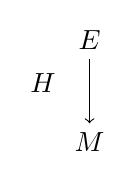
\begin{tikzpicture}[x=1cm,y=1cm,every node/.style={inner sep=1pt}]
\node at (0,.65) {$E$};
\node at (0,-.65) {$M$};
\node at (-.59,.10) {$H$};
\draw[->] (0,.41) -- (0,-.41);
\end{tikzpicture}}\endgroup}
\end{GelfandAdjacentEvidence}
\begin{GelfandAdjacentEvidence}{GELFAND-P000551}{3}

principal bundle and its automorphism group

It projects onto \(G_1\) with fiber \(G_2\)
\Incomplete{GELFAND-P000551}{bundle-old}{The rectangular entry below the diagram is densely crossed out and illegible.}
\end{GelfandAdjacentEvidence}
\begin{GelfandAdjacentEvidence}{GELFAND-P000551}{4}

\[
e^H=H_0\oplus H\oplus S^2(H)\oplus S^3(H)\oplus\ldots
\]
\Unclear{GELFAND-P000551}{fock-upper-marks}{Two horizontal strokes and a small loop between them stand above \(H,\oplus,S^2(H)\). Their meaning and attachment remain unresolved.}
\end{GelfandAdjacentEvidence}
\begin{GelfandAdjacentEvidence}{GELFAND-P000551}{5}

(\(H_0\) is one-dimensional; \(S^k(H)\) is a symm. power
\[
1\qquad \xi\qquad\frac{\xi\otimes\xi}{2!}
\qquad\qquad
|\xi|^2=\sum\frac{|\xi_n|^2}{n!}
\]
\Unclear{GELFAND-P000551}{fock-product}{The circled sign in the numerator provisionally reads \(\otimes\).}
\end{GelfandAdjacentEvidence}
\begin{GelfandAdjacentEvidence}{GELFAND-P000551}{6}


\uline{Gurevich.}\quad \uwave{On the K.–d.–V. eq. by Whitham’s method}.
\Unclear{GELFAND-P000551}{gurevich-old}{The ending of the abbreviated word for “equation” is overwritten in the Russian. Its exact reading remains unresolved.}
\end{GelfandAdjacentEvidence}



\Needspace{7\baselineskip}
\begin{GelfandAdjacentEvidence}{GELFAND-P000552}{1}
\SourcePage{GELFAND-P000552}{unlabelled}
\uline{1/\mbox{$\overline{\underline{IV}}$}-74.}\qquad
\uwave{Gelfand’s sem..}

\uwave{Yura Koblents.}\qquad\uwave{On the asymptotics of the eigenvalues of the Laplace oper..}

\hspace{2em}(from Leningrad)\par
\(M\) — closed Riem. manif., \(\Delta\) — Beltrami–Laplace oper..
\[
\lambda_0=0,\qquad 0\le\lambda_1\le\lambda_2\le\ldots
\qquad\text{— spectrum.}
\]
\[
Z(s)=\operatorname{Tr}\exp(-s\Delta)=\sum_i e^{-\lambda_i s}
\]
\[
\Delta f=\frac{1}{\sqrt g}\frac{\partial}{\partial x^i}
\left(\sqrt g\, g^{ij}\frac{\partial f}{\partial x^j}\right),
\qquad\text{where }\underline{g=\det\Vert g_{ij}\Vert},
\]
\Incomplete{GELFAND-P000552}{laplacian-old}{There is a densely crossed-out entry between the equals sign and \(1/\sqrt g\). A stroke on the right cannot confidently be separated from the cancellation.}
\end{GelfandAdjacentEvidence}
\begin{GelfandAdjacentEvidence}{GELFAND-P000552}{2}

\[
\uwave{\mbox{$\displaystyle E(m,m',t)=\sum e^{-\lambda_i t}\varphi_i(m)\varphi_i(m').$}}
\]
\Unclear{GELFAND-P000552}{kernel-functions}{The letter in both factors provisionally reads \(\varphi\).}
\end{GelfandAdjacentEvidence}
\begin{GelfandAdjacentEvidence}{GELFAND-P000552}{3}

\[
Z(s)=\int E(m,m,s)\,dm
\]

\uline{Minakshisundaram}, \uline{1949}
\[
Z(t)=(4\pi t)^{-n/2}(a_0+a_1t+a_2t^2+\ldots),
\qquad t\to0.
\]
\[
n=\dim M,\qquad a_0=\operatorname{vol} M,\qquad \operatorname{Re}t>0.
\]
\[
a_1=\int_M \frac{\tau}{6}\,dV,
\qquad\text{where }\tau\text{ — scal. curvature}
\]
\[
\tau=\sum_{\alpha\beta[?]\beta}R_{\alpha\beta[\ldots]}^{\alpha\beta}
\]
\Unclear{GELFAND-P000552}{scalar-indices}{The sum index shows an initial \(\alpha\beta\) and a final \(\beta\), with overwritten strokes between them. Two signs after the lower \(\alpha\beta\) of \(R\) are crossed out.}
\end{GelfandAdjacentEvidence}
\begin{GelfandAdjacentEvidence}{GELFAND-P000552}{4}

\[
a_2=\frac1{360}\int\left(2|R|^2-2|\rho|^2+5\tau^2\right)
\]
\(R\) — curvature tensor; \(\rho\) — Ricci tensor,
\[
\rho_{ij}=\sum_\alpha R_{i\alpha j}^{\alpha}
\]
\Unclear{GELFAND-P000552}{ricci-indices}{There is a heavily overwritten mark after the lower \(j\) of \(R\). The original stroke is illegible.}
\end{GelfandAdjacentEvidence}
\begin{GelfandAdjacentEvidence}{GELFAND-P000552}{5}

\[
|R|^2=\sum R_{\alpha\beta\gamma\delta}^2
\qquad\text{in norm. coord.}\qquad
|R|^2=R_{\alpha\beta\gamma\delta}R^{\alpha\beta\gamma\delta}
\]
\[
|\rho|^2=\rho_{\alpha\beta}\rho^{\alpha\beta}
\]
\[
E(t,m,m')=(4\pi t)^{-n/2}
\left(u_0(m,m')+u_1(m,m')t+u_2(m,m')t^2+\ldots\right)
\]
\uwave{in a neighb. of the diagonal}.

\uwave{\mbox{$a_3$} — Sakai and the speaker} (independently).

\uline{G.}\quad\uline{Number of int. points in a disk}:
\[
a(r)=\pi r^2+\sum_{\lambda_n}\tau^{1/2}\sin\frac{\tau}{\lambda_n}
\]
\Unclear{GELFAND-P000552}{circle-formula}{The letter at the start of the formula provisionally reads \(r\). Both occurrences in the summand have a broad wavy top, provisionally read as \(\tau\).}
\end{GelfandAdjacentEvidence}
\begin{GelfandAdjacentEvidence}{GELFAND-P000552}{6}

(\(\lambda_n\) — zeros of the Riemann \(\zeta\)-func.) \quad\uwave{mod the Riemann hypothesis}

\uline{Schnirelmann.}\par
In the ball \(\lambda_n\) — lengths of closed billiard paths.
\SourceFigure{GELFAND-P000552}{billiard-word}{The first letter of “шаре” has three strokes.}
\end{GelfandAdjacentEvidence}

\[
\sum\delta(\lambda-\lambda_k)*\frac{\varepsilon}{\lambda^2+\varepsilon^2}=f(\lambda)
\]


\Needspace{7\baselineskip}
\begin{GelfandAdjacentEvidence}{GELFAND-P000553}{1}
\SourcePage{GELFAND-P000553}{83}
\[
f(\lambda)=f_0(\lambda)+\sum_k c_k\lambda^{\alpha_k}
\sin(\ell_k\lambda+\omega_k)
\]
There is exper. confirmation (Balian and Bloch)
\Unclear{GELFAND-P000553}{balian-name}{The end of the surname Balian is retraced. The reading of the final n is provisional.}
\end{GelfandAdjacentEvidence}
\begin{GelfandAdjacentEvidence}{GELFAND-P000553}{2}

(and even a precise statement).
\[
\sum e^{i\lambda_k z}=\operatorname{Sp}(e^{-z\Delta}).
\]
\SourceFigure{GELFAND-P000553}{trace-exponent}{The exponent on the left is \(i\lambda_k z\), and the one on the right is \(-z\Delta\).}
\end{GelfandAdjacentEvidence}
\begin{GelfandAdjacentEvidence}{GELFAND-P000553}{3}

\dashuline{contin. downward} (from the upper half-plane)

\dashuline{Twin probl.}:
\[
\lambda_{k+1}-\lambda_k>c\lambda_k^{-\nu}
\qquad\text{for general operators}
\]
\Unclear{GELFAND-P000553}{gap-exponent}{The letter after the minus has two converging strokes and provisionally reads \(\nu\).}
\end{GelfandAdjacentEvidence}
\begin{GelfandAdjacentEvidence}{GELFAND-P000553}{4}

\uwave{but on the circle they are double.} (stably asympt. double spectrum).

\(T^2\)\qquad \(g_{ij}\sim\delta_{ij}\)\qquad the theorem holds

\uline{Theorem}.
\[
\uwave{\mbox{$\displaystyle\min(\lambda_{k+1}-\lambda_k,\lambda_k-\lambda_{k-1})
< C_N\cdot k^{-N}$}},\qquad \forall N
\]
(Lazutkin, Schnirelmann)
\Unclear{GELFAND-P000553}{attribution}{The strokes leading into the last letters of “Schnirelmann” are overwritten. The underlying strokes are illegible.}
\end{GelfandAdjacentEvidence}
\begin{GelfandAdjacentEvidence}{GELFAND-P000553}{5}

(a small but finite perturbation) — stab.

For \(T^3\) this is \uline{no longer so}. (\uline{apparently}).
\[
\frac{\partial u}{\partial t}=i\sqrt{-\Delta}\,u;\qquad
\left.u\right|_{t=0}=\delta_x
\]
\Unclear{GELFAND-P000553}{wave-numerator}{The overwritten letter after \(\partial\) provisionally reads \(u\).}
\end{GelfandAdjacentEvidence}
\begin{GelfandAdjacentEvidence}{GELFAND-P000553}{6}

Its soln. \qquad \(u(x,y,t)\)
\[
\sum e^{i\lambda_k t}=\int_M u(x,x,t)\,dx=f(t);
\]
\Unclear{GELFAND-P000553}{trace-time}{The sign in the exponent of the sum and the final argument of the integrand are retraced. Both provisionally read \(t\).}
\end{GelfandAdjacentEvidence}
\begin{GelfandAdjacentEvidence}{GELFAND-P000553}{7}

singul. of \(u(x,y,t)\) where \(\lvert x-y\rvert=t\)

\SourceFigure{GELFAND-P000553}{loop}{%
\par\smallskip
\begingroup\color{black}\GelfandFitDiagram{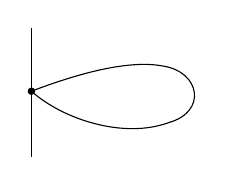
\begin{tikzpicture}[x=1cm,y=1cm]
\draw (0,-.83) -- (0,.80);
\draw (0,0) .. controls (.50,.19) and (1.20,.41) .. (1.67,.32)
  .. controls (2.14,.25) and (2.24,-.26) .. (1.74,-.40)
  .. controls (1.16,-.61) and (.39,-.35) .. (0,0) -- cycle;
\fill (0,0) circle (1.35pt);
\end{tikzpicture}}\endgroup}
\end{GelfandAdjacentEvidence}
\begin{GelfandAdjacentEvidence}{GELFAND-P000553}{8}

for some \(t\) bifurcations occ.
\Unclear{GELFAND-P000553}{bifurcation-ending}{The Russian ending of “bifurcations” is overwritten. The reading is provisional.}
\end{GelfandAdjacentEvidence}

singul. move at speed 1



\clearpage\section*{Chapter 8}

\Needspace{7\baselineskip}
\begin{GelfandAdjacentEvidence}{GELFAND-P000554}{1}
\SourcePage{GELFAND-P000554}{unlabelled}
\uline{2/\mbox{$\overline{\underline{IX}}$}-74.}\qquad
\uuline{Gelfand’s sem.}\quad (32nd year of the seminar)

\uline{Giusti}.

1. \uwave{Singularities} [crossed out] \uwave{and regularity}
\Unclear{GELFAND-P000554}{title-old}{Crossed-out strokes lie between “Singularities” and “and”. The original entry is illegible.}
\end{GelfandAdjacentEvidence}
\begin{GelfandAdjacentEvidence}{GELFAND-P000554}{2}

[crossed out] of solutions of non-linear elliptic (and parabolic) systems.
\Unclear{GELFAND-P000554}{line-prefix-old}{A separate crossed-out entry precedes “of solutions”. Its reading remains unresolved.}
\end{GelfandAdjacentEvidence}
\begin{GelfandAdjacentEvidence}{GELFAND-P000554}{3}

\uwave{Nash, De giorgi, Moser}. — Regularity: 1 equation linear
\sout{di\ldots} with discont. coeff. (Höld. coeff.)
\(\Rightarrow\) regul. for non linear with smooth coeff.
\Unclear{GELFAND-P000554}{linear-old}{There are crossed-out letters before “with”. The opening provisionally reads “di”.}
\end{GelfandAdjacentEvidence}
\begin{GelfandAdjacentEvidence}{GELFAND-P000554}{4}

\uline{Systems} — [crossed out] \uwave{false}. There are [?] coeff. and [?] solutions
\Unclear{GELFAND-P000554}{systems-old}{A heavily crossed-out sign follows the dash before “false”.}
\end{GelfandAdjacentEvidence}
\begin{GelfandAdjacentEvidence}{GELFAND-P000554}{5}

\Unclear{GELFAND-P000554}{systems-caption}{The Russian abbreviations before “coefficients” and “solutions” provisionally read “Быв. ср.” and “несгр.”.}
\end{GelfandAdjacentEvidence}
\begin{GelfandAdjacentEvidence}{GELFAND-P000554}{6}

1968 Miranda, Giusti — syst. with analytic coeff. with discont. solutions
\Unclear{GELFAND-P000554}{giusti-name}{The beginning of the surname Giusti is overwritten and the underlying strokes are illegible.}
\end{GelfandAdjacentEvidence}
\begin{GelfandAdjacentEvidence}{GELFAND-P000554}{7}

\hfill\rule{1.4cm}{.35pt}\enspace\(\cdot\)\enspace\rule{1.4cm}{.35pt}\par
\(\Sigma\) — singular set.
\begin{align*}
&(1)\quad \Sigma\text{ closed}\\
&(2)\quad \dim\Sigma<n-2
\end{align*}
\hfill\rule{1.4cm}{.35pt}\enspace\(\cdot\)\enspace\rule{1.4cm}{.35pt}\par

2. \uwave{Boundary value problems. for surfaces of prescribed mean curvature}.
\[
u:\Omega\longrightarrow\mathbb R \qquad \operatorname{graph}u=S
\]
\SourceFigure{GELFAND-P000554}{domain-outline}{%
\par\smallskip
\begingroup\color{black}\GelfandFitDiagram{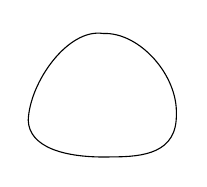
\begin{tikzpicture}[x=.95cm,y=.95cm]
\draw (.04,.52) .. controls (.06,1.03) and (.57,1.75) .. (1.04,1.68)
  .. controls (1.53,1.70) and (2.04,1.12) .. (2.02,.60)
  .. controls (2.03,.08) and (1.58,.03) .. (1.16,.03)
  .. controls (.50,.01) and (.05,.17) .. (.04,.52) -- cycle;
\end{tikzpicture}}\endgroup}
\end{GelfandAdjacentEvidence}
\begin{GelfandAdjacentEvidence}{GELFAND-P000554}{8}

\SourceFigure{GELFAND-P000554}{graph-sketch}{%
\par\smallskip
\begingroup\color{black}\GelfandFitDiagram{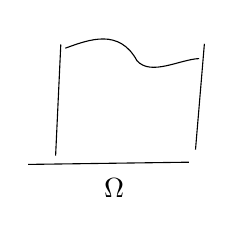
\begin{tikzpicture}[x=.94cm,y=.94cm,every node/.style={inner sep=1pt}]
\draw (0,0) -- (2.17,.03);
\draw (.37,.12) -- (.44,1.62);
\draw (2.26,.20) -- (2.38,1.63);
\draw (.50,1.57) .. controls (.83,1.69) and (1.23,1.84) .. (1.47,1.40)
  .. controls (1.66,1.19) and (2.05,1.42) .. (2.31,1.43);
\node[below] at (1.16,-.15) {$\Omega$};
\end{tikzpicture}}\endgroup}
\end{GelfandAdjacentEvidence}
\begin{GelfandAdjacentEvidence}{GELFAND-P000554}{9}

\[
H(x)=\frac{1}{n}\sum\frac{\partial}{\partial x_i}
\left(\frac{\partial u/\partial x_i}{\sqrt{1+|\operatorname{grad}u|^2}}\right)
\]
\(H\) is not very large (otherwise unsolvable). Depends on the geometry of the domain, the func. \(H(x)\) and so on

That is what will come next time.

\uuline{S. P. Novikov.} (and Dubrovin).

Abelian var. \(\xi_1,\ldots,\xi_{2n}\) — basis in \(\mathbb C^n\) (over \(\mathbb R\)),
\(T^{2n}\) — corresp. torus. Let the Abelian var. (algebraic var.).

How to describe all tori?

\uuline{\mbox{$n=2$}}\qquad \uwave{already nontrivial}.
\[
y^2=P_{2n+1}(x)\qquad\text{Riem. surface}\quad\Rightarrow\quad\text{torus.}
\]
\Incomplete{GELFAND-P000554}{cohomology-old}{A crossed-out entry before \(H^1\) provisionally begins “Вид…”. The rest is illegible.}
\end{GelfandAdjacentEvidence}
\begin{GelfandAdjacentEvidence}{GELFAND-P000554}{10}

\[
\underbrace{H^1(R,\mathbb C)/H^1(R,\mathbb Z)}_{\text{the torus is like this}}
\qquad \uwave{\mbox{$R\longrightarrow J^{2n}(R).$}}\quad(\text{torus})
\]
\[
k=0,\ldots,n-1,\qquad
\boxed{\omega_k=\frac{x^k\,dx}{\sqrt{P_{2n+1}(x)}}}
\quad\longleftarrow\quad\text{everywhere regular differentials}.
\]
Basis — the forms \(\omega_k\).
\[
P_{2n+1}(x)=\prod(x-x_\alpha).
\]
Everything is det. by the set of roots.

\SourceFigure{GELFAND-P000554}{moduli-maps}{%
\par\smallskip
\begingroup\color{black}\GelfandFitDiagram{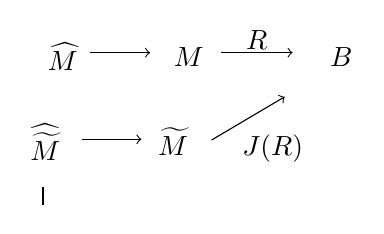
\begin{tikzpicture}[x=1cm,y=1cm,every node/.style={inner sep=1pt}]
\node (cover) at (0,0) {$\widehat M$};
\node (surfaces) at (1.60,0) {$M$};
\node (base) at (3.54,0) {$B$};
\draw[->] (.35,.05) -- (1.11,.05);
\draw[->] (2.01,.05) -- node[above] {$R$} (2.92,.05);
\node at (-.22,-1.09) {$\widehat{\widetilde M}$};
\node at (1.40,-1.08) {$\widetilde M$};
\draw[->] (.25,-1.05) -- (1.00,-1.05);
\draw[->] (1.89,-1.06) -- (2.82,-.51);
\node[right] at (2.24,-1.17) {$J(R)$};
\draw (-.25,-1.65) -- (-.25,-1.89);
\end{tikzpicture}}\endgroup\par\smallskip
The lower diagonal arrow ends below and to the left of the upper B. Its exact connection remains unresolved.}
\end{GelfandAdjacentEvidence}


\(M\) — collection of Riem. surfaces

\(B\) — Siegel upper half-space

(cover of the moduli set).

from the set of roots one constructs the polynomial, and from it the torus.


\Needspace{7\baselineskip}
\begin{GelfandAdjacentEvidence}{GELFAND-P000555}{1}
\SourcePage{GELFAND-P000555}{unlabelled}
\begin{gather*}
p_1,p_2,q_1,q_2,c,d.\qquad \mathbb C^6\text{ or }\mathbb C^4_{c,d}\\
J_1=p_1p_2+V(q_1,q_2)\\
J_2=p_1^2-2q_1p_1p_2+2(q_2-c)p_2^2+\mathcal D(q_1,q_2)\\
\Omega=\sum_{\alpha=1}^{2}dp_\alpha\wedge dq_\alpha.
\end{gather*}
\(\langle J_1,J_2\rangle\equiv0.\) \quad Poisson br.
\[
V=-\left(\frac{q_2^2}{2}+\frac52q_1^2q_2+\frac52q_1^4\right)+c_1q_1^2-d_1q_1
\]
\Unclear{GELFAND-P000555}{potential-symbol}{The sign before the equals sign is overwritten. It has two upper strokes and provisionally reads \(V\).}
\end{GelfandAdjacentEvidence}
\begin{GelfandAdjacentEvidence}{GELFAND-P000555}{2}

\[
\mathcal D=q_1^5+2c_1q_1^3+d_1q_1^2-4q_1q_2^2+4c_1q_1q_2-2d_1q_2
\]
\[
[X_{J_1},X_{J_2}]=0.\quad\text{Obtain 2 commut. fields.}
\]
The corresp. orbits — an Abelian var.
\[
\left.\underline{\begin{aligned}
J_1&=\mathrm{const}\\
J_2&=\mathrm{const}
\end{aligned}}\right\}\quad\text{\uuline{torus.}}
\]
\Unclear{GELFAND-P000555}{orbit-old}{A crossed-out entry left of the equations starts with a \(J\)-like form. The rest is illegible.}
\end{GelfandAdjacentEvidence}
\begin{GelfandAdjacentEvidence}{GELFAND-P000555}{3}

\uwave{Corollary}: the coll. of them all — a unirat. variety.
\[
R:\quad y^2=x^5+\frac{c_1}{4}x^3-\frac{d_1}{16}x^2+
\left(\frac{J_1}{32}+\frac{c_1^2}{4}\right)x+\frac{J_2}{2^8}+\frac{c_1d_1}{2^7}
\]
\hfill\rule{1.4cm}{.35pt}\enspace\(\cdot\)\enspace\rule{1.4cm}{.35pt}\par
\(R\) — Riem. surface, \quad \(S^nR\) — symm. power of \(R\).

\((J_1,\ldots,J_n)\) and symmetrization.
\Unclear{GELFAND-P000555}{symmetric-label}{Both letters in the row before “and symmetrization” have a hook. The reading \(J\) is provisional.}
\end{GelfandAdjacentEvidence}
\begin{GelfandAdjacentEvidence}{GELFAND-P000555}{4}

\begin{gather*}
S^nR\longrightarrow J(R).\\
(P_1,\ldots,P_n)\xrightarrow{A}(\alpha_1,\ldots,\alpha_n)
\qquad\text{Abel map.}
\end{gather*}
(\uline{Abel’s theor.} — it is an isomorphism).
\SourceFigure{GELFAND-P000555}{abel-paths}{%
\par\smallskip
\begingroup\color{black}\GelfandFitDiagram{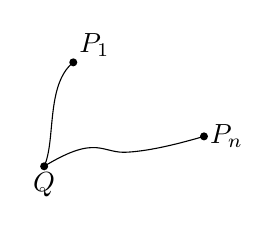
\begin{tikzpicture}[x=1cm,y=1cm,every node/.style={inner sep=2pt}]
\draw (0,0) .. controls (.15,.32) and (.02,1.04) .. (.37,1.32);
\draw (0,0) .. controls (.69,.42) and (.73,.15) .. (1.07,.18)
  .. controls (1.37,.20) and (1.72,.29) .. (2.03,.38);
\fill (0,0) circle (1.45pt) node[below] {$Q$};
\fill (.37,1.32) circle (1.45pt) node[above right] {$P_1$};
\fill (2.03,.38) circle (1.45pt) node[right] {$P_n$};
\end{tikzpicture}}\endgroup\par\smallskip
The upper curve thickens at \(P_1\). An arrowhead cannot be distinguished.}
\end{GelfandAdjacentEvidence}
\begin{GelfandAdjacentEvidence}{GELFAND-P000555}{5}

\[
(P_1,\ldots,P_n)\longrightarrow
\left(\underbrace{\sum_{k=1}^{n}\oint_Q^{P_k}\omega_s}
_{\substack{\vert\vert\\ \alpha_s}}\right)
\]
\SourceFigure{GELFAND-P000555}{abel-integral}{A loop is visible on the integral sign. Two short strokes stand above \(\alpha_s\) below the bracket.}
\end{GelfandAdjacentEvidence}
\begin{GelfandAdjacentEvidence}{GELFAND-P000555}{6}

\[
L=-\frac{d^2}{dx^2}+u(x),
\]
\uwave{\mbox{$u(x+T)=u(x)$}}\quad or\quad \uwave{quasiperiodic}.
\[
\text{Eigenfunc.}\qquad
\uwave{\mbox{$L\Psi(x,E)=E\Psi,$}}
\]
\[
\Psi(x+T)=\lambda\Psi(x),\qquad |\lambda|=1,\qquad\lambda=e^{ip(E)}
\]
(Bloch eigenfuncs.)

For almost periodic [crossed out] the collection of such eigenfuncs. does not form a complete system.
\Incomplete{GELFAND-P000555}{almost-periodic-old}{A short densely crossed-out entry follows the Russian abbreviation for “periodic”.}
\end{GelfandAdjacentEvidence}

\[
\left.\Psi\right|_{x_0}=1 \quad\text{— normalization}
\]
\[
\Psi(x,E,x_0)\qquad (\Psi,\overline\Psi)\quad\text{— 2 eigenfuncs.}
\]
branches in \(E\) at the endpoints of the spectral intervals. Obtain a Riem. surface of inf. genus. 2 sheets, since there are 2 eigenfuncs.


\Needspace{7\baselineskip}
\begin{GelfandAdjacentEvidence}{GELFAND-P000556}{1}
\SourcePage{GELFAND-P000556}{unlabelled}
The set of pot. with given band structure — the Jacobian var. of this Riem. surface (there are formulas)
\Unclear{GELFAND-P000556}{zonal-overwrite}{The first strokes in the Russian word for “band” are overwritten.}
\end{GelfandAdjacentEvidence}
\begin{GelfandAdjacentEvidence}{GELFAND-P000556}{2}

\SourceFigure{GELFAND-P000556}{spectrum-line}{%
\par\smallskip
\begingroup\color{black}\GelfandFitDiagram{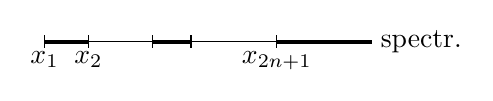
\begin{tikzpicture}[x=.62cm,y=.66cm,every node/.style={inner sep=1pt}]
\draw (0,0) -- (6.7,0);
\draw[line width=1.5pt] (0,0) -- (.90,0);
\draw[line width=1.5pt] (2.22,0) -- (3.00,0);
\draw[line width=1.5pt] (4.76,0) -- (6.70,0);
\foreach \position in {0,.90,2.22,3.00,4.76}
  \draw (\position,-.12) -- (\position,.12);
\node[below] at (0,-.12) {$x_1$};
\node[below] at (.90,-.12) {$x_2$};
\node[below] at (4.76,-.12) {$x_{2n+1}$};
\node[right] at (6.82,0) {\uuline{spectr.}};
\end{tikzpicture}}\endgroup}
\end{GelfandAdjacentEvidence}
\begin{GelfandAdjacentEvidence}{GELFAND-P000556}{3}

Pot. with given band structure — the corresp. torus (Jacobian var.).
\hfill\(\cdots\cdots\cdots\cdots\cdots\cdots\cdots\cdots\)\par

\uline{9/\mbox{$\overline{\underline{IX}}$}-74}\enspace.\qquad\uline{Gelfand’s sem..}

\uline{Bessaga} (\uwave{Warsaw}).\quad \uwave{Anderson’s \mbox{$Z$}-sets and their applications}.
\hfill (R. D. Anderson)\par
\(X\) — a complete metriz. space. \quad \(A\subset X,\ \overline{A}=A\).

\(A\) is called a \(Z\)-set if \(\forall\) cont. maps
\[
f:\underbrace{I^\infty}_{\text{Hilb. cube}}\longrightarrow X,\qquad
\forall\varepsilon>0,\qquad
\exists g:I^\infty\longrightarrow X\setminus A,\qquad
\rho(f,g)<\varepsilon.
\]
\[
\underline{Q=[-1,1]^\infty,\qquad P=(-1,1)^\infty.}
\qquad(Q\setminus P)\text{ — \(Z\)-set}
\]
\uline{Prop.}: \(1^\circ\). If \(A,B\) are \(Z\)-sets (in \(Q\)),
then \(f:A\xrightarrow{\sim} B\) extends to a \sout{homeo} homeom. of the entire space.
\Unclear{GELFAND-P000556}{property-number}{The numeral of \(1^\circ\) is heavily overwritten. The small circle and period are distinguishable.}
\end{GelfandAdjacentEvidence}
\begin{GelfandAdjacentEvidence}{GELFAND-P000556}{4}

\Unclear{GELFAND-P000556}{extension-old}{The crossed-out abbreviation before “homeom.” provisionally reads “homeo”.}
\end{GelfandAdjacentEvidence}
\begin{GelfandAdjacentEvidence}{GELFAND-P000556}{5}


\uwave{\mbox{$Z_\sigma$}-set} — a countable union of \(Z\)-sets.

\(2^\circ\). There exists a maximal \(Z_\sigma\)-set
\hfill\rule{1.4cm}{.35pt}\enspace\(\cdot\)\enspace\rule{1.4cm}{.35pt}\par

\uline{Gelfand}

Consid. \(\mathbb R^\infty\) in the Tych. topology and the space \(S\) of rays [crossed out] issuing from 0 in the nat. topology.
Prove that on \(S\) every cont. func. is [crossed out] \uline{const}
\Incomplete{GELFAND-P000556}{rays-old}{There is a densely crossed-out entry between “rays” and “issuing”.}
\end{GelfandAdjacentEvidence}
\begin{GelfandAdjacentEvidence}{GELFAND-P000556}{6}

\Unclear{GELFAND-P000556}{constant-old}{A small crossed-out mark precedes “const”. Its reading remains unresolved.}
\end{GelfandAdjacentEvidence}
\begin{GelfandAdjacentEvidence}{GELFAND-P000556}{7}

(Gelf., Fuks. Funct. Anal. I, 4).
\hfill\rule{1.4cm}{.35pt}\enspace\(\cdot\)\enspace\rule{1.4cm}{.35pt}\par
\uline{Bessaga}. All separab. Fréchet spaces are homeomorphic.

\uuline{Giusti.}\qquad \(\Omega\subset\mathbb R^n\)
\SourceFigure{GELFAND-P000556}{hatched-domain}{%
\par\smallskip
\begingroup\color{black}\GelfandFitDiagram{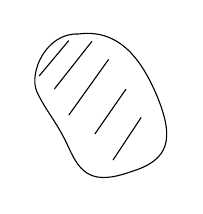
\begin{tikzpicture}[x=.92cm,y=.92cm]
\draw (.13,1.20) .. controls (.01,1.48) and (.27,2.02) .. (.70,2.00)
  .. controls (1.29,2.08) and (1.59,1.61) .. (1.79,1.14)
  .. controls (2.03,.55) and (1.96,.26) .. (1.43,.10)
  .. controls (.90,-.09) and (.73,.07) .. (.57,.43)
  .. controls (.40,.80) and (.27,.91) .. (.13,1.20) -- cycle;
\draw (.16,1.42) -- (.57,1.91) (.37,1.24) -- (.89,1.90)
      (.57,.88) -- (1.12,1.65) (.93,.62) -- (1.36,1.24)
      (1.18,.26) -- (1.57,.85);
\end{tikzpicture}}\endgroup}
\end{GelfandAdjacentEvidence}
\begin{GelfandAdjacentEvidence}{GELFAND-P000556}{8}

\[
\left\{\begin{aligned}
\sum_{i=1}^{n}D_i\left\{\frac{D_i u}{\sqrt{1+|Du|^2}}\right\}
&=-H(x,u)\quad\text{in }\Omega,\\
u&=\phi\quad\text{on }\partial\Omega
\end{aligned}\right.
\qquad D_i=\frac{\partial}{\partial x_i}.
\]
\(n\) times the mean curvature \(=\) the left-hand side of the eq.

\(\underline{H\equiv0}\quad\Rightarrow\quad\text{minimal surface.}\)
\SourceFigure{GELFAND-P000556}{graph-cylinder}{%
\par\smallskip
\begingroup\color{black}\GelfandFitDiagram{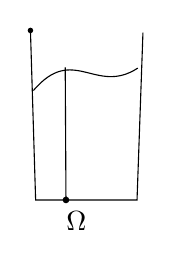
\begin{tikzpicture}[x=.94cm,y=.92cm,every node/.style={inner sep=1pt}]
\draw (0,2.34) -- (.07,0) -- (1.44,0) -- (1.52,2.31);
\draw (.04,1.51) .. controls (.58,2.16) and (.88,1.44) .. (1.45,1.82);
\draw (.47,1.83) -- (.48,0);
\fill (.48,0) circle (1.2pt);
\fill (0,2.34) circle (1pt);
\node[below] at (.62,-.12) {$\Omega$};
\end{tikzpicture}}\endgroup\par\smallskip
A dark mark sits at the lower end of the inner vertical stroke. Its shape is indistinct.}
\end{GelfandAdjacentEvidence}
\begin{GelfandAdjacentEvidence}{GELFAND-P000556}{9}

\uline{Example 1}.\quad \(\Omega,\quad n=2,\quad H=0\)
\SourceFigure{GELFAND-P000556}{annulus}{%
\par\smallskip
\begingroup\color{black}\GelfandFitDiagram{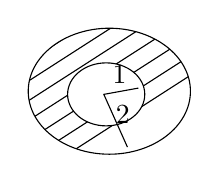
\begin{tikzpicture}[x=1cm,y=1cm,every node/.style={inner sep=1pt}]
\begin{scope}
\pgfseteorule
\clip (0,0) ellipse (1.03 and .80) (-.04,-.04) ellipse (.49 and .40);
\foreach \height in {-1.2,-.95,-.70,-.45,-.20,.05,.30,.55,.80}
  \draw (-1.15,\height) -- (1.12,{\height+1.46});
\end{scope}
\draw (0,0) ellipse (1.03 and .80) (-.04,-.04) ellipse (.49 and .40);
\draw (.37,.04) -- (-.07,-.04) -- (.23,-.71);
\node at (.13,.21) {$1$};
\node at (.17,-.30) {$2$};
\end{tikzpicture}}\endgroup\par\smallskip
circular annulus. The labels 1 and 2 stand beside the two radial strokes.}
\end{GelfandAdjacentEvidence}
\begin{GelfandAdjacentEvidence}{GELFAND-P000556}{10}

\[
\phi=\begin{cases}
0&|x|=2\\
M&|x|=1
\end{cases}
\]
\uwave{Solution}:\quad \(u(r),\qquad \uwave{\mbox{$r=|x|$}}.\)
\begin{gather*}
u(r)=c\log\frac{2+\sqrt{4-c^2}}{r+\sqrt{r^2-c^2}},\qquad 0\le c\le1,\\
u(1)=M\quad\Rightarrow\quad u(1)\le\log(2+\sqrt3)=M_0.
\end{gather*}
\Unclear{GELFAND-P000556}{radial-overwrites}{The opening strokes of \(u(r)\) and \(u(1)\) are heavily overwritten. The underlying forms are illegible.}
\end{GelfandAdjacentEvidence}



\Needspace{7\baselineskip}
\begin{GelfandAdjacentEvidence}{GELFAND-P000557}{1}
\SourcePage{GELFAND-P000557}{unlabelled}
For \(M>M_0\) there are no solutions.

\uline{Exper. check}: soap bubble\par
we carefully lift the \uline{stick}
\hfill\uwave{steak.}\par
\SourceFigure{GELFAND-P000557}{english-word}{Below the Russian word for “stick” the manuscript reads “steak.” with a wavy underline.}
\end{GelfandAdjacentEvidence}
\begin{GelfandAdjacentEvidence}{GELFAND-P000557}{2}

\SourceFigure{GELFAND-P000557}{soap-surfaces}{%
\par\smallskip
\begingroup\color{black}\GelfandFitDiagram{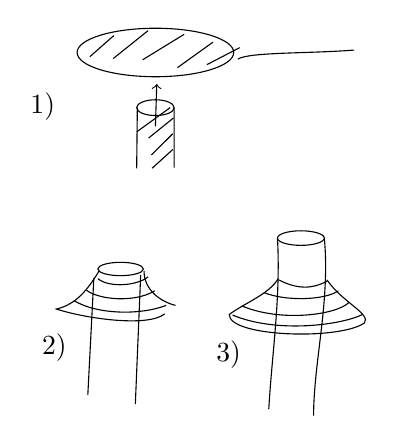
\begin{tikzpicture}[x=.85cm,y=.77cm,every node/.style={inner sep=1pt}]
\node[left] at (.30,1.05) {1)};
\draw (1.75,1.94) ellipse (1.17 and .40);
\draw (2.98,1.83) .. controls (3.15,1.95) and (4.05,1.92) .. (4.72,1.98);
\draw (.77,1.87) -- (1.13,2.22) (1.12,1.84) -- (1.64,2.30)
      (1.56,1.82) -- (2.18,2.24) (2.08,1.69) -- (2.61,2.11)
      (2.52,1.74) -- (3.01,2.02);
\draw (1.47,.03) -- (1.48,1.03) (2.03,.04) -- (2.03,1.03);
\draw (1.75,1.03) ellipse (.28 and .13);
\draw (1.47,.63) -- (1.97,1.03) (1.65,.53) -- (2.02,.86)
      (1.69,.25) -- (2.01,.60) (1.70,.03) -- (2.01,.34);
\draw[->] (1.75,.72) -- (1.77,1.42);
\begin{scope}[yshift=-3.05cm]
\node at (.24,1.03) {2)};
\draw (1.23,2.33) ellipse (.34 and .11);
\draw (.91,2.30) .. controls (.74,1.99) and (.56,1.74) .. (.27,1.67)
  .. controls (.68,1.52) and (1.63,1.36) .. (1.89,1.59);
\draw (1.58,2.30) .. controls (1.58,1.98) and (1.83,1.79) .. (2.05,1.73);
\draw (.89,2.17) .. controls (1.07,2.01) and (1.49,2.06) .. (1.64,2.20)
      (.72,1.98) .. controls (.91,1.82) and (1.44,1.77) .. (1.74,1.97)
      (.53,1.81) .. controls (.89,1.57) and (1.54,1.57) .. (1.91,1.73);
\draw (.83,2.18) -- (.74,.25) (1.53,2.23) -- (1.45,.10);
\begin{scope}[xshift=2.23cm]
\node at (.22,.92) {3)};
\draw (1.30,2.84) ellipse (.35 and .12);
\draw (.95,2.84) .. controls (1.00,1.87) and (.87,.95) .. (.82,.02);
\draw (1.65,2.84) .. controls (1.74,1.80) and (1.49,.80) .. (1.49,-.09);
\draw (.96,2.17) .. controls (.82,1.91) and (.46,1.77) .. (.23,1.58)
  .. controls (.22,1.21) and (1.87,1.15) .. (2.25,1.44)
  .. controls (2.35,1.59) and (1.92,1.78) .. (1.69,2.15);
\draw (.97,2.15) .. controls (1.25,1.99) and (1.48,2.00) .. (1.69,2.13)
      (.75,1.94) .. controls (1.09,1.79) and (1.67,1.82) .. (1.86,1.97)
      (.42,1.72) .. controls (1.00,1.45) and (1.83,1.57) .. (2.02,1.78)
      (.28,1.57) .. controls (.95,1.26) and (1.92,1.41) .. (2.22,1.58);
\end{scope}
\end{scope}
\end{tikzpicture}}\endgroup}
\end{GelfandAdjacentEvidence}
\begin{GelfandAdjacentEvidence}{GELFAND-P000557}{3}


if it is a wire ring, then
\SourceFigure{GELFAND-P000557}{wire-ring}{%
\par\smallskip
\begingroup\color{black}\GelfandFitDiagram{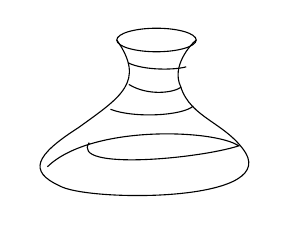
\begin{tikzpicture}[x=.9cm,y=.83cm]
\draw (0,1.89) ellipse (.56 and .18);
\draw (-.56,1.89) .. controls (-.15,1.25) and (-.50,1.02) .. (-1.10,.55)
  .. controls (-1.72,.12) and (-1.81,-.12) .. (-1.37,-.34)
  .. controls (-1.00,-.58) and (1.67,-.61) .. (1.26,.16)
  .. controls (.98,.63) and (.48,.69) .. (.34,1.18)
  .. controls (.21,1.48) and (.47,1.81) .. (.56,1.89);
\draw (-.40,1.54) .. controls (-.17,1.42) and (.27,1.43) .. (.42,1.48)
      (-.39,1.21) .. controls (-.12,1.03) and (.24,1.08) .. (.35,1.17)
      (-.65,.83) .. controls (-.32,.69) and (.37,.73) .. (.52,.88);
\draw (-1.54,-.05) .. controls (-.92,.60) and (.83,.52) .. (1.16,.27)
  .. controls (.59,.07) and (-1.22,-.11) .. (-.95,.32);
\end{tikzpicture}}\endgroup}
\end{GelfandAdjacentEvidence}
\begin{GelfandAdjacentEvidence}{GELFAND-P000557}{4}


\uline{Example 2}.\quad \(n=1,\quad \Omega=(-1,1)\)
\[
\uwave{\mbox{$u=3x^{1/3}$}}
\]
\Unclear{GELFAND-P000557}{cube-root-symbol}{The initial letter is overwritten. Its final outline provisionally reads \(u\).}
\end{GelfandAdjacentEvidence}
\begin{GelfandAdjacentEvidence}{GELFAND-P000557}{5}

\[
\left(\frac{u'}{\sqrt{1+u'^2}}\right)'=
\underbrace{-\frac23 x^{1/3}\left(1+x^{4/3}\right)^{-3/2}}_{\text{\uline{cont.}}}
\]
\SourceFigure{GELFAND-P000557}{derivative-power}{The exponent on the first \(x\) is \(1/3\). The exponent on the second \(x\) is \(4/3\).}
\end{GelfandAdjacentEvidence}
\begin{GelfandAdjacentEvidence}{GELFAND-P000557}{6}

[crossed out] \(u\) — nondiff.
\Unclear{GELFAND-P000557}{nondifferentiable-old}{The crossed-out Russian entry may begin “об…”. Its end is illegible.}
\end{GelfandAdjacentEvidence}
\begin{GelfandAdjacentEvidence}{GELFAND-P000557}{7}

\[
\uwave{\mbox{$u(-1)=-3,\qquad u(1)=3$}}
\]
Let
\[
u(-1)=3,\qquad u(1)=3+A
\]
\SourceFigure{GELFAND-P000557}{boundary-sign}{After “Let” the manuscript reads \(u(-1)=3\).}
\end{GelfandAdjacentEvidence}

\begin{gather*}
\frac{u'}{\sqrt{1+u'^2}}=(1+x^{4/3})^{-1/2}\\
u'\le x^{-2/3}\\
u(x)\le -3+\int_{-1}^{x}t^{-2/3}\,dt=3x^{1/3}
\end{gather*}
\hfill\rule{1.4cm}{.35pt}\enspace\(\cdot\)\enspace\rule{1.4cm}{.35pt}\par
\[
\mathcal F(u)=\int_\Omega\sqrt{1+|Du|^2}\,dx+\int_\Omega\lambda(x,u)\,dx
\]
\hfill Need to find \uuline{min}.\par
\[
\lambda(x,t)=\int_0^t H(x,s)\,ds
\]
Under the cond. \(|u'|\le K\) there is a \uwave{min}. (otherwise none).

\(u_k\) — soln. Let \(k\to+\infty\). \qquad \(u_k\to u_0\) ?
\hfill\rule{1.4cm}{.35pt}\enspace\(\cdot\)\enspace\rule{1.4cm}{.35pt}\par
\(u\) — Lip-contin. solut.\qquad \(A\subset\Omega\)
\begin{gather*}
\int_A H(x)\,dx=\int_{\partial A} n_i\frac{D_i u}{\sqrt{1+|Du|^2}}\,dH_{n-1}\\
\left|\int_A H(x)\,dx\right|\le(1-\varepsilon_0)H_{n-1}(\partial A)\\
\boxed{1-\varepsilon_0=\sup_{\Omega}\frac{|Du|}{\sqrt{1+|Du|^2}}.}
\end{gather*}
\uwave{Therefore \mbox{$H$} is not very large}.
\hfill\rule{1.4cm}{.35pt}\enspace\(\cdot\)\enspace\rule{1.4cm}{.35pt}\par


\Needspace{7\baselineskip}
\begin{GelfandAdjacentEvidence}{GELFAND-P000558}{1}
\SourcePage{GELFAND-P000558}{unlabelled}
\(\textcircled{1}\qquad H^{1,1}=W_1^1\qquad\parallel\)
\[
\mathcal F(u)=\int_\Omega\sqrt{1+|Du|^2}\,dx+
\int_\Omega\lambda(x,u)\,dx+
\int_{\partial\Omega}|u-\phi|\,dH_{n-1}
\]
\(BV(\Omega)\) \(=\) \(L^1\) funcs., whose first derivs. are measures (Radon).
\[
\begin{gathered}
\text{i.e.}\quad f\in BV \iff f\in L^1,\\
\sup\left\{\int_\Omega f\operatorname{div}\vec g\,dx,\quad
\vec g\in C_0^1(\Omega),\ |g|\le1\right\}<+\infty
\end{gathered}
\]
\[
\sup=\int_\Omega \overset{\vert\vert}{|Df|}\,dx
\]
\Unclear{GELFAND-P000558}{variation-bars}{Two separate strokes stand above \(Df\). The crossed-out mark to their left is illegible.}
\end{GelfandAdjacentEvidence}
\begin{GelfandAdjacentEvidence}{GELFAND-P000558}{2}

\uwave{Area}\quad \underline{\(f\in BV.\)}
\[
\begin{aligned}
\mathcal A(f)&=\int\sqrt{1+|Df|^2}\,dx\underset{\mathrm{def}}{=}\\
&\sup\left\{\int_\Omega(g_0+f\operatorname{div}\vec g)\,dx,\quad
g_0,g\in C_0^1,\quad g_0^2+|g|^2\le1\right\}.
\end{aligned}
\]
\Unclear{GELFAND-P000558}{area-test}{The left stroke at \(g\) merges with the letter. The reading \(|g|^2\) is provisional.}
\end{GelfandAdjacentEvidence}
\begin{GelfandAdjacentEvidence}{GELFAND-P000558}{3}

\uwave{area}.

\((\mathcal A f)\) lower semicont. with respect to \(L^1\) \sout{cont\ldots y}.
\Unclear{GELFAND-P000558}{semicontinuity-old}{The crossed-out English word provisionally reads “cont…y”. The full word remains unresolved.}
\end{GelfandAdjacentEvidence}
\begin{GelfandAdjacentEvidence}{GELFAND-P000558}{4}

\textcircled{2} Bounded sets in \(BV\) are relatively compact in \(L_1\)
\par\noindent\(\cdots\cdots\cdots\cdots\cdots\cdots\cdots\cdots\cdots\)

\uuline{Dubrovin}.
\[
L=-\frac{d^2}{dx^2}+u(x),\qquad
\uwave{\mbox{$u(x+T)=u(x)$}}
\]
\(E\) — spectral parameter.
\SourceFigure{GELFAND-P000558}{spectral-lines}{%
\par\smallskip
\begingroup\color{black}\GelfandFitDiagram{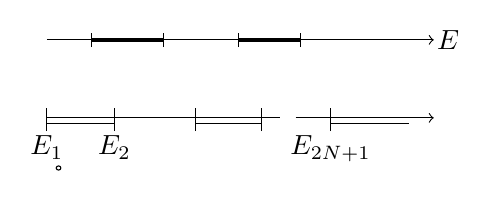
\begin{tikzpicture}[x=.78cm,y=.7cm,every node/.style={inner sep=1pt}]
\draw[->] (0,0) -- (6.30,0) node[right] {$E$};
\draw[line width=1.35pt] (.73,0) -- (1.90,0) (3.12,0) -- (4.13,0);
\foreach \x in {.73,1.90,3.12,4.13}
  \draw (\x,-.13) -- (\x,.13);
\begin{scope}[yshift=-.99cm]
\draw (0,0) -- (3.80,0);
\draw[->] (4.05,0) -- (6.30,0);
\draw (0,-.11) -- (1.10,-.11) (2.42,-.11) -- (3.49,-.11)
      (4.62,-.11) -- (5.90,-.11);
\foreach \x in {0,1.10,2.42,3.49,4.62}
  \draw (\x,-.24) -- (\x,.18);
\node[below] at (0,-.27) {$E_1$};
\draw (.19,-.91) circle (.038);
\node[below] at (1.10,-.27) {$E_2$};
\node[below] at (4.62,-.27) {$E_{2N+1}$};
\end{scope}
\end{tikzpicture}}\endgroup\par\smallskip
A small unfilled loop stands below \(E_1\). Its meaning remains unresolved.}
\end{GelfandAdjacentEvidence}
\begin{GelfandAdjacentEvidence}{GELFAND-P000558}{5}

Sometimes the gaps disappear.

Let \(u(x)\) — a finite-gap potential

Let \(R(E)=\prod(E-E_i)\)

Consid. the Riem. surface of the func. \(\sqrt{R(E)}\) — denote by \(\Gamma_N\).

\uwave{Bloch eigenfuncs. continue analyt. to \mbox{$\Gamma_N\setminus\infty$}} [crossed out]
\Incomplete{GELFAND-P000558}{continuation-old}{The parenthetical entry at the right is densely crossed out and illegible.}
\end{GelfandAdjacentEvidence}
\begin{GelfandAdjacentEvidence}{GELFAND-P000558}{6}

\hfill\underline{(meromorphically)}\par
\uwave{\mbox{$N$} — genus.}

and has \(N\) poles and \(N\) zeros

\uwave{Bloch eigenfunc.:} \(\Psi(x,E,x_0)\)

Poles \(\gamma_i(x_0)\).
\hfill \(\parallel\) there is a natural proj.\par
\[
\uwave{\mbox{$\Gamma_N\longrightarrow\mathbb C_E.$}}
\]
\hfill 2-sheeted covering\par
\SourceFigure{GELFAND-P000558}{covering-ovals}{%
\par\smallskip
\begingroup\color{black}\GelfandFitDiagram{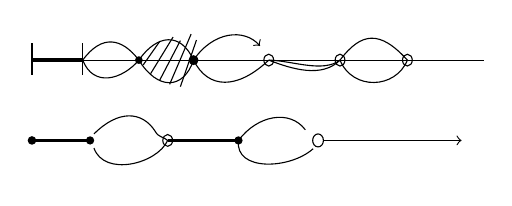
\begin{tikzpicture}[x=.62cm,y=.75cm]
\draw (0,0) -- (9.25,0);
\draw[line width=1.35pt] (0,0) -- (1.04,0);
\draw (0,-.25) -- (0,.29) (1.04,-.25) -- (1.04,.29);
\draw (1.04,0) .. controls (1.43,.44) and (1.84,.38) .. (2.19,0)
  .. controls (1.85,-.33) and (1.26,-.47) .. (1.04,0);
\draw (2.19,0) .. controls (2.56,.44) and (3.05,.48) .. (3.31,0)
  .. controls (3.10,-.51) and (2.57,-.51) .. (2.19,0);
\draw (2.28,-.08) -- (2.62,.32) (2.43,-.23) -- (2.89,.39)
      (2.61,-.35) -- (3.04,.33) (2.82,-.41) -- (3.26,.44)
      (3.04,-.45) -- (3.37,.34);
\fill (2.19,0) circle (1.4pt) (3.31,0) circle (1.8pt);
\draw[->] (3.31,0) .. controls (3.71,.49) and (4.35,.54) .. (4.67,.24);
\draw (3.31,0) .. controls (3.61,-.50) and (4.21,-.50) .. (4.85,0);
\draw (4.85,0) .. controls (5.32,-.15) and (5.94,-.31) .. (6.31,0);
\draw (4.85,0) .. controls (5.34,-.01) and (5.96,-.22) .. (6.31,0);
\draw (6.31,0) .. controls (6.75,.48) and (7.13,.51) .. (7.69,0)
  .. controls (7.45,-.49) and (6.57,-.52) .. (6.31,0);
\foreach \x in {4.85,6.31,7.69}
  \draw (\x,0) circle (.10);
\begin{scope}[yshift=-1.02cm]
\draw[line width=1.2pt] (0,0) -- (1.19,0) (2.78,0) -- (4.23,0);
\fill (0,0) circle (1.55pt) (1.19,0) circle (1.5pt) (4.23,0) circle (1.5pt);
\draw (1.27,.11) .. controls (1.78,.53) and (2.26,.49) .. (2.52,.16)
  .. controls (2.60,.04) and (2.69,.07) .. (2.78,0)
  .. controls (2.56,-.40) and (1.48,-.62) .. (1.27,-.13);
\draw (4.23,0) .. controls (4.62,.43) and (5.28,.53) .. (5.60,.18);
\draw (4.23,0) .. controls (4.15,-.53) and (5.29,-.49) .. (5.76,-.14);
\draw (2.78,0) circle (.10) (5.86,0) circle (.11);
\draw[->] (5.97,0) -- (8.80,0);
\end{scope}
\end{tikzpicture}}\endgroup}
\end{GelfandAdjacentEvidence}
\begin{GelfandAdjacentEvidence}{GELFAND-P000558}{7}


\uuline{An oval projects to a gap}: on each of them lies one pole. The loc. of the poles depends on the normalization: \(x_0\).

\sout{On one sheet […], and on the other […]}
\Unclear{GELFAND-P000558}{ovals-fragment}{The crossed-out line provisionally begins “On one sheet”.}
\end{GelfandAdjacentEvidence}
\begin{GelfandAdjacentEvidence}{GELFAND-P000558}{8}

\Incomplete{GELFAND-P000558}{ovals-old}{There are isolated strokes after “sheet”. The next legible words provisionally read “and on the other”. The full reading remains unresolved.}
\end{GelfandAdjacentEvidence}

On each oval also one zero.
\hfill\rule{1.4cm}{.35pt}\enspace\(\cdot\)\enspace\rule{1.4cm}{.35pt}\par
\uline{Next time \mbox{$18^{\underline{30}}$}}


\Needspace{7\baselineskip}
\begin{GelfandAdjacentEvidence}{GELFAND-P000559}{1}
\SourcePage{GELFAND-P000559}{unlabelled}
\noindent\uwave{16.9.74.}\qquad\underline{Gelfand Sem.}\qquad\underline{Dubrovin.}
\Unclear{GELFAND-P000559}{date-overwrite}{The second digit of the date has been written over with a heavy loop. The current reading “6” is provisional. The earlier mark is illegible.}
\end{GelfandAdjacentEvidence}
\begin{GelfandAdjacentEvidence}{GELFAND-P000559}{2}

\[
\text{Let}\quad L=-\frac{d^2}{dx^2}+u(x),\qquad u(x+T)=u(x).
\]
The spectrum \(L\) — a set of intervals. If there are finitely many of them, it is [inserted above: called] \uwave{finite-gap}.
\Unclear{GELFAND-P000559}{finite-zone-ending}{A letter at the end of the Russian word is heavily crossed out. The insertion above provisionally reads “й”. The earlier ending is illegible.}
\end{GelfandAdjacentEvidence}

The spectrum — those \(\lambda\) for which there is a bounded soln. of the eq. \underline{\(Ly=\lambda y\)}.
\begin{gather*}
y_1(x+T)=\alpha_{11}y_1(x)+\alpha_{12}y_2(x)\\
y_2(x+T)=\alpha_{21}y_1(x)+\alpha_{22}y_2(x).
\end{gather*}
The matrix \((\alpha_{ij})=\widehat T\) (of monodromy).

We need \(\widehat T^ny\) to be bounded, i.e. \(\exists\) an eigenvalue with \(|\lambda|=1\)

but: \(\det\widehat T=1\) (Wronskian); \(\lambda_1\lambda_2=1\).
\[
\begingroup\color{black}\GelfandFitDiagram{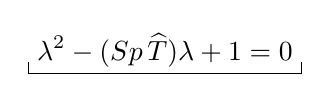
\begin{tikzpicture}[baseline=(eq.base)]
\node[inner xsep=3pt,inner ysep=2pt] (eq) {$\displaystyle
\lambda^2-(Sp\,\widehat T)\lambda+1=0$};
\draw ([yshift=4pt]eq.south west) -- (eq.south west) -- (eq.south east)
      -- ([yshift=4pt]eq.south east);
\end{tikzpicture}}\endgroup
\]


\Needspace{7\baselineskip}
\begin{GelfandAdjacentEvidence}{GELFAND-P000560}{1}
\SourcePage{GELFAND-P000560}{unlabelled}
\sout{Roots}
\Unclear{GELFAND-P000560}{top-old}{The crossed-out word provisionally reads “Roots”. Crossing strokes obscure some letters.}
\end{GelfandAdjacentEvidence}
\begin{GelfandAdjacentEvidence}{GELFAND-P000560}{2}

\begin{gather*}
|\alpha_{11}+\alpha_{22}|<2\quad\Rightarrow\quad\text{complex roots.}\\
|\alpha_{11}+\alpha_{22}|>2\quad\Rightarrow\quad\text{real roots.}
\end{gather*}
The roots run in one direction (can be proved).

\underline{Phys. interpret.}: if there is a bounded eigenfunc., the particle will pass through, if not, it will \sout{not} \fbox{\strut get trapped}
\Unclear{GELFAND-P000560}{trapped-old}{The short crossed-out word before the boxed word provisionally reads “not”.}
\end{GelfandAdjacentEvidence}
\begin{GelfandAdjacentEvidence}{GELFAND-P000560}{3}

\SourceFigure{GELFAND-P000560}{particle-wave}{%
\par\smallskip
\begingroup\color{black}\GelfandFitDiagram{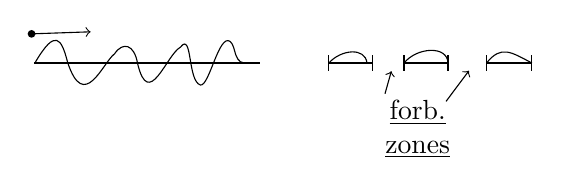
\begin{tikzpicture}[x=.62cm,y=.65cm,every node/.style={inner sep=1pt}]
\draw (0,0) -- (4.62,0);
\fill (-.06,.57) circle (1.4pt);
\draw[->] (-.06,.57) -- (1.15,.61);
\draw (.02,.02) .. controls (.43,.68) and (.55,.49) .. (.68,.01)
  .. controls (1.02,-.97) and (1.40,.01) .. (1.64,.18)
  .. controls (1.81,.42) and (2.04,.37) .. (2.11,0)
  .. controls (2.34,-.94) and (2.70,.16) .. (2.99,.31)
  .. controls (3.24,.62) and (3.13,-.35) .. (3.40,-.43)
  .. controls (3.58,-.46) and (3.78,.59) .. (4.01,.42)
  .. controls (4.15,.31) and (4.05,-.06) .. (4.42,0);
\foreach \xa/\xb in {6.03/6.93,7.57/8.47,9.26/10.19} {
  \draw (\xa,0) -- (\xb,0);
  \draw (\xa,-.15) -- (\xa,.15) (\xb,-.15) -- (\xb,.15);
}
\draw (6.03,0) .. controls (6.28,.27) and (6.78,.31) .. (6.81,0);
\draw (7.57,0) .. controls (7.83,.31) and (8.46,.35) .. (8.47,0);
\draw (9.26,0) .. controls (9.56,.36) and (9.77,.21) .. (10.19,0);
\draw[->] (7.18,-.60) -- (7.31,-.16);
\draw[->] (8.43,-.75) -- (8.90,-.15);
\node[below,align=center] at (7.85,-.67) {\underline{forb.}\\\underline{zones}};
\end{tikzpicture}}\endgroup\par}
\end{GelfandAdjacentEvidence}
\begin{GelfandAdjacentEvidence}{GELFAND-P000560}{4}

\uwave{exp decrease forb. zones}. \hfill (resonance of particle and field)\par
\Unclear{GELFAND-P000560}{decay-old}{At the start of the Russian word for “decrease”, there is a high stroke above overwritten marks. The earlier spelling is illegible.}
\end{GelfandAdjacentEvidence}
\begin{GelfandAdjacentEvidence}{GELFAND-P000560}{5}

\uwave{Ince, Akhiezer, Hochstadt}.
\[
\text{\uwave{Bloch func.}}\;-\;
\boxed{u(x+T)=\nu u(x)},\qquad |\nu|=1.\quad
(\text{eigenvector }\widehat T).
\]
\[
\nu=e^{ip},\qquad p\text{ — “quasimomentum”}.
\]
Bounded eigenfuncs. — if \(p\in\mathbb R\).
\SourceFigure{GELFAND-P000560}{band-lines}{%
\par\smallskip
\begingroup\color{black}\GelfandFitDiagram{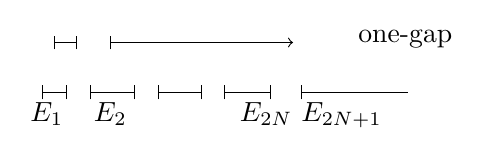
\begin{tikzpicture}[x=.71cm,y=.72cm,every node/.style={inner sep=1pt}]
\draw (.22,0) -- (.60,0);
\draw[->] (1.21,0) -- (4.48,0);
\foreach \x in {.22,.60,1.21}
  \draw (\x,-.12) -- (\x,.12);
\node[anchor=west] at (5.59,.06) {\uwave{one-gap}};
\begin{scope}[yshift=-.63cm]
\draw (0,0) -- (.43,0) (.86,0) -- (1.65,0) (2.08,0) -- (2.85,0)
      (3.26,0) -- (4.07,0) (4.63,0) -- (6.53,0);
\foreach \x in {0,.43,.86,1.65,2.08,2.85,3.26,4.07,4.63}
  \draw (\x,-.13) -- (\x,.13);
\node[below left,inner sep=1pt] at (.43,-.13) {$E_1$};
\node[below right,inner sep=1pt] at (.86,-.13) {$E_2$};
\node[below] at (4.00,-.13) {$E_{2N}$};
\node[below right] at (4.57,-.13) {$E_{2N+1}$};
\end{scope}
\end{tikzpicture}}\endgroup\par}
\end{GelfandAdjacentEvidence}
\begin{GelfandAdjacentEvidence}{GELFAND-P000560}{6}

\[
\Gamma_N\text{ — Riemann surface of }\sqrt{R(E)},\qquad
\text{where}\quad R(E)=\prod_1^{2N+1}(E-E_i)
\]
\uuline{G}. Let \(y(x,E)\) — Bloch func. for complex \(E\).
\[
y(x+T)=\nu y(x)
\]
\(y(x_0,x,E)\)\qquad normalization: \underline{\(y(x_0,x_0,E)=1\)}.
\SourceFigure{GELFAND-P000560}{complex-loop}{%
\par\smallskip
\begingroup\color{black}\GelfandFitDiagram{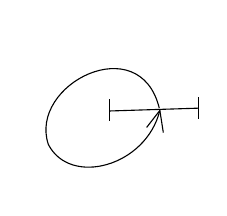
\begin{tikzpicture}[x=.73cm,y=.72cm]
\draw (.99,.04) -- (2.54,.09);
\draw (.99,-.13) -- (.99,.25) (2.54,-.10) -- (2.54,.29);
\draw (1.86,.09) .. controls (1.52,1.50) and (-.42,.51) .. (-.07,-.55)
  .. controls (.31,-1.30) and (1.63,-.94) .. (1.87,.05);
\draw (1.64,-.25) -- (1.87,.05) -- (1.93,-.34);
\end{tikzpicture}}\endgroup\par
Two short diverging strokes are visible where the loop meets the segment. The mark provisionally points upward.}
\end{GelfandAdjacentEvidence}
\begin{GelfandAdjacentEvidence}{GELFAND-P000560}{7}


\uuline{D}.\quad\uuline{Th.~1.} Bloch eigenfuncs. continue analyt. to \(\Gamma_N\).

\uuline{Th.~0}. Any finite-gap pot. — a stat. soln. of a higher KdV eq..

\uuline{Th.~2} The set of pots. with a given spectrum is \(J(\Gamma_N)\) — the Jacobi manifold.
\Unclear{GELFAND-P000560}{manifold-overwrite}{In the Russian abbreviation for “set”, the letter after the hyphen was written over. The earlier strokes are illegible.}
\end{GelfandAdjacentEvidence}
\begin{GelfandAdjacentEvidence}{GELFAND-P000560}{8}

KdV (dyn. syst.) and its higher analogues act there.

On solns. \uwave{\mbox{$Ly=Ey$}} acts \((\widehat Ty)(x)=y(x+T)\)
\[
\begin{aligned}
c&=1,\quad c'=0\\
s&=0,\quad s'=1
\end{aligned}
\qquad(\text{at pt. }x_0)\qquad c(x,x_0,E)
\]
In this basis the monodromy matr. \underline{\(\alpha_{ij}(E,x_0)\)}.

Everything is det. by the matr. trace \(\tau=\frac12 Sp\,\alpha_{ij}\)
\[
|\tau|\le1\quad\Rightarrow\quad\text{\underline{spectral} bands}
\]
\Unclear{GELFAND-P000560}{band-word}{The ending of the Russian word for “bands” is overwritten. The earlier strokes are illegible.}
\end{GelfandAdjacentEvidence}
\begin{GelfandAdjacentEvidence}{GELFAND-P000560}{9}

\[
\tau\text{ is indep. of }x_0,\qquad \underline{\tau=\tau(E)}.
\]
\[
\begingroup\color{black}\GelfandFitDiagram{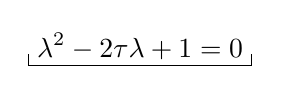
\begin{tikzpicture}[baseline=(eq.base)]
\node[inner xsep=3pt,inner ysep=2pt] (eq)
  {$\displaystyle\lambda^2-2\tau\lambda+1=0$};
\draw ([yshift=4pt]eq.south west) -- (eq.south west) -- (eq.south east)
      -- ([yshift=4pt]eq.south east);
\end{tikzpicture}}\endgroup
\]
\SourceFigure{GELFAND-P000560}{trace-graph}{%
\par\smallskip
\begingroup\color{black}\GelfandFitDiagram{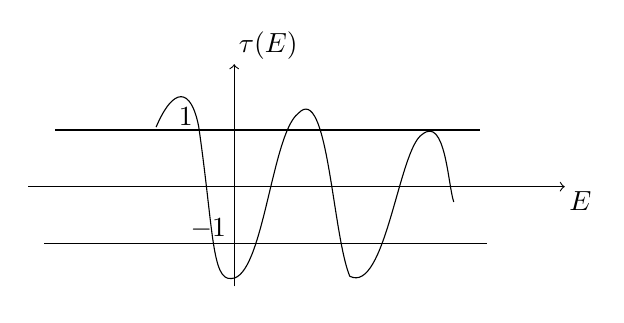
\begin{tikzpicture}[x=.82cm,y=.72cm,every node/.style={inner sep=1.5pt}]
\draw[->] (-3.19,0) -- (5.12,0) node[below right] {$E$};
\draw[->] (0,-1.76) -- (0,2.16) node[above right] {$\tau(E)$};
\draw (-2.77,1) -- (3.81,1);
\draw (-2.94,-1) -- (3.91,-1);
\node[above] at (-.75,1) {$1$};
\node[above] at (-.40,-1) {$-1$};
\draw (-1.21,1.05) .. controls (-.94,1.77) and (-.67,1.76) .. (-.55,1.06)
  .. controls (-.32,-.75) and (-.35,-1.67) .. (-.04,-1.62)
  .. controls (.45,-1.60) and (.58,.93) .. (.99,1.29)
  .. controls (1.45,1.86) and (1.52,-.84) .. (1.79,-1.58)
  .. controls (2.34,-1.90) and (2.55,.66) .. (2.91,.92)
  .. controls (3.27,1.26) and (3.31,.04) .. (3.40,-.27);
\end{tikzpicture}}\endgroup\par}
\end{GelfandAdjacentEvidence}
\begin{GelfandAdjacentEvidence}{GELFAND-P000560}{10}

it is known that the graph looks like this — \uwave{\mbox{$max$} and \mbox{$min\geqslant1$}} — \uwave{prob.}
\Unclear{GELFAND-P000560}{extrema-boundary}{The sign before \(1\) consists of an upper stroke and two oblique strokes. The provisional reading is \(\geqslant\).}
\end{GelfandAdjacentEvidence}



\Needspace{7\baselineskip}
\begin{GelfandAdjacentEvidence}{GELFAND-P000561}{1}
\SourcePage{GELFAND-P000561}{unlabelled}
\uwave{for the \mbox{$2^{*}$} year} \quad There are always infinitely many of them (\underline{\(max\) and \(min\)}).
\Unclear{GELFAND-P000561}{course-ordinal}{A small crossed mark follows “2”. The visible shape is retained. The ending remains unresolved.}
\end{GelfandAdjacentEvidence}
\begin{GelfandAdjacentEvidence}{GELFAND-P000561}{2}

merger of 2 forb. zones — there is no allowed zone
\SourceFigure{GELFAND-P000561}{touching-maxima}{%
\par\smallskip
\begingroup\color{black}\GelfandFitDiagram{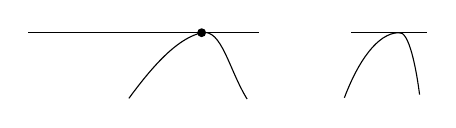
\begin{tikzpicture}[x=.77cm,y=.81cm]
\draw (0,0) -- (3.80,0);
\draw (1.66,-1.03) .. controls (2.16,-.38) and (2.52,-.08) .. (2.86,0)
  .. controls (3.19,.07) and (3.31,-.58) .. (3.61,-1.04);
\fill (2.86,0) circle (1.6pt);
\begin{scope}[xshift=4.1cm]
\draw (0,0) -- (1.26,0);
\draw (-.11,-1.02) .. controls (.12,-.44) and (.44,-.01) .. (.78,0)
  .. controls (.96,.05) and (1.08,-.60) .. (1.13,-.97);
\end{scope}
\end{tikzpicture}}\endgroup\par}
\end{GelfandAdjacentEvidence}
\begin{GelfandAdjacentEvidence}{GELFAND-P000561}{3}

From the eq. \underline{\(\tau(E)=\pm1\)} one must select the \uuline{simple} roots to det. the band edges.

\underline{The band edges} \uwave{give a Jordan block}. If diagonal, we get the degenerate case.

See the work of \uuline{Gelfand and Lidskii} (1955) on systems with periodic coeffs..

\uuline{Def.}\quad
\(\Psi(x,x_0,E),\qquad \Psi(x+T)=e^{ip}\Psi(x),\qquad \Psi(x_0)=1.\)

The other is complex conjugate (when \(|\tau(E)|<1\)).
\[
\text{Let}\qquad
\begingroup\color{black}\GelfandFitDiagram{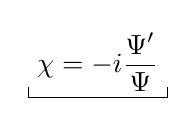
\begin{tikzpicture}[baseline=(eq.base)]
\node[inner xsep=3pt,inner ysep=2pt] (eq)
  {$\displaystyle\chi=-i\frac{\Psi'}{\Psi}$};
\draw ([yshift=4pt]eq.south west) -- (eq.south west) -- (eq.south east)
      -- ([yshift=4pt]eq.south east);
\end{tikzpicture}}\endgroup
\]
1.\quad \(\chi=\chi(x,E)\qquad(\text{indep. of }x_0)\).
\Unclear{GELFAND-P000561}{detached-mark}{A detached “, and” stands to the right between the first and second items. Its attachment remains unclear.}
\end{GelfandAdjacentEvidence}
\begin{GelfandAdjacentEvidence}{GELFAND-P000561}{4}

2.\quad
\begingroup\color{black}\GelfandFitDiagram{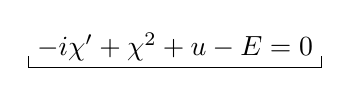
\begin{tikzpicture}[baseline=(eq.base)]
\node[inner xsep=3pt,inner ysep=2pt] (eq) {$-i\chi'+\chi^2+u-E=0$};
\draw ([yshift=4pt]eq.south west) -- (eq.south west) -- (eq.south east)
      -- ([yshift=4pt]eq.south east);
\end{tikzpicture}}\endgroup
\qquad (Riccati eq.).
\[
3.\quad \chi_I=\frac12\frac{\chi_R'}{\chi_R},\qquad
\uwave{\mbox{$\chi=\chi_R+i\chi_I.$}}
\]
\[
4.\quad \chi(x,E)\sim k+\sum_{n=1}^{\infty}\frac{\chi_n(x)}{(2k)^n},
\qquad \text{where } k=\sqrt E
\]
\Unclear{GELFAND-P000561}{series-asymptotic-overwrite}{A wavy stroke lies over earlier strokes before \(k\). The reading \(\sim\) is provisional.}
\end{GelfandAdjacentEvidence}
\begin{GelfandAdjacentEvidence}{GELFAND-P000561}{5}

5.\quad \(\chi(x+T)=\chi(x)\). (asympt. expansion).
\[
\uwave{\mbox{$2\Rightarrow3$}},\qquad 2\Rightarrow4
\]
\Incomplete{GELFAND-P000561}{implication-old}{A group of signs after \(2\Rightarrow4\) is heavily crossed out. The surviving strokes are insufficient to read it.}
\end{GelfandAdjacentEvidence}
\begin{GelfandAdjacentEvidence}{GELFAND-P000561}{6}

\Unclear{GELFAND-P000561}{odd-series-prefix}{A short group is crossed out before \(\chi_R\). It provisionally reads \(\chi\) with a subscript, possibly \(R\).}
\end{GelfandAdjacentEvidence}
\begin{GelfandAdjacentEvidence}{GELFAND-P000561}{7}

\[
\chi_R(x,E)=k+\sum_{n=0}^{\infty}\frac{\chi_{2n+1}(x)}{(2k)^{2n+1}}
\]
\[
\Psi=\exp\left(i\int_{x_0}^{x}\chi\,dx\right)
=\sqrt{\frac{\chi_R(x_0)}{\chi_R(x)}}\exp\left(i\int_{x_0}^{x}\chi_R\,dx\right).
\]
\[
1.\quad|\Psi|^2=\frac{\chi_R(x_0)}{\chi_R(x)}
\]
\[
2.\quad p(E)=\int_0^T\chi_R(x,E)\,dx+\pi n
\]
\Unclear{GELFAND-P000561}{phase-addend}{A heavy slanted mark precedes \(\pi n\). A separate factor remains unresolved.}
\end{GelfandAdjacentEvidence}
\begin{GelfandAdjacentEvidence}{GELFAND-P000561}{8}

Express \(\chi\) in terms of the monodromy matr.

\sout{\underline{Th.}}\quad\underline{Lemma}
\Unclear{GELFAND-P000561}{lemma-cancel}{The underlined “Th.” is crossed out. “Lemma” is inserted above and to its right.}
\end{GelfandAdjacentEvidence}
\begin{GelfandAdjacentEvidence}{GELFAND-P000561}{9}

\begin{equation*}
\chi(x,E)=\frac{\sqrt{1-\tau^2(E)}}{\alpha_{21}(E,x)}
+\frac i2\frac{\alpha_{11}(E,x)\alpha_{22}(E,x)}{\alpha_{21}(E,x)}
\tag{1}
\end{equation*}
\Unclear{GELFAND-P000561}{monodromy-numerator}{A separate sign is indistinguishable between \(\alpha_{11}(E,x)\) and \(\alpha_{22}(E,x)\). The groups are typeset side by side.}
\end{GelfandAdjacentEvidence}

\underline{Proof.}\quad \(\Psi(x,x_0,E)\) — an eigenvector of the monodr. matr. Use the rules of lin. algebra:
\[
\Psi(x,x_0,E)=c(x,x_0,E)+
i\left(\begin{gathered}\text{right-hand side of}\\\text{formula (1) at pt. }x_0\end{gathered}\right)s(x,x_0,E).
\]


\Needspace{7\baselineskip}
\begin{GelfandAdjacentEvidence}{GELFAND-P000562}{1}
\SourcePage{GELFAND-P000562}{unlabelled}
Find the Wronskian det. of this func. and \(c\) (it is indep. of \(x\)).
\begin{gather*}
\left.\{c,\Psi(x,x_0,E)\}\right|_{x_0}=\qquad\text{everything works out.}\\
i\chi(x_0,E)=i(\ldots)\\
\left.\{c,\Psi\}\right|_{x_0}=i\Psi'(x_0)=i\chi(x_0).
\end{gather*}
\Unclear{GELFAND-P000562}{wronskian-overwrite}{An overwritten mark with a prime follows \(i\). The current reading \(\Psi'\) is provisional.}
\end{GelfandAdjacentEvidence}
\begin{GelfandAdjacentEvidence}{GELFAND-P000562}{2}

\SourceFigure{GELFAND-P000562}{degenerate-trace}{%
\par\smallskip
\begingroup\color{black}\GelfandFitDiagram{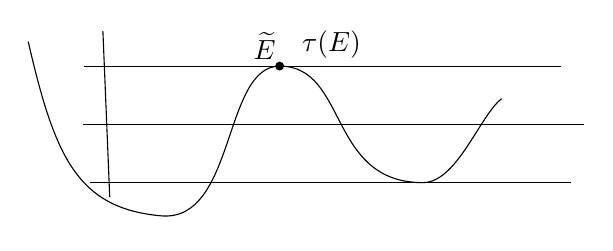
\begin{tikzpicture}[x=.87cm,y=.74cm,every node/.style={inner sep=1pt}]
\draw (-2.18,1) -- (4.78,1) (-2.20,0) -- (5.12,0)
      (-2.10,-1) -- (4.92,-1);
\draw (-1.91,1.60) -- (-1.81,-1.25);
\draw (-3.00,1.42) .. controls (-2.61,-.57) and (-2.28,-1.44) .. (-1.06,-1.57)
  .. controls (.03,-1.68) and (-.16,1) .. (.67,1)
  .. controls (1.67,1) and (1.37,-1) .. (2.76,-1)
  .. controls (3.26,-1) and (3.59,.15) .. (3.91,.44);
\fill (.67,1) circle (1.6pt);
\node[above left] at (.66,1.05) {$\widetilde E$};
\node[above right] at (.95,1.08) {$\tau(E)$};
\end{tikzpicture}}\endgroup\par}
\end{GelfandAdjacentEvidence}
\begin{GelfandAdjacentEvidence}{GELFAND-P000562}{3}

If \((1-\tau(E))\) has a multiple zero, then the monodromy matr. is diagonal, i.e.
\Unclear{GELFAND-P000562}{diagonal-prefix-old}{A short mark resembling “π” is crossed out before the equalities. Its reading remains unresolved.}
\end{GelfandAdjacentEvidence}
\begin{GelfandAdjacentEvidence}{GELFAND-P000562}{4}

\[
\uwave{\mbox{$\alpha_{12}(\widetilde E,x_0)=0,\qquad
             \alpha_{21}(\widetilde E,x_0)=0.$}}
\]
\[
\frac{1-\tau^2(E)}{R(E)}\quad\text{\uwave{has only double degen. zeros}.}
\]
\Unclear{GELFAND-P000562}{quotient-old}{An oblique stroke and an upper line are heavily crossed out to the left of and above the fraction. They may be a deleted radical sign.}
\end{GelfandAdjacentEvidence}
\begin{GelfandAdjacentEvidence}{GELFAND-P000562}{5}

\[
\sqrt{\frac{1-\tau^2(E)}{R(E)}}\quad
\text{\uwave{has only simple zeros}.}\qquad(\text{see Titchmarsh})
\]
\underline{\(\alpha_{21}(\widetilde E,x_0)=0\)} \underline{too}
\[
\uwave{\mbox{$\displaystyle\alpha_{21}=\widetilde\alpha_{21}\cdot
\sqrt{\frac{1-\tau^2(E)}{R(E)}}$}}\qquad(\text{divided}).
\]
Substitute into the formula for \(\chi_R\):
\[
\chi_R=\frac{\sqrt{R(E)}}{\widetilde\alpha_{21}(E,x)},
\qquad\text{where }\widetilde\alpha_{21}(E,x)\text{ — an entire anal. func. of }E.
\]
\[
\chi_R=k+O\left(\frac1k\right),\qquad
\sqrt{R(E)}\sim E^N\quad\text{at infinity}.
\]
\Unclear{GELFAND-P000562}{infinity-power}{The visible exponent in this line is \(N\). The numerator in the next line is \(kE^N\).}
\end{GelfandAdjacentEvidence}
\begin{GelfandAdjacentEvidence}{GELFAND-P000562}{6}

\[
\chi_R(x,E)\sim\frac{kE^N}{E^N}\quad\Rightarrow\quad
\widetilde\alpha_{21}(E,x)\text{ — a polynomial in }E.
\]
\hfill\uwave{\mbox{$P(E,x)$}}\par
\(\chi_R(x,E)\) — 2-valued analyt. func. (analyt. continuation from real \(E\) in a band)
\[
\chi_R(x,E)=\frac{\sqrt{R(E)}}{P(E,x)}
\]
\[
P(E,x)=\prod(E-\gamma_i(x)),\qquad
\gamma_i(x)\text{ — roots of the polynomial}
\]
\[
\text{Hence}:\quad
\boxed{\chi(x,E)=\left(\sqrt R-\frac i2\frac d{dx}P\right)/P.}
\]
\[
\chi_R\sim k+\sum\frac{\chi_{2n+1}(x)}{(2k)^{2n+1}}
\]
\Unclear{GELFAND-P000562}{odd-index}{The letter \(n\) in the subscript \(2n+1\) has been written over. The earlier strokes are illegible.}
\end{GelfandAdjacentEvidence}

Construct the functionals
\[
I_n\{u\}=\int_0^T\chi_{2n+3}(x)\,dx
\]


\Needspace{7\baselineskip}
\begin{GelfandAdjacentEvidence}{GELFAND-P000563}{1}
\SourcePage{GELFAND-P000563}{unlabelled}
\[
\begingroup\color{black}\GelfandFitDiagram{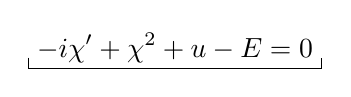
\begin{tikzpicture}[baseline=(eq.base)]
\node[inner xsep=3pt,inner ysep=2pt] (eq) {$\displaystyle-i\chi'+\chi^2+u-E=0$};
\draw ([yshift=4pt]eq.south west) -- (eq.south west) -- (eq.south east)
      -- ([yshift=4pt]eq.south east);
\end{tikzpicture}}\endgroup
\quad\Rightarrow\quad\text{asymptotics}.
\]
and in this case \(\chi_{2n+1}=Q(u,u',\ldots,u^{(n-1)})\) — \uwave{a polynomial}.
\Unclear{GELFAND-P000563}{derivative-order}{The order above the last \(u\) provisionally reads \((n-1)\).}
\end{GelfandAdjacentEvidence}
\begin{GelfandAdjacentEvidence}{GELFAND-P000563}{2}

\Unclear{GELFAND-P000563}{left-old-symbol}{A group with vertical strokes and a loop is crossed out at the left. The visible sign resembles “δ” or “\(\int\)”. The earlier writing remains unresolved.}
\end{GelfandAdjacentEvidence}
\begin{GelfandAdjacentEvidence}{GELFAND-P000563}{3}

\sout{This […]}
\Unclear{GELFAND-P000563}{stationary-fragment}{The beginning of the crossed-out line provisionally reads “This”.}
\end{GelfandAdjacentEvidence}
\begin{GelfandAdjacentEvidence}{GELFAND-P000563}{4}

\Incomplete{GELFAND-P000563}{stationary-old}{The remaining words in the crossed-out line are illegible.}
\end{GelfandAdjacentEvidence}

\[
\frac{\delta}{\delta u}\left\{\sum c_n I_n\right\}=d\quad(=const).
\]
\noindent\(\cdot\quad\cdot\quad\cdot\quad\cdot\quad\cdot\quad\cdot\quad\cdot
\quad\cdot\quad\cdot\quad\cdot\quad\cdot\quad\cdot\quad\cdot\)


\Needspace{7\baselineskip}
\begin{GelfandAdjacentEvidence}{GELFAND-P000564}{1}
\SourcePage{GELFAND-P000564}{unlabelled}
\noindent\hfill\rule{1.35cm}{.28pt}\enspace\rule{.55cm}{.40pt}\hfill\mbox{}\par
\uwave{\mbox{$23/\underline{\overline{\mathrm{IX}}}-74$}}\qquad\uuline{Gelfand Sem.}

On the work of \uwave{Gabrielov, I. Gelfand and Losik} on combinatorial topology.

It is interesting to do it analytically.
\sout{\mbox{$\int$} […]}
\Unclear{GELFAND-P000564}{analytic-fragment}{A mark with two loops begins the crossed-out group. It provisionally reads \(\int\).}
\end{GelfandAdjacentEvidence}
\begin{GelfandAdjacentEvidence}{GELFAND-P000564}{2}

\Incomplete{GELFAND-P000564}{analytic-old}{Oblique strokes obscure the remaining marks. They are illegible.}
\end{GelfandAdjacentEvidence}
\begin{GelfandAdjacentEvidence}{GELFAND-P000564}{3}

\[
\int_{1-x}^{x}\left[\frac{\log|t|}{1-t}+\frac{\log|1-t|}{t}\right]\,dt
\]
cannot be evaluated in elem. funcs.. But:
\[
\int_0^1\frac{\log|1-t|}{t}\,dt=\frac{\pi^2}{6}
\quad\left(=\int_0^1\sum_{n=1}^{\infty}\frac{t^{n-1}}n
=\sum_{n=1}^{\infty}\frac1{n^2}\right).
\]
\Unclear{GELFAND-P000564}{integral-sign}{There is no minus sign before \(\pi^2/6\). The middle term has no written differential.}
\end{GelfandAdjacentEvidence}
\begin{GelfandAdjacentEvidence}{GELFAND-P000564}{4}

One can evaluate
\[
\int_{2-\sqrt5}^{\sqrt5-2}\left[\frac{\log|t|}{1-t}+\frac{\log|1-t|}{t}\right]\,dt
=-\frac{\pi^2}{6}
\]
\Unclear{GELFAND-P000564}{symmetric-integral}{This line shows a minus sign before \(\pi^2/6\). The limits read \(2-\sqrt5\) and \(\sqrt5-2\).}
\end{GelfandAdjacentEvidence}
\begin{GelfandAdjacentEvidence}{GELFAND-P000564}{5}

(from topological considerations).
\Unclear{GELFAND-P000564}{topological-overwrite}{Both Russian words contain overwritten letters. The earlier strokes are illegible.}
\end{GelfandAdjacentEvidence}
\begin{GelfandAdjacentEvidence}{GELFAND-P000564}{6}

They occur in a finite combinatorial problem.

\uwave{Graeme Segal} — all of topology.

\uuline{Giusti.} On singularities. (On regularity of \sout{[…]} solv. of nonlin. syst.).
\Unclear{GELFAND-P000564}{speaker-name}{The name in the Russian handwriting provisionally reads “Джусти”. The middle strokes run together.}
\end{GelfandAdjacentEvidence}
\begin{GelfandAdjacentEvidence}{GELFAND-P000564}{7}

\Incomplete{GELFAND-P000564}{regularity-old}{A short entry before “solv.” in the English parenthesis is heavily crossed out and illegible.}
\end{GelfandAdjacentEvidence}
\begin{GelfandAdjacentEvidence}{GELFAND-P000564}{8}

\uwave{Symplest case}:
\[
\sum_{i,j=1}^{n}\sum_{h,k=1}^{N}\int a_{ij}^{hk}(x,u)D_i u^h D_j\varphi^k\,dx=0
\]
\Unclear{GELFAND-P000564}{weak-overwrites}{There are overwritten marks in the argument \((x,u)\) and before the superscript \(k\). The current readings \(u\) and \(\varphi\) are provisional.}
\end{GelfandAdjacentEvidence}
\begin{GelfandAdjacentEvidence}{GELFAND-P000564}{9}

\[
D_i=\frac\partial{\partial x},\qquad
\forall\varphi=(\varphi^1,\ldots,\varphi^N),\qquad
\varphi_i\in W_0^{1,2}(\Omega)
\]
\Unclear{GELFAND-P000564}{test-component-old}{There is a heavy subscript mark below \(\varphi^1\). It may be \(2\), \(i\) or \(z\). Its reading remains unresolved.}
\end{GelfandAdjacentEvidence}
\begin{GelfandAdjacentEvidence}{GELFAND-P000564}{10}

\[
\sum_{i,j=1}^{n}\sum_{h=1}^{N}D_j\bigl(a_{ij}^{hk}(x,u)D_i u^k\bigr)=0
\qquad(k=1,2,\ldots,N)
\]
\Unclear{GELFAND-P000564}{system-indices}{The written denominator of \(D_i\) is \(\partial x\). In the sum over \(h\) the visible superscript of \(u\) is \(k\).}
\end{GelfandAdjacentEvidence}
\begin{GelfandAdjacentEvidence}{GELFAND-P000564}{11}

\[
u=(u^1,\ldots,u^N).
\]
\uwave{Ellipticity}:
\[
\sum_{ijhk}a_{ij}^{hk}(x,t)\xi_i^h\xi_j^k\geqslant|\xi|^2,\qquad
\forall x\in\Omega,\ \forall t\in\mathbb R^n
\]
\Unclear{GELFAND-P000564}{ellipticity-indices}{The first subscript on \(\xi\) provisionally reads \(i\). The final dimension reads \(n\).}
\end{GelfandAdjacentEvidence}



\Needspace{7\baselineskip}
\begin{GelfandAdjacentEvidence}{GELFAND-P000565}{1}
\SourcePage{GELFAND-P000565}{unlabelled}
\[
\sum_{i,j=1}^{n}D_j\bigl(A_{ij}(x,u)D_i u\bigr)=0,
\qquad\begin{gathered}
u\text{ — a vector}\\
A_{ij}\text{ — a matrix}.
\end{gathered}
\]
\underline{\(N=1\)} \(\ \Rightarrow\forall\) solution is regular

or \underline{\(n\leqslant2\)}\qquad
\(\forall u\in W^{1,1}\) is regular (depende on reg. of \(A\)-coefficients)
\Unclear{GELFAND-P000565}{dimension-overwrite}{The sign between \(n\) and \(2\) has been written over. The current reading \(\leqslant\) is provisional.}
\end{GelfandAdjacentEvidence}
\begin{GelfandAdjacentEvidence}{GELFAND-P000565}{2}

\Unclear{GELFAND-P000565}{coefficient-old}{The mark before “coefficients” has been written over. It provisionally reads “A”. The earlier strokes are illegible.}
\end{GelfandAdjacentEvidence}
\begin{GelfandAdjacentEvidence}{GELFAND-P000565}{3}

\[
A\in C^\infty\quad\Rightarrow\quad u\in C^\infty\quad\text{etc.}
\]
\begin{gather*}
W^{1,2},\qquad u\in L_2,\qquad \int_{\Omega}|Du|^2\,dx<+\infty\\
W_0^{1,2}\text{ — 0 boundary values.}
\end{gather*}
\Unclear{GELFAND-P000565}{boundary-overwrite}{The “d” in “boundary” has been written over. Above the word, \(\Omega\) is below the integral in the previous line.}
\end{GelfandAdjacentEvidence}
\begin{GelfandAdjacentEvidence}{GELFAND-P000565}{4}

\(n=\)\underline{\(N\geqslant3\)}\qquad\uwave{falls}.
\Unclear{GELFAND-P000565}{dimension-three}{The digit “3” has been written over. The earlier strokes beneath it remain unresolved.}
\end{GelfandAdjacentEvidence}
\begin{GelfandAdjacentEvidence}{GELFAND-P000565}{5}

\Unclear{GELFAND-P000565}{fails-spelling}{The English word has two tall loops with no dot over the first. It is transcribed as “falls”.}
\end{GelfandAdjacentEvidence}
\begin{GelfandAdjacentEvidence}{GELFAND-P000565}{6}

\[
a_{ij}^{hk}=\delta_{ij}\delta_{hk}+
\left(\delta_{jk}+\frac1{n-2}\frac{u_j u_k}{1+|u|^2}\right)
\left(\delta_{ih}+\frac4{n-2}\frac{u_i u_h}{1+|u|^2}\right)
\]
\Unclear{GELFAND-P000565}{coefficient-formula}{The written factors preceding the fractions are \(1/(n-2)\) and \(4/(n-2)\), in that order.}
\end{GelfandAdjacentEvidence}
\begin{GelfandAdjacentEvidence}{GELFAND-P000565}{7}

\uwave{\mbox{$u_i=x_i/|x|$}} — \uwave{solution}.
\qquad\uwave{coefficients are real analityc}
\Unclear{GELFAND-P000565}{source-english-spelling}{The original English spelling “analityc” is retained.}
\end{GelfandAdjacentEvidence}
\begin{GelfandAdjacentEvidence}{GELFAND-P000565}{8}

\underline{\(n=2\)}\qquad \(\forall\) sol. is regular

\underline{\(n=3,\ N=2\)} — there is an example of non regular solution.

\uwave{For Dirichlet problem}. \(u_i=x_i\) when \(|x|=1\).
\(\exists!\) solution and it is not regular!

\noindent\hfill\rule{1.1cm}{.32pt}\enspace\(\cdot\)\enspace\rule{.9cm}{.32pt}\par
Suppose \(a_{ij}^{hk}\) are \uwave{continuous}

Then (1) \(\forall\) solution \(u\) of system is regular in an open set \(\Omega_0\subset\Omega\)
\Unclear{GELFAND-P000565}{old-number}{An entry in parentheses is crossed out before “(2)”. The earlier number is illegible.}
\end{GelfandAdjacentEvidence}
\begin{GelfandAdjacentEvidence}{GELFAND-P000565}{9}

(2). \(K=\Omega-\Omega_0\) (\(K\) is closed in \(\Omega\)) \sout{a[…]}
\[
\Rightarrow\underset{H_{n-2}}{\mathrm{meas}} K=0
\]
\Unclear{GELFAND-P000565}{old-at}{An initial “a” is visible in the crossed-out English word. The remaining letters are unresolved.}
\end{GelfandAdjacentEvidence}
\begin{GelfandAdjacentEvidence}{GELFAND-P000565}{10}

\[
\uwave{\mbox{$\dim K<n-2.$}}
\]
\Unclear{GELFAND-P000565}{hausdorff-sign}{The lower stroke of the sign in the \(\dim K\) line is thickened. The visible outline is transcribed as \(<\).}
\end{GelfandAdjacentEvidence}
\begin{GelfandAdjacentEvidence}{GELFAND-P000565}{11}

(for order \(m>2\qquad\dim K\leqslant n-2\)).

\noindent\hfill\rule{1.1cm}{.32pt}\enspace\(\cdot\)\enspace\rule{.9cm}{.32pt}\par
\sout{There} Are \sout{also} [inserted above] there variational problems with nonregular solutions?
\Unclear{GELFAND-P000565}{variational-old}{The crossed-out words before and after “Are” provisionally read “There” and “also”. The inserted “there” is enclosed above the line.}
\end{GelfandAdjacentEvidence}

\noindent\hfill\rule{1.1cm}{.32pt}\enspace\(\cdot\)\enspace\rule{.9cm}{.32pt}\par
\uuline{Problem of Gelfand}. Devise an analogue of Hironaka’s resol. of sing. for elliptic eqs..


\Needspace{7\baselineskip}
\begin{GelfandAdjacentEvidence}{GELFAND-P000566}{1}
\SourcePage{GELFAND-P000566}{unlabelled}
\uwave{I. M. Gelfand}\qquad recap of Dubrovin’s previous talk.
\SourceFigure{GELFAND-P000566}{heading-capped-separator}{%
\par\smallskip
\begingroup\color{black}\GelfandFitDiagram{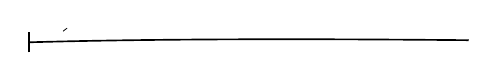
\begin{tikzpicture}[x=.75cm,y=.67cm]
\draw[line width=.6pt] (0,0) .. controls (2.5,.08) and (5.5,.06) .. (7.45,.04);
\draw[line width=.8pt] (0,-.19) -- (0,.20);
\draw[line width=.28pt] (.58,.21) -- (.65,.27);
\end{tikzpicture}}\endgroup\par
There is a small detached slanted stroke above the left end.}
\end{GelfandAdjacentEvidence}
\begin{GelfandAdjacentEvidence}{GELFAND-P000566}{2}

\begin{gather*}
-y''+u(x)y=Ey\\
u(x+T)=u(y)
\end{gather*}
\Unclear{GELFAND-P000566}{period-argument}{The right-hand side clearly reads \(u(y)\).}
\end{GelfandAdjacentEvidence}
\begin{GelfandAdjacentEvidence}{GELFAND-P000566}{3}

The spectrum — those \(E\), for which there are bounded eigenfuncs.
\Unclear{GELFAND-P000566}{energy-overwrites}{Both letters \(E\) are written over with heavy strokes. The earlier signs remain unresolved.}
\end{GelfandAdjacentEvidence}
\begin{GelfandAdjacentEvidence}{GELFAND-P000566}{4}

\uwave{Novikov’s problem}: when are there finitely many forbidden zones?
\SourceFigure{GELFAND-P000566}{spectral-bands}{%
\par\smallskip
\begingroup\color{black}\GelfandFitDiagram{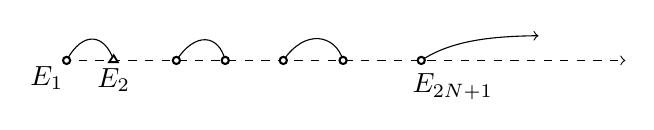
\begin{tikzpicture}[x=.73cm,y=.73cm,every node/.style={inner sep=1pt}]
\draw[dashed,->] (.32,0) -- (10.12,0);
\draw (.40,0) .. controls (.68,.52) and (1.06,.47) .. (1.22,0);
\draw (2.31,0) .. controls (2.64,.51) and (3.05,.45) .. (3.16,0);
\draw (4.17,0) .. controls (4.55,.56) and (5.08,.45) .. (5.21,0);
\draw[->] (6.57,0) .. controls (7.07,.33) and (7.72,.42) .. (8.61,.43);
\foreach \x in {.40,2.31,3.16,4.17,5.21,6.57}
  \draw[line width=.75pt,fill=white] (\x,0) circle (1.3pt);
\draw[line width=.65pt,fill=white] (1.14,-.03) -- (1.29,-.03) -- (1.22,.09) -- cycle;
\node[below left] at (.40,-.05) {$E_1$};
\node[below] at (1.22,-.09) {$E_2$};
\node[below right] at (6.36,-.18) {$E_{2N+1}$};
\end{tikzpicture}}\endgroup\par}
\end{GelfandAdjacentEvidence}
\begin{GelfandAdjacentEvidence}{GELFAND-P000566}{5}

\uuline{Th. Novik.–Dubrov}.
\Unclear{GELFAND-P000566}{theorem-name}{A heavy stroke is written over the end of the abbreviated name “Dubrov.” The earlier letter remains unresolved.}
\end{GelfandAdjacentEvidence}
\begin{GelfandAdjacentEvidence}{GELFAND-P000566}{6}

These are the potentials \(\Leftrightarrow\) satisf. the nonlin. eq.
\[
K(u,u',\ldots,u^{(2N)})=0
\]
(Higher Korteweg–de Vries eq.)
\begin{align*}
c(x,x_0,E)&:\qquad c(x_0)=1,\quad c'(x_0)=0\\
s(x,x_0,E)&:\qquad s(x_0)=0,\quad s'(x_0)=1.
\end{align*}
These are analyt. funcs. of the parameter \(E\).
\[
\widehat T\Psi=\Psi(x+T),\qquad
\widehat T=\begin{pmatrix}\alpha_{11}&\alpha_{12}\\
                           \alpha_{21}&\alpha_{22}\end{pmatrix}
\qquad\det\|\widehat T\|=1.
\]
Bloch func.: \uwave{\mbox{$\Psi(x+T)=\lambda\Psi(x)$}},\qquad \(\Psi(x_0)=1\)

This is an eigenvector for \(\widehat T\).
\begin{gather*}
\lambda^2-(\alpha_{11}+\alpha_{22})\lambda+1=0,\\
\lambda^2-2\tau\lambda+1=0,\qquad
\tau(E)=\frac{\alpha_{11}+\alpha_{22}}2.
\end{gather*}
\(E\in\) an allowed interv. \(\Leftrightarrow\exists\) a Bloch func. with \(|\lambda|=1\).

\(\tau^2\leqslant1\) — allowed int., \(\tau^2>1\) — forbidden
\SourceFigure{GELFAND-P000566}{first-trace}{%
\par\smallskip
\begingroup\color{black}\GelfandFitDiagram{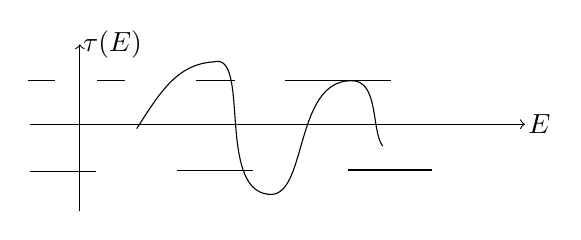
\begin{tikzpicture}[x=.84cm,y=.7cm,every node/.style={inner sep=1pt}]
\draw[->] (-.75,0) -- (6.73,0) node[right] {$E$};
\draw[->] (0,-1.58) -- (0,1.45) node[right] {$\tau(E)$};
\draw (-.78,.79)--(-.37,.79) (.26,.79)--(.68,.79)
      (1.75,.79)--(2.34,.79) (3.10,.79)--(4.70,.79);
\draw (-.75,-.86)--(.24,-.86) (1.47,-.84)--(2.62,-.84)
      (4.06,-.83)--(5.33,-.83);
\draw (.86,-.08) .. controls (1.20,.55) and (1.46,1.09) .. (2.02,1.13)
  .. controls (2.58,1.33) and (2.07,-1.16) .. (2.84,-1.27)
  .. controls (3.45,-1.39) and (3.22,.78) .. (4.10,.79)
  .. controls (4.53,.80) and (4.40,-.11) .. (4.58,-.40);
\end{tikzpicture}}\endgroup\par}
\end{GelfandAdjacentEvidence}
\begin{GelfandAdjacentEvidence}{GELFAND-P000566}{7}

all \(max\geqslant1\qquad\) (this shape).

Correct fig.:
\SourceFigure{GELFAND-P000566}{corrected-trace}{%
\par\smallskip
\begingroup\color{black}\GelfandFitDiagram{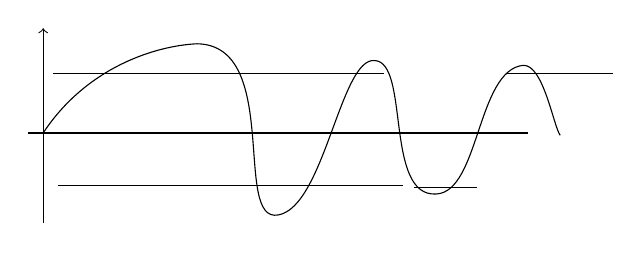
\begin{tikzpicture}[x=.76cm,y=.76cm]
\draw[->] (0,-1.50) -- (0,1.75);
\draw (-.25,0) -- (8.10,0);
\draw (.16,1)--(5.70,1) (7.75,1)--(9.53,1);
\draw (.25,-.88)--(6.02,-.88) (6.19,-.91)--(7.25,-.91);
\draw (0,0) .. controls (.74,1.12) and (1.91,1.46) .. (2.57,1.49)
  .. controls (3.99,1.47) and (3.16,-1.52) .. (3.93,-1.37)
  .. controls (4.70,-1.23) and (4.97,1.27) .. (5.54,1.21)
  .. controls (6.13,1.18) and (5.70,-1.08) .. (6.57,-1.02)
  .. controls (7.29,-.98) and (7.25,1.05) .. (8.02,1.13)
  .. controls (8.36,1.15) and (8.53,.10) .. (8.64,-.04);
\end{tikzpicture}}\endgroup\par}
\end{GelfandAdjacentEvidence}
\begin{GelfandAdjacentEvidence}{GELFAND-P000566}{8}

The forb. zones shrink.

\uline{Important conclusion}: if all the zones have merged, then, \(max\) and \(min\) are equal from some point on to \(1\).

\uwave{They cannot}, since the problem with periodic conds. has infinite spectrum (there \underline{\(\tau=1\)}).
\SourceFigure{GELFAND-P000566}{jordan-extrema}{%
\par\smallskip
\begingroup\color{black}\GelfandFitDiagram{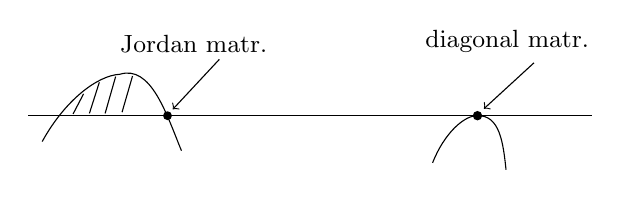
\begin{tikzpicture}[x=.74cm,y=.73cm,every node/.style={inner sep=1pt,font=\small}]
\draw (-.26,0) -- (9.41,0);
\draw (-.02,-.45) .. controls (.37,.27) and (.93,.70) .. (1.31,.72)
  .. controls (1.85,.89) and (2.11,.03) .. (2.37,-.61);
\draw (.51,.03)--(.69,.38) (.79,.04)--(.96,.58)
      (1.06,.04)--(1.24,.68) (1.35,.06)--(1.53,.69);
\draw (6.68,-.82) .. controls (6.88,-.30) and (7.23,.01) .. (7.45,0)
  .. controls (7.83,.01) and (7.89,-.46) .. (7.94,-.94);
\fill (2.13,0) circle (1.6pt) (7.45,0) circle (1.7pt);
\draw[->] (3.02,.98) -- (2.22,.11);
\draw[->] (8.42,.92) -- (7.56,.12);
\node[above] at (2.58,1.04) {Jordan matr.};
\node[above] at (7.96,1.04) {diagonal matr.};
\end{tikzpicture}}\endgroup\par}
\end{GelfandAdjacentEvidence}
\begin{GelfandAdjacentEvidence}{GELFAND-P000566}{9}

(stand. perturbation theory for ordinary eqs.).
\[
\tau^2(E)=1\quad\text{has a mult. root}\quad\Rightarrow\quad\alpha_{12}=\alpha_{21}=0.
\]
\Unclear{GELFAND-P000566}{alpha-index}{The first digit of the subscript on \(\alpha_{12}\) has been written over. The visible reading is \(1\).}
\end{GelfandAdjacentEvidence}
\begin{GelfandAdjacentEvidence}{GELFAND-P000566}{10}

\(\alpha_{12}(E)\) and \(\alpha_{21}(E)\) have a zero at the same points where \(\tau^2(E)-1\) has multiple zeros.

Consid. the Bloch func. \(\Psi(x,x_0,E)\):\qquad \(\Psi(x,x_0,E),\quad\Psi(x_0)=1.\)

there are 2 Bloch funcs. \(\forall E\) (since the eq. is quadr. in \(\lambda\)).

it depends analyt. on \(E\) (two-valued).
\SourceFigure{GELFAND-P000566}{boundary-bands}{%
\par\smallskip
\begingroup\color{black}\GelfandFitDiagram{\begin{tikzpicture}[x=.74cm,y=.72cm]
\draw (0,0)--(1.19,0) (2.17,0)--(3.44,0) (4.30,0)--(5.53,0)
      (7.08,0)--(9.58,0);
\foreach \x in {0,1.19,2.17,3.44,4.30,5.53,7.08}
  \draw (\x,-.16)--(\x,.16);
\end{tikzpicture}}\endgroup\par}
\end{GelfandAdjacentEvidence}

\(\tau^2(E)-1\) has a zero at \(E_1,\ldots,E_{2N+1}\). The rest are double.


\Needspace{7\baselineskip}
\begin{GelfandAdjacentEvidence}{GELFAND-P000567}{1}
\SourcePage{GELFAND-P000567}{unlabelled}
\[
\begingroup\color{black}\GelfandFitDiagram{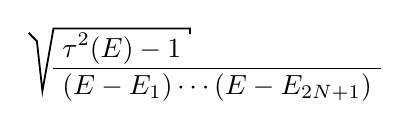
\begin{tikzpicture}[baseline=0pt]
\node[anchor=south west,inner xsep=3pt,inner ysep=1.5pt] (num) at (0,0)
  {$\displaystyle\tau^2(E)-1$};
\node[anchor=north west,inner xsep=3pt,inner ysep=1.5pt] (den) at (0,0)
  {$\displaystyle(E-E_1)\cdots(E-E_{2N+1})$};
\draw (den.north west) -- (den.north east);
\draw[line width=.65pt] (-9pt,13pt)--(-6pt,10pt)--(-4pt,-8pt)
  -- (num.north west) -- (num.north east) -- ([yshift=-2pt]num.north east);
\end{tikzpicture}}\endgroup
\qquad\text{— single-valued func.}
\]
\Unclear{GELFAND-P000567}{root-scope}{The top stroke of the radical ends over the numerator. The bottom of the radical descends to the denominator. Its scope remains ambiguous.}
\end{GelfandAdjacentEvidence}
\begin{GelfandAdjacentEvidence}{GELFAND-P000567}{2}

Consid. the eq.
\begin{gather*}
-\Psi''+u(x)\Psi=E\Psi,\qquad \Psi(x+T)=\lambda\Psi(x)\\
u(x+T)=u(x)
\end{gather*}
Let \(\chi=-i\,\Psi'/\Psi\).

\(1^\circ.\quad \chi\) does not depend on \(x_0,\quad\chi=\chi(x,E)\).

\(2^\circ.\quad \chi(x+T)=\chi(x).\)

\(3^\circ.\quad -i\chi'+\chi^2+u-E=0.\)

\(\chi=\chi_R+i\chi_I\) in an allowed band — then analyt. continuation in \(E\).
\[
4^\circ.\quad\chi_I=\frac12\,\chi_R'/\chi_R.
\]
\begin{gather*}
5^\circ.\quad\chi(x,E)\sim k+\sum_{n=1}^{\infty}\frac{\chi_n(x)}{(2k)^n},
\qquad E=k^2\\
\chi_n=P_n(u,u',\ldots,u^{(n)})\text{ — a polynomial}
\end{gather*}
(det. successively from the asympt. equality)
\[
4^\circ\Rightarrow6^\circ.\quad\chi_R(x,E)\sim k+
\sum_{n=0}^{\infty}\frac{\chi_{2n+1}(x)}{(2k)^{2n+1}}
\]
\[
7^\circ.\quad\Psi(x,x_0,E)=
\sqrt{\frac{\chi_R(x_0,E)}{\chi_R(x,E)}}\cdot
\exp\left[i\int_{x_0}^x\chi_R(t,E)\,dt\right].
\]
\Unclear{GELFAND-P000567}{exponent-overwrites}{The subscript of \(\chi_R\) in the numerator has been written over. In the exponent, \(t\), \(E\) and the final \(t\) of \(dt\) have been written over. The earlier strokes remain unresolved.}
\end{GelfandAdjacentEvidence}
\begin{GelfandAdjacentEvidence}{GELFAND-P000567}{3}

\[
7^\circ\Rightarrow8^\circ.\quad|\Psi|^2=\chi_R(x_0,E)/\chi_R(x,E)
\qquad\text{\uwave{in an allowed band}}
\]
\(9^\circ.\quad\) \sout{[…]}
\Unclear{GELFAND-P000567}{phase-old}{An entry before \(\lambda\) is heavily crossed out. Some strokes resemble an equals sign and \(p(E)\). The exact reading remains unresolved.}
\end{GelfandAdjacentEvidence}
\begin{GelfandAdjacentEvidence}{GELFAND-P000567}{4}

\[
\lambda=e^{ip(E)}\quad\Rightarrow\quad
p(E)=\int_{x_0}^{x_0+T}\chi_R(x,E)\,dx+2\pi n.
\]
The integral — a functional of \(u\) with an \uwave{asympt. expansion}. Its Euler eq. — \uwave{KdV eqs.},

Allowed and forb. zones — where \(|\lambda|=1\)
\Unclear{GELFAND-P000567}{old-ordinal}{An earlier number with a superscript circle is crossed out to the left of “10°”. A vertical stroke and a loop are visible. The exact digits remain unresolved.}
\end{GelfandAdjacentEvidence}
\begin{GelfandAdjacentEvidence}{GELFAND-P000567}{5}

\[
10^\circ.\quad\frac{\delta p(E)}{\delta u(x)}=-\frac12\frac1{\chi_R(x,E)}
\]
(left-hand side of the Euler eq. for KdV).
\[
11^\circ.\quad\chi(x,E)=
\frac{\sqrt{1-\tau^2(E)}}{\alpha_{21}(x,E)}+
\frac i2\frac{\alpha_{11}(x,E)-\alpha_{22}(x,E)}{\alpha_{21}(x,E)}
\]
Rough idea: eigenvalue obtained from the quadr. eq.
\[
12^\circ.\quad\text{Let}\quad R(E)=\prod_1^{2N+1}(E-E_j).
\qquad\text{Then}
\]
\[
\chi(x,E)=\frac{\sqrt{R(E)}}{P(E,x)}-\frac i2\frac{P'_x}{P},
\]
where \(P\) — a polynomial in \(E\) of degree \(N\).
\Unclear{GELFAND-P000567}{polynomial-prime}{A heavy stroke follows \(P'_x\) in the numerator. It resembles an opening parenthesis. Its meaning remains unresolved.}
\end{GelfandAdjacentEvidence}



\Needspace{7\baselineskip}
\begin{GelfandAdjacentEvidence}{GELFAND-P000568}{1}
\SourcePage{GELFAND-P000568}{unlabelled}
\[
P(E,x)=\prod_{j=1}^{N}(E-\gamma_j(x)).
\]
\uuline{G.’s problem.} Let \(R\) and \(P\) — entire funcs. of the 1st order of growth. Then corresponding to them are potentials \(u(x)\). Which ones?

class of potentials (not necessarily periodic).
\noindent\hfill\rule{1.1cm}{.32pt}\enspace\(\cdot\)\enspace\rule{.9cm}{.32pt}\par
\underline{Dubrovin.}

\(\Gamma_N\) — Riem. surf. of \(\sqrt{R(E)}\), \(\chi(x,E)\) — an algebr. func. on this surface

\underline{Theorem}: \(\Psi(x,x_0,E)\) a single-valued func. on \(\Gamma_N\),
merom. on \(\Gamma_N\setminus\infty\), has \(N\) zeros and \(N\) poles.
\Unclear{GELFAND-P000568}{bloch-separator}{A comma follows the first \(x\). A small mark is heavily crossed out above it. The earlier reading remains unresolved.}
\end{GelfandAdjacentEvidence}

Poles at \uwave{\mbox{$E=\gamma_i(x_0)$}},
zeros above \(E=\gamma_i(x)\).


\Needspace{7\baselineskip}
\begin{GelfandAdjacentEvidence}{GELFAND-P000569}{1}
\SourcePage{GELFAND-P000569}{unlabelled}
\uuline{\mbox{$30/\underline{\overline{\mathrm{IX}}}-74$}.}\qquad
\uwave{Gelfand Sem.}

\uuline{Polyakov.}\quad\uwave{On elementary particles.}\quad\uwave{Yang–Mills fields.}
\hfill(difference analogue).\par

\uuline{Graeme Segal.}\qquad\underline{A work of \uuline{Dusa Mc Duff} on config. space.}
\[
\mathbb R^n,\qquad
C_k(\mathbb R^n)=\{\text{subsets of }\mathbb R^n\text{ with }k
\text{ points (no ordered)}\}.
\]
From a top. point of view it is not quite trivial.
\SourceFigure{GELFAND-P000569}{point-axes}{%
\par\smallskip
\begingroup\color{black}\GelfandFitDiagram{\begin{tikzpicture}[x=.80cm,y=.75cm]
\draw (-1.46,-.03)--(1.45,.04);
\draw (1.45,.04)--(1.31,.11) (-1.46,-.03)--(-1.33,-.11);
\draw (0,-.87)--(.02,1.47);
\draw[line width=.70pt] (-.92,.91) circle (1.48pt) (.98,.92) circle (1.48pt);
\fill (1.36,-.97) circle (1.50pt);
\end{tikzpicture}}\endgroup\par}
\end{GelfandAdjacentEvidence}
\begin{GelfandAdjacentEvidence}{GELFAND-P000569}{2}

\sout{[…]\ \mbox{$f_S$}}
\Incomplete{GELFAND-P000569}{field-old}{The left part of the crossed-out entry is illegible.}
\end{GelfandAdjacentEvidence}
\begin{GelfandAdjacentEvidence}{GELFAND-P000569}{3}

\Unclear{GELFAND-P000569}{field-old-fragment}{The end of the crossed-out entry provisionally reads \(f_S\).}
\end{GelfandAdjacentEvidence}
\begin{GelfandAdjacentEvidence}{GELFAND-P000569}{4}

\par\smallskip\noindent
\begingroup\color{black}\GelfandFitDiagram{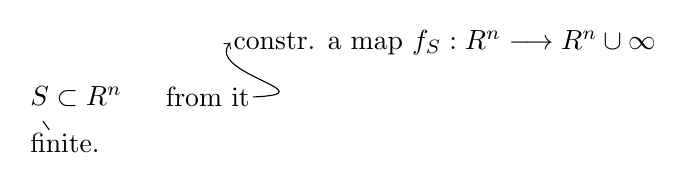
\begin{tikzpicture}[x=1cm,y=.85cm,every node/.style={inner sep=1pt,anchor=west}]
\node (map) at (2.58,.81) {constr. a map \(f_S:\mathbb R^n\longrightarrow\mathbb R^n\cup\infty\)};
\node at (0,0) {\(S\subset\mathbb R^n\)};
\node at (0,-.69) {finite.};
\node (by) at (1.72,0) {from it};
\draw[->] (by.east) .. controls +(1,.05) and +(-.32,-.46) .. (map.west);
\draw (0.20,-.36)--(.28,-.49);
\end{tikzpicture}}\endgroup
\par
\Unclear{GELFAND-P000569}{map-verb}{The abbreviation before “map” reads “стр.” An arrow points up to it.}
\end{GelfandAdjacentEvidence}
\begin{GelfandAdjacentEvidence}{GELFAND-P000569}{5}

\Unclear{GELFAND-P000569}{german-word}{The end of the word merges with the arrow. It provisionally reads “from it”, possibly “after the German”.}
\end{GelfandAdjacentEvidence}
\begin{GelfandAdjacentEvidence}{GELFAND-P000569}{6}

\(E\) — field strength (electr.), produced by unit charges at points \(x\in S\). We get a vector \(E\in\mathbb R^n\cup\infty\)
\SourceFigure{GELFAND-P000569}{charge-vector}{%
\par\smallskip
\begingroup\color{black}\GelfandFitDiagram{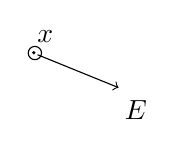
\begin{tikzpicture}[x=.77cm,y=.72cm,every node/.style={inner sep=1pt}]
\draw (0,0) circle (2.4pt);
\fill (-.018,.006) circle (.65pt);
\draw[->] (.045,-.03)--(1.38,-.61);
\node[above] at (.17,.13) {$x$};
\node[below right] at (1.43,-.78) {$E$};
\end{tikzpicture}}\endgroup\par}
\end{GelfandAdjacentEvidence}
\begin{GelfandAdjacentEvidence}{GELFAND-P000569}{7}

At the points \(x\in S\) it will be \(\infty\).
\hfill\uwave{\mbox{$\infty\longrightarrow0$}}\par
\[
f_S:\mathbb R^n\cup\infty\longrightarrow\mathbb R^n\cup\infty
\]
We get a map
\[
\begingroup\color{black}\GelfandFitDiagram{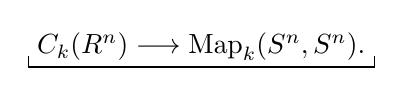
\begin{tikzpicture}[baseline=(mapping.base)]
\node[inner xsep=3pt,inner ysep=2pt] (mapping)
 {$C_k(\mathbb R^n)\longrightarrow\mathrm{Map}_k(S^n,S^n).$};
\draw ([yshift=4pt]mapping.south west) -- (mapping.south west) -- (mapping.south east)
      -- ([yshift=4pt]mapping.south east);
\end{tikzpicture}}\endgroup
\qquad(\text{\uwave{map of degree \mbox{$k$}}}).
\]
(When far away, all \(k\) points are perceived as one).
\Unclear{GELFAND-P000569}{far-overwrites}{The \(k\) and the end of the Russian word for “points” are written over. The earlier strokes are illegible.}
\end{GelfandAdjacentEvidence}
\begin{GelfandAdjacentEvidence}{GELFAND-P000569}{8}

A point corresp. to a long vector — near one of the \(k\) charges

— and there are such points.
\Unclear{GELFAND-P000569}{such-word}{A letter in the middle of the Russian word for “such” is heavily overwritten. The earlier strokes are illegible.}
\end{GelfandAdjacentEvidence}
\begin{GelfandAdjacentEvidence}{GELFAND-P000569}{9}

\(C_k(\mathbb R^n)\) — a good approx. of \(\mathrm{Map}_k(S^n,S^n)\)!! (in a certain sense)

A good approx. for large \(k\).
\[
H_i(C_k(\mathbb R^n))\underset{\cong}{\longrightarrow}H_i(\mathrm{Map}_k)
\]
\hfill for \(i\ll k\)\qquad (there are many proofs, including Segal’s)\par
\Unclear{GELFAND-P000569}{homology-arrow-lower-mark}{Below the arrow is a wave over two horizontal strokes, in the form \(\cong\).}
\end{GelfandAdjacentEvidence}
\begin{GelfandAdjacentEvidence}{GELFAND-P000569}{10}

\uwave{Inventiones}
\Unclear{GELFAND-P000569}{invection-word}{The underlined word reads “Inventiones”. The final letters are joined.}
\end{GelfandAdjacentEvidence}



\Needspace{7\baselineskip}
\begin{GelfandAdjacentEvidence}{GELFAND-P000570}{1}
\SourcePage{GELFAND-P000570}{unlabelled}
A generalization of this thm. will be described (due to \sout{[…]} Dusa Mc Duff)
\Incomplete{GELFAND-P000570}{attribution-old}{A short entry before the name “Dusa Mc Duff” is crossed out and illegible.}
\end{GelfandAdjacentEvidence}
\begin{GelfandAdjacentEvidence}{GELFAND-P000570}{2}

\noindent\hfill\rule{.66cm}{.32pt}\enspace\rule{.64cm}{.32pt}\par
\uuline{Fuchs.}\quad \(C_k(\mathbb R^n)\) gives various classifying spaces.
\Unclear{GELFAND-P000570}{fuchs-overwrite}{The initial letter of “Fuchs” is written over with a heavy stroke. The earlier strokes remain unresolved.}
\end{GelfandAdjacentEvidence}
\begin{GelfandAdjacentEvidence}{GELFAND-P000570}{3}

\noindent\hfill\rule{.72cm}{.32pt}\enspace\(\cdot\)\enspace\rule{.91cm}{.32pt}\par
\uwave{2 kinds of questions arise}:

The right side is indep. of \(k\) (\(\approx\)), on the left pass to the limit in \(k\).
\Unclear{GELFAND-P000570}{limit-overwrite}{The middle of the Russian word for “limit” is written over. The earlier strokes are illegible.}
\end{GelfandAdjacentEvidence}
\begin{GelfandAdjacentEvidence}{GELFAND-P000570}{4}

(homot. eq.)

\(C_k^\pm(\mathbb R^n)\qquad\) finite subsets with charges of diff. signs

topology — if 2 oppositely charged particles approach, they disappear.

Many components (total charge), \(-\infty<k<+\infty\)

Does not depend strongly on \(k\).
\[
C_k^\pm(\mathbb R^n)\underset{2}{\simeq}\mathrm{Map}_k(S^n,S^n)
\]
\Unclear{GELFAND-P000570}{signed-comparison}{A separate mark in the shape of \(2\) is below \(\simeq\). Its meaning remains unresolved.}
\end{GelfandAdjacentEvidence}
\begin{GelfandAdjacentEvidence}{GELFAND-P000570}{5}

\uwave{a very good approx.} (hypothesis). or
\Unclear{GELFAND-P000570}{hypothesis-old}{Heavy crossing strokes follow “hypothesis”. The provisional reading is “or”.}
\end{GelfandAdjacentEvidence}
\begin{GelfandAdjacentEvidence}{GELFAND-P000570}{6}

There is a space \(Y_n,\qquad\dim Y_n=2n\),
\[
\underline{C_k^\pm(\mathbb R^n)\simeq\mathrm{Map}_k(S^n,Y_n)}.
\]
\Unclear{GELFAND-P000570}{target-relation}{The upper stroke of the relation is written over. The visible wave over a line is transcribed as \(\simeq\).}
\end{GelfandAdjacentEvidence}
\begin{GelfandAdjacentEvidence}{GELFAND-P000570}{7}

\Unclear{GELFAND-P000570}{target-overwrite}{The \(Y\) in the final \(Y_n\) is written over. The earlier strokes are illegible.}
\end{GelfandAdjacentEvidence}
\begin{GelfandAdjacentEvidence}{GELFAND-P000570}{8}

\underline{\(C_k(M)\)}\qquad \underline{\(M\) — a manifold}

What in place of \(\mathrm{Map}(S^n,S^n)\)?
\[
C_k(M)\longrightarrow\Gamma(T_M^{\mathrm{comp}}),
\]
\uwave{\mbox{$\infty$} is added in each fibre}. (all fibres compactified).

At \sout{[…]} infinity one can take \(0\) (with comp. supp.)
\Unclear{GELFAND-P000570}{infinity-old}{A small loop-shaped mark is crossed out before “infinity”. Its reading remains unresolved.}
\end{GelfandAdjacentEvidence}
\begin{GelfandAdjacentEvidence}{GELFAND-P000570}{9}

\[
C_k(M)\longrightarrow\Gamma_k^{\mathrm{cpt}}(T_M^{\mathrm{comp}})
\]
induces a homol. isom. for \(i\ll k\).

(The electr. field is taken to have finite range — then everything is constr.)

\uline{The proof method is of greater interest than the assertion}.

\(U\subset M\)\quad a small piece of \(M\).
\qquad \(C_k(U)\)\ \sout{[…]}\ \(C_k(M)\).
\Unclear{GELFAND-P000570}{inclusion-old}{A sign between \(C_k(U)\) and \(C_k(M)\) is heavily crossed out. Its reading remains unresolved.}
\end{GelfandAdjacentEvidence}
\begin{GelfandAdjacentEvidence}{GELFAND-P000570}{10}

We would like to obtain \(C_k(M)\), by joining \(C_k(U)\).
\SourceFigure{GELFAND-P000570}{overlap-path}{%
\par\smallskip
\begingroup\color{black}\GelfandFitDiagram{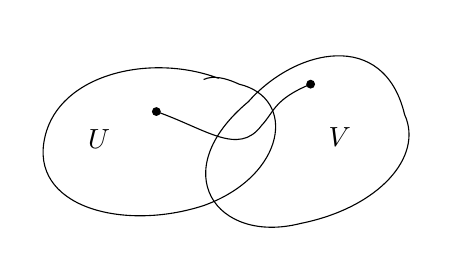
\begin{tikzpicture}[x=.79cm,y=.74cm,every node/.style={inner sep=1pt}]
\draw (1.35,1.12) .. controls (.25,1.56) and (-1.21,1.19) .. (-1.44,.12)
  .. controls (-1.71,-1.08) and (-.19,-1.52) .. (1.12,-1.06)
  .. controls (2.43,-.55) and (2.62,.78) .. (1.68,1.02)
  .. controls (1.48,1.12) and (1.27,1.18) .. (1.11,1.10);
\draw (4.34,.50) .. controls (4.01,1.98) and (2.58,1.63) .. (1.83,.72)
  .. controls (.48,-.48) and (1.31,-1.74) .. (2.67,-1.37)
  .. controls (3.93,-1.10) and (4.65,-.22) .. (4.34,.50);
\draw (.35,.55) .. controls (1.15,.25) and (1.67,-.22) .. (2.04,.31)
  .. controls (2.25,.55) and (2.24,.76) .. (2.83,1.02);
\fill (.35,.55) circle (1.6pt) (2.83,1.02) circle (1.6pt);
\node at (-.57,.08) {$U$};
\node at (3.30,.11) {$V$};
\end{tikzpicture}}\endgroup\par}
\end{GelfandAdjacentEvidence}
\begin{GelfandAdjacentEvidence}{GELFAND-P000570}{11}

\[
C(M)\underset{\text{discontinuous}}{\longrightarrow} C(U)\times C(V)
\]
\Unclear{GELFAND-P000570}{restriction-note}{“Discontinuous” is written below the formula and above the next line.}
\end{GelfandAdjacentEvidence}

Let \(U,V\) — manifolds with boundary.

\(\overline C(U)\) — the quotient space of \(C(U)\)
\[
S_1\sim S_2\quad\Leftrightarrow\quad S_1\cap\overset{\circ}U=S_2\cap\overset{\circ}U
\]
(points on the boundary disappear)

\underline{Thm.}\quad \(U\) — a manif. with boundary (nonempty)
\[
\Rightarrow\quad\overline C(U)\underset{\simeq}{\longrightarrow}
\Gamma(TU^{\mathrm{comp}})\qquad(\text{homotopic equiv.}).
\]
\underline{Proof.}\quad\uuline{Case~1.}\qquad \(U=\) the unit disk.

\uwave{Left side}: \(C_\varepsilon(U)\) — configurs. with distance \(>\varepsilon\).
Configurs. of \(\leqslant1\) \uwave{particles remain}.

right side\qquad \(\mathrm{Map}(U,S^n)\simeq S^n\)

Radial stretch. \(\longrightarrow S^n\) (pushed out to the boundary)


\Needspace{7\baselineskip}
\begin{GelfandAdjacentEvidence}{GELFAND-P000571}{1}
\SourcePage{GELFAND-P000571}{unlabelled}
\SourceFigure{GELFAND-P000571}{cover-circles}{%
\par\smallskip
\begingroup\color{black}\GelfandFitDiagram{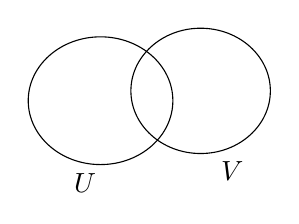
\begin{tikzpicture}[x=.82cm,y=.78cm,every node/.style={inner sep=1pt}]
\draw (0,0) ellipse (1.12 and 1.04);
\draw (1.55,.16) ellipse (1.08 and 1.02);
\node[below] at (-.24,-1.14) {$U$};
\node[below] at (2.04,-.94) {$V$};
\end{tikzpicture}}\endgroup\par}
\end{GelfandAdjacentEvidence}
\begin{GelfandAdjacentEvidence}{GELFAND-P000571}{2}

\SourceFigure{GELFAND-P000571}{cover-diagram}{%
\par\smallskip
\begingroup\color{black}\GelfandFitDiagram{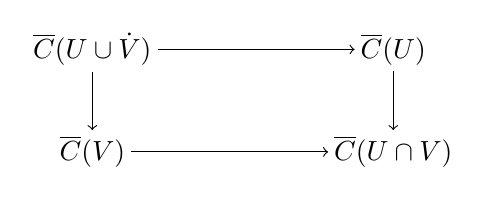
\begin{tikzpicture}[x=.84cm,y=.84cm,every node/.style={inner sep=2pt}]
\node (A) at (0,0) {$\overline C(U\cup\dot V)$};
\node (B) at (4.55,0) {$\overline C(U)$};
\node (C) at (0,-1.55) {$\overline C(V)$};
\node (D) at (4.55,-1.55) {$\overline C(U\cap V)$};
\draw[->] (A)--(B);
\draw[->] (A)--(C);
\draw[->] (B)--(D);
\draw[->] (C)--(D);
\end{tikzpicture}}\endgroup\par
A dot stands above \(V\) in the upper left. Its meaning remains unresolved. The lower arrow points right.}
\end{GelfandAdjacentEvidence}
\begin{GelfandAdjacentEvidence}{GELFAND-P000571}{3}

there are well-defined maps and if 2 points from \(\overline C(U)\) and \(\overline C(V)\) det. one in
\(\overline C(U\cap V)\), then \sout{this} det. a point in \(\overline C(U\cup V)\).
\Unclear{GELFAND-P000571}{cancelled-pronoun}{“This” is crossed out after “then”.}
\end{GelfandAdjacentEvidence}
\begin{GelfandAdjacentEvidence}{GELFAND-P000571}{4}

\SourceFigure{GELFAND-P000571}{section-square}{%
\par\smallskip
\begingroup\color{black}\GelfandFitDiagram{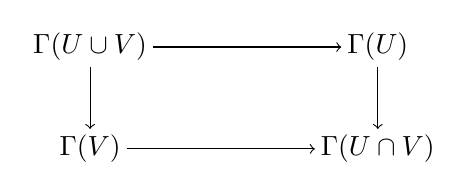
\begin{tikzpicture}[x=.84cm,y=.84cm,every node/.style={inner sep=2pt}]
\node (A) at (0,0) {$\Gamma(U\cup V)$};
\node (B) at (4.35,0) {$\Gamma(U)$};
\node (C) at (0,-1.54) {$\Gamma(V)$};
\node (D) at (4.35,-1.54) {$\Gamma(U\cap V)$};
\draw[->] (A)--(B);
\draw[->] (A)--(C);
\draw[->] (B)--(D);
\draw[->] (C)--(D);
\end{tikzpicture}}\endgroup\par}
\end{GelfandAdjacentEvidence}
\begin{GelfandAdjacentEvidence}{GELFAND-P000571}{5}

\uwave{Props. of covering homotopy}.
\Unclear{GELFAND-P000571}{homotopy-phrase}{The middle Russian abbreviation reads “накр.”.}
\end{GelfandAdjacentEvidence}

\noindent\hfill\rule{.95cm}{.32pt}\enspace\(\cdot\)\enspace\rule{1.05cm}{.32pt}\par
the analogous thm. on \(C_k(M)\) is omitted.

\noindent\hfill\rule{1.05cm}{.32pt}\enspace\(\cdot\)\enspace\rule{.89cm}{.32pt}\par
\underline{Next time}: Polyakov or Dubrovin.


\Needspace{7\baselineskip}
\begin{GelfandAdjacentEvidence}{GELFAND-P000572}{1}
\SourcePage{GELFAND-P000572}{unlabelled}
\underline{7/X--74.}\qquad\underline{Gelfand Sem.}

\underline{Kushnirenko.}\qquad \(f(z_1,\ldots,z_n)=\sum a_m z^m\)

\(0\) — sing. point. (series without const. and linear terms).

Milnor number \(\mu(f)\) \(=\) multiplicity of the zero sol.
\[
\frac{\partial f}{\partial z_1}=0,\ldots,\frac{\partial f}{\partial z_n}=0.
\]
\noindent\hfill\begin{minipage}{.47\linewidth}
\noindent\vrule width .35pt\hspace{1pt}\vrule width .35pt\enspace
\begin{minipage}{.88\linewidth}
— \underline{\(\max\)} \uwave{number} \sout{[\ldots]} \sout{[\ldots]} \uwave{sols.}\\
\(\dfrac{\partial f}{\partial z_i}=\varepsilon_i\)\\
\uwave{for small \(\varepsilon\)}.
\end{minipage}
\end{minipage}\par
\Incomplete{GELFAND-P000572}{margin-old}{Two groups in the right margin are crossed out after “number” and before “sols.”. Remnants of strokes are visible. The full reading remains unresolved.}
\end{GelfandAdjacentEvidence}
\begin{GelfandAdjacentEvidence}{GELFAND-P000572}{2}


Problem: compute \(\mu(f)\) from the coeffs. of the Taylor series.

\underline{2-dim. case.}\quad(\underline{\(n=2\)})
\SourceFigure{GELFAND-P000572}{newton-polygon}{%
\par\smallskip
\begingroup\color{black}\GelfandFitDiagram{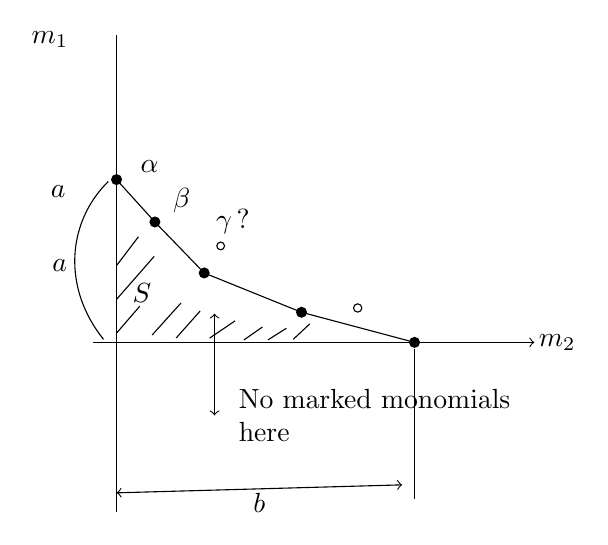
\begin{tikzpicture}[x=.87cm,y=.78cm,every node/.style={inner sep=1.4pt}]
\draw (0,-.16)--(0,5);
\draw[->] (-.35,0)--(6.1,0) node[right] {$m_2$};
\node[left] at (-.64,4.93) {$m_1$};
\draw (0,2.65)--(.56,1.96)--(1.28,1.13)--(2.7,.49)--(4.35,0);
\foreach \point in {(0,2.65),(.56,1.96),(1.28,1.13),(2.7,.49),(4.35,0)}
  \fill \point circle (2pt);
\draw (3.52,.56) circle (1.5pt);
\draw (1.52,1.57) circle (1.4pt);
\node[above] at (.48,2.7) {$\alpha$};
\node[above] at (.95,2.04) {$\beta$};
\node[above] at (1.7,1.69) {$\gamma\,?$};
\draw (-.19,.05) .. controls (-.79,.88) and (-.73,1.95) .. (-.12,2.62);
\node[left] at (-.66,1.25) {$a$};
\node[left] at (-.68,2.46) {$a$};
\draw (0,.15)--(.34,.59) (0,.7)--(.55,1.4) (0,1.25)--(.32,1.72)
      (.52,.12)--(.94,.64) (.87,.07)--(1.22,.51) (1.36,.07)--(1.73,.35)
      (1.86,.04)--(2.13,.25) (2.21,.04)--(2.48,.23) (2.58,.05)--(2.82,.3);
\node at (.37,.81) {$S$};
\draw (0,-.12)--(0,-2.76) (4.35,-.11)--(4.35,-2.55);
\draw[<->] (0,-2.45)--(4.17,-2.32) node[midway,below] {$b$};
\draw[<->] (1.43,-1.19)--(1.43,.47);
\node[anchor=west,align=left] at (1.72,-1.19) {No marked monomials\\here};
\end{tikzpicture}}\endgroup\par
The third label is written over. Its shape and the formula below suggest \(\gamma\). The reading remains provisional. The two small marks above the polygonal line are retained.}
\end{GelfandAdjacentEvidence}
\begin{GelfandAdjacentEvidence}{GELFAND-P000572}{3}

\uwave{conv. polygonal line}
\[
\nu(f)=2S-a-b+1.
\]
\uuline{Theorem}: \quad 1) \(\mu(f)\geqslant\nu(f)\)

2) \(\mu(f)=\nu(f)\), if certain nondegeneracy conds. hold

\(\beta^2\ne 4\alpha\gamma\) \quad
\((\alpha,\beta,\gamma\) — coefficients of the resp. monomials\()\).

(in the gen. case \(\ne0\) discriminant of the \uwave{left edge}.)

\hfill \(\searrow\) on the edge essentially a polynomial of 1 var.\par

\uuline{\(n=3.\)}
\[
\nu(f)=3!V-2!(S_{12}+S_{13}+S_{23})+1!(L_1+L_2+L_3)-1.
\]
\(S_{12}\) — area obtained on the plane.
\SourceFigure{GELFAND-P000572}{coordinate-section}{%
\par\smallskip
\begingroup\color{black}\GelfandFitDiagram{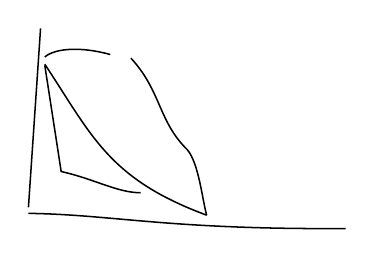
\begin{tikzpicture}[x=.77cm,y=.77cm,line width=.55pt]
\draw (0,.1)--(.2,3.05);
\draw (0,0).. controls (1.4,-.02) and (2.3,-.27) .. (5.23,-.25);
\draw (.27,2.58).. controls (.45,2.73) and (.88,2.75) .. (1.35,2.62);
\draw (1.69,2.56).. controls (2.19,2.02) and (2.14,1.52) .. (2.62,1.05)
      .. controls (2.81,.83) and (2.87,.21) .. (2.94,-.03);
\draw (.27,2.46).. controls (1.05,1.28) and (1.32,.57) .. (2.94,-.03);
\draw (.27,2.44)--(.54,.69).. controls (1.08,.57) and (1.47,.34) .. (1.85,.34);
\end{tikzpicture}}\endgroup\par
The contours and their spatial relation are schematic in the manuscript.}
\end{GelfandAdjacentEvidence}
\begin{GelfandAdjacentEvidence}{GELFAND-P000572}{4}

\Unclear{GELFAND-P000572}{section-detached-stroke}{A short detached oblique stroke is visible between the formula for \(\nu\) and the drawing. Its function is unresolved.}
\end{GelfandAdjacentEvidence}


\uuline{Theorem}: \quad 1) \(\mu(f)\geqslant\nu(f)\)

2) nondegen. cond. \(\Rightarrow\) \underline{equal-ty}.

\hspace{1.5em}(holds almost always)


\Needspace{7\baselineskip}
\begin{GelfandAdjacentEvidence}{GELFAND-P000573}{1}
\SourcePage{GELFAND-P000573}{unlabelled}
\SourceFigure{GELFAND-P000573}{face-cone}{%
\par\smallskip
\begingroup\color{black}\GelfandFitDiagram{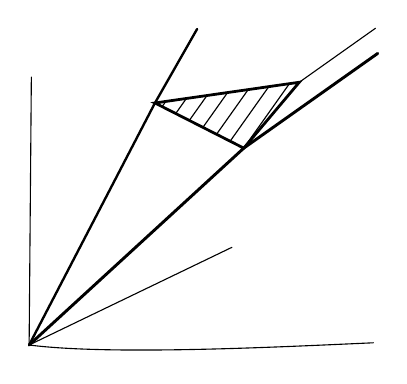
\begin{tikzpicture}[x=.94cm,y=.94cm,line cap=round]
\draw (.03,3.62)--(0,0).. controls (1.1,-.14) and (3.3,-.03) .. (4.65,.03);
\draw (0,0)--(2.74,1.32);
\draw[line width=.85pt] (0,0)--(1.7,3.27)--(2.27,4.27);
\draw[line width=1.05pt] (0,0)--(2.9,2.66)--(4.71,3.94);
\draw[line width=.4pt] (2.9,2.66)--(3.65,3.55)--(4.68,4.28);
\begin{scope}
\clip (1.7,3.27)--(3.65,3.55)--(2.9,2.66)--cycle;
\foreach \x in {1.30,1.55,1.80,2.05,2.30,2.55,2.80,3.05,3.30}
  \draw[line width=.42pt] (\x,2.52)--++(.9,1.27);
\end{scope}
\draw[line width=1pt] (1.7,3.27)--(3.65,3.55)--(2.9,2.66)--cycle;
\end{tikzpicture}}\endgroup\par
The hatched region lies between the upper rays. Heavy and retraced strokes are drawn schematically. The precise directions of the extensions are unresolved.}
\end{GelfandAdjacentEvidence}
\begin{GelfandAdjacentEvidence}{GELFAND-P000573}{2}

\[
z_i\frac{\partial f_\Delta}{\partial z_i}
\]
\uwave{\(f_\Delta\) — corresp. to the monomials of the face.}
\[
\dim_{\mathbb C}\mathbb C[P(\Delta)]\big/\left(z_i\frac{\partial f}{\partial z_i}\right)<\infty.
\]
\hfill nondegen. cond.\par

\underline{Proof}: commut. algebra. Use that \(\mathbb C[P(\Delta)]\) — a Cohen–Macaulay ring (Hochster).

\uuline{Arnold}.
\[
\sum_{\substack{x,y:\left\{\begin{smallmatrix}P_n(x,y)=0\\Q_n(x,y)=0\end{smallmatrix}\right.}}^{n^2}
\frac{R_{n-4}(x,y)}{\det\frac{\partial(P_n\,Q)}{\partial(x,y)}}=0.
\]
\Unclear{GELFAND-P000573}{jacobian-denominator}{The numerator of the Jacobian shows \(Q\) after \(P_n\). No distinct comma is visible, and any index on \(Q\) is obscured by the tail and parenthesis. The summation conditions separately show \(Q_n\).}
\end{GelfandAdjacentEvidence}
\begin{GelfandAdjacentEvidence}{GELFAND-P000573}{3}

\(P_n(x,y)\), \(Q_n(x,y)\) — 2 \uwave{polynomials}.

(\underline{\(R\) — an arb. polynomial} of deg. \(\le n-4\))

\hfill\uwave{\(\sum\) over all zeros}.\par

\uuline{Polyakov}. Consider \(\mathbb Z^2\) and a fn. of an oriented edge connecting adjacent vertices.
\SourceFigure{GELFAND-P000573}{yellow-mark}{A yellow icon with three strokes is visible above the word for “oriented” in the raster. Its text is absent from the image and its origin is unresolved.}
\end{GelfandAdjacentEvidence}
\begin{GelfandAdjacentEvidence}{GELFAND-P000573}{4}

\uwave{Yang–Mills fields}.
\[
B_{\tau,\alpha},\quad \tau\in\mathbb Z^2,\quad \alpha\text{ — dir.}
\]
a fn. with vals. in \(\mathrm{SU}(2)\) (or another compact gr.).
\SourceFigure{GELFAND-P000573}{edge-directions}{%
\par\smallskip
\begingroup\color{black}\GelfandFitDiagram{\begin{tikzpicture}[x=1cm,y=1cm]
\fill (0,0) circle (1.6pt);
\draw[->] (0,0)--(0,1.54) node[midway,left] {$\beta\,?$};
\draw[->] (0,0)--(1.76,.13) node[near end,below] {$\alpha$};
\node[below] at (0,0) {$\tau$};
\end{tikzpicture}}\endgroup\par
The label by the vertical arrow resembles \(\beta\), but its shape is ambiguous. The horizontal arrow is labelled \(\alpha\).}
\end{GelfandAdjacentEvidence}
\begin{GelfandAdjacentEvidence}{GELFAND-P000573}{5}

\[
F_{\vec\tau,\alpha\beta}
=\quad\begingroup\color{black}\GelfandFitDiagram{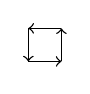
\begin{tikzpicture}[baseline=-.35ex,x=.42cm,y=.42cm,line width=.5pt]
\draw[->] (1,1)--(0,1);
\draw[->] (0,1)--(0,0);
\draw[->] (0,0)--(1,0);
\draw[->] (1,0)--(1,1);
\end{tikzpicture}}\endgroup
\quad\text{circul.}
=B_{\tau\alpha}B_{\tau+a_\alpha,\beta}B_{\tau+a_\beta,\alpha}^{-1}B_{\tau\beta}^{-1}.
\]
\SourceFigure{GELFAND-P000573}{plaquette}{The top, left, bottom and right arrows point left, down, right and up, respectively.}
\end{GelfandAdjacentEvidence}
\begin{GelfandAdjacentEvidence}{GELFAND-P000573}{6}

(field strength of \sout{[\ldots]} \(B\)). \(\hookleftarrow\) field
\Unclear{GELFAND-P000573}{field-word-old}{The earlier word before \(B\) is crossed out, provisionally “of the contour”. The inserted word “field” appears below with a connecting stroke.}
\end{GelfandAdjacentEvidence}
\begin{GelfandAdjacentEvidence}{GELFAND-P000573}{7}


Energy
\[
E=\sum_{\tau,\alpha,\beta}\chi(F_{\tau,\alpha,\beta})
\qquad
Z=\int\prod dB_{\tau,\alpha}\,e^{-\frac1T E[B]}.
\]
\Unclear{GELFAND-P000573}{energy-old}{A dense dark patch is visible above \(F\). The underlying sign and its function are unresolved.}
\end{GelfandAdjacentEvidence}
\begin{GelfandAdjacentEvidence}{GELFAND-P000573}{8}

\uwave{\(\chi\) — trace.}

Correl. fns.:
\[
\Pi(C)=Z^{-1}\int\prod dB_{\tau\alpha}\,\chi\left[\prod_{(C)}B_{\tau\lambda}\right]
   e^{-\frac1T E(B)}.
\]
\(\alpha,\beta=1\) or \(2\) \hfill \uwave{\(C\) — contour}.

Lattice of size \(N\times N\).

The planar prob. is solved exactly.
\begin{gather*}
\widetilde E=\sum_{\tau,\alpha}\chi(g_{\bar\tau}^{-1}g_{\vec\tau+\vec a_\alpha})\\
\widetilde{\widetilde E}
=\sum_{\tau,\alpha}\chi(g_{\bar\tau}^{-1}g_{\bar\tau+\bar a_\alpha} B_{\bar\tau,\alpha})
  \mathord{.}\,+E[B].
\end{gather*}
\Unclear{GELFAND-P000573}{double-tilde-energy}{In the double-tilde line \(B\) follows the second \(g\) within the parentheses with no visible comma between them. The \(\tau\) index on \(B\) has a bar. There is a small separate stroke near the baseline before the plus sign.}
\end{GelfandAdjacentEvidence}
\begin{GelfandAdjacentEvidence}{GELFAND-P000573}{9}


Field th. \(=\) stat. mech. in \(\mathbb R^n\) (Euclidean).

(Fourier transf. in time)

\underline{Sinai}.
\SourceFigure{GELFAND-P000573}{square-grid}{%
\par\smallskip
\begingroup\color{black}\GelfandFitDiagram{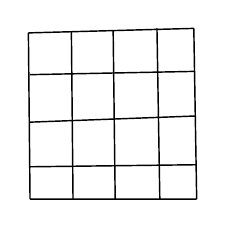
\begin{tikzpicture}[x=.52cm,y=.52cm,line width=.52pt]
\draw (0,0)--(-.04,4.06) (1.05,0)--(1.01,4.10) (2.08,0)--(2.03,4.12)
      (3.17,0)--(3.10,4.17) (4.07,0)--(4,4.17);
\draw (0,0)--(4.07,0) (0,.79)--(4.05,.84) (0,1.88)--(4.03,2.03)
      (0,3.04)--(4.02,3.12) (-.04,4.06)--(4,4.17);
\end{tikzpicture}}\endgroup\par}
\end{GelfandAdjacentEvidence}

\uwave{\(V\) — finite volume}.
\[
E(\{B_{\tau\alpha}\})=\sum\mathrm{tr}
\left(B_{\tau\alpha}B_{\tau+a_\alpha,\beta}B_{\tau+a_\beta,\alpha}^{-1}B_{\tau,\beta}^{-1}\right)
\]
\[
\underline{\underline{\mathcal M e^{-\beta E}=Z(\beta,V)}}
\]
Calculated for the 2-dim. case.
\[
\ln Z(\beta,V)=V\ln I_0(\beta)
\qquad (I_0(\beta)\text{ — Bessel fn.})
\]


\Needspace{7\baselineskip}
\begin{GelfandAdjacentEvidence}{GELFAND-P000574}{1}
\SourcePage{GELFAND-P000574}{unlabelled}
\[
B_{\tau\alpha}=e^{i A_{\tau\alpha}}
\]
\Unclear{GELFAND-P000574}{b-tight}{The first subscript on \(B\) and on \(A\) reads \(\tau\).}
\end{GelfandAdjacentEvidence}
\begin{GelfandAdjacentEvidence}{GELFAND-P000574}{2}


\[
\text{\sout{[\ldots]}}\ E=\sum\cos(A_{\tau\alpha}+A_{\tau+a_\alpha,\beta}-\ldots)
\]
\Unclear{GELFAND-P000574}{cancel-e-tight}{A short sign is densely crossed out before \(E\). \(\varphi\) is possible, but the reading is unresolved.}
\end{GelfandAdjacentEvidence}
\begin{GelfandAdjacentEvidence}{GELFAND-P000574}{3}

\Unclear{GELFAND-P000574}{e-index-tight}{The second \(A\) under the cosine has \(\tau+a_\alpha\), a comma and \(\beta\) in its subscript.}
\end{GelfandAdjacentEvidence}

\[
\lim_{V\to\infty}\frac{\ln Z(\beta,V)}{V}=f(\beta)
\]
\hfill\uwave{does not depend on the choice of boundary conds.}\par

\(f(\beta)\) may have singularities — they are called phase transitions.

(\(\approx\) a rearrangement of typical configs. occurs).

\[
p(\{B_{\tau,\alpha}\})=Z^{-1}e^{-\beta E(\{B_{\tau\alpha}\})}
\qquad\text{— Gibbs distrib.}
\]

Correl. fn. — mean value of the circulation around the contour.

\noindent
\begin{tabular}{@{}ll@{}}
Phase trans. — & in one phase \(\sim\) area\\
               & in the other \(\sim\) length.
\end{tabular}


\Needspace{7\baselineskip}
\begin{GelfandAdjacentEvidence}{GELFAND-P000575}{1}
\SourcePage{GELFAND-P000575}{unlabelled}
\sout{[\ldots]}\quad\underline{14/X--74.}\qquad\underline{Gelfand Sem.}
\Unclear{GELFAND-P000575}{cancel-date-tight}{A short group is crossed out before the date. The Russian letters “По” are possible, but the strokes overlap.}
\end{GelfandAdjacentEvidence}
\begin{GelfandAdjacentEvidence}{GELFAND-P000575}{2}


\uuline{Graeme Segal}.

\uuline{Classifying space of category.}

\(\mathcal C\) — category, \qquad \(|\mathcal C|\) is top. space

\uwave{Objects} — points

\uwave{Morphisms} — 1-dim symplex.

\uwave{Compositions — ?}
\SourceFigure{GELFAND-P000575}{graph-tight}{%
\par\smallskip
\begingroup\color{black}\GelfandFitDiagram{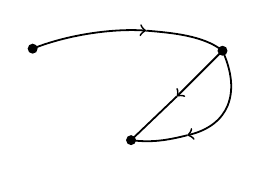
\begin{tikzpicture}[x=.88cm,y=.88cm,line width=.65pt]
\coordinate (A) at (0,1.32);
\coordinate (B) at (2.74,1.29);
\coordinate (C) at (1.42,0);
\draw[->] (A).. controls (.58,1.55) and (1.24,1.61) .. (1.64,1.58);
\draw (1.64,1.58).. controls (2,1.55) and (2.47,1.51) .. (B);
\draw[->] (B)--(2.08,.63);
\draw (2.08,.63)--(C);
\draw[->] (B).. controls (3.02,.67) and (2.82,.21) .. (2.23,.07);
\draw (2.23,.07).. controls (1.95,0) and (1.72,-.04) .. (C);
\foreach \v in {A,B,C} \fill (\v) circle (1.8pt);
\end{tikzpicture}}\endgroup\par}
\end{GelfandAdjacentEvidence}
\begin{GelfandAdjacentEvidence}{GELFAND-P000575}{3}

we have a \uwave{graph}.

It describe not cat. \([?]\)
\Unclear{GELFAND-P000575}{tail-loop}{A low loop-like sign follows “cat.”. The reading \(\mathcal C\) is tentative. Its shape differs from the clearly written letter above.}
\end{GelfandAdjacentEvidence}
\begin{GelfandAdjacentEvidence}{GELFAND-P000575}{4}

\hspace{1.1em}(composition!)
\SourceFigure{GELFAND-P000575}{compos-left}{%
\par\smallskip
\begingroup\color{black}\GelfandFitDiagram{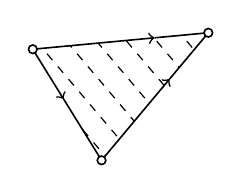
\begin{tikzpicture}[x=.91cm,y=.91cm,line width=.58pt]
\coordinate (A) at (0,1.55);
\coordinate (B) at (2.45,1.78);
\coordinate (C) at (.96,0);
\begin{scope}
\clip (A)--(B)--(C)--cycle;
\foreach \x in {-.5,-.1,.32,.74,1.16,1.58,2}
  \draw[dashed,line width=.43pt] (\x,1.84)--++(1.5,-1.77);
\end{scope}
\draw[->] (A)--(1.7,1.7096);
\draw (1.7,1.7096)--(B);
\draw[->] (A)--(.43,.8557);
\draw (.43,.8557)--(C);
\draw[->] (C)--(1.91,1.1349);
\draw (1.91,1.1349)--(B);
\foreach \v in {A,B,C} \filldraw[fill=white,draw=black] (\v) circle (1.55pt);
\end{tikzpicture}}\endgroup\par}
\end{GelfandAdjacentEvidence}
\begin{GelfandAdjacentEvidence}{GELFAND-P000575}{5}

\uwave{two-symplex} — \uwave{composition} of two morphisms.

\uwave{3 morph.}, and all compos. — \uwave{3-dim symplex}.

\hspace{2em}\fbox{\small which can be composed}\(\,\uparrow\)
\SourceFigure{GELFAND-P000575}{compos-right}{%
\par\smallskip
\begingroup\color{black}\GelfandFitDiagram{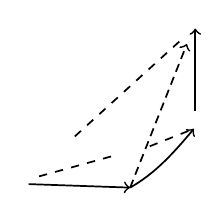
\begin{tikzpicture}[x=.89cm,y=.89cm,line width=.62pt]
\coordinate (A) at (0,0);
\coordinate (B) at (1.45,-.05);
\coordinate (C) at (2.36,.79);
\coordinate (D) at (2.38,2.22);
\draw[->] (A)--(B);
\draw[->] (B).. controls (1.8,.15) and (2.05,.42) .. (C);
\draw[->] (2.38,1.05)--(D);
\draw[->,densely dashed] (B)--(2.26,2);
\draw[dashed] (.15,.11)--(1.27,.42) (1.73,.54)--(C);
\draw[dashed] (.66,.68)--(2.18,2.06);
\end{tikzpicture}}\endgroup\par
The solid arrows and discernible thin strokes are drawn schematically. Some overlapping edges have unresolved directions.}
\end{GelfandAdjacentEvidence}
\begin{GelfandAdjacentEvidence}{GELFAND-P000575}{6}

etc.

We define \(|\mathcal C|\).

\underline{Diametr. opposed examples.}

\fbox{\small\uwave{Partially}}\(\,\downarrow\)

\uwave{Ordered sets}.

\(\equiv\) categ. with at most one morph. between two objects.

\underline{groups}
\SourceFigure{GELFAND-P000575}{group-tight}{%
\par\smallskip
\begingroup\color{black}\GelfandFitDiagram{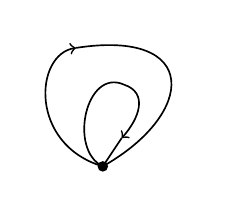
\begin{tikzpicture}[x=.85cm,y=.85cm,line width=.6pt]
\draw[->] (0,0).. controls (-1.11,.33) and (-1.02,1.68) .. (-.4,1.77);
\draw (-.4,1.77).. controls (1.46,2.06) and (1.4,.79) .. (0,0);
\draw[->] (0,0).. controls (-.52,.25) and (-.25,1.48) .. (.32,1.22)
  .. controls (.68,1.1) and (.55,.72) .. (.28,.42);
\draw (.28,.42)--(0,0);
\fill (0,0) circle (1.9pt);
\end{tikzpicture}}\endgroup\par
morphisms \(\cong\) \uwave{elts of group}\par
\uwave{one} object.\par
compos \(=\)\par
\(=\) comp. of elem.}
\end{GelfandAdjacentEvidence}


\noindent\rule{1.45cm}{.32pt}\enspace\(\cdot\)\enspace\rule{1.55cm}{.32pt}\par

\(X\) top space, \qquad \(\{U_\alpha\}_{\alpha\in S}\) — covering \qquad \(U_\alpha\subset X\)

\hspace{8em}\textit{open sets}

\underline{We suppose:}

\uwave{Property:}
\[
U_\alpha\cap U_\beta=\bigcup_{\text{certain }\gamma}U_\gamma.
\]
\[
\alpha\le\beta\quad\underset{\mathrm{def}}{\Longleftrightarrow}\quad U_\alpha\subset U_\beta.
\]
If all sets are contractible then
\(\lvert\mathcal C\rvert\underset{\text{hom. equiv.}}{\simeq}X\).

Add. intersections.


\Needspace{7\baselineskip}
\begin{GelfandAdjacentEvidence}{GELFAND-P000576}{1}
\SourcePage{GELFAND-P000576}{unlabelled}
\underline{Example.}\qquad \(X=S^2\). \hfill \(w=U\cap V\).
\SourceFigure{GELFAND-P000576}{sphere}{%
\par\smallskip
\begingroup\color{black}\GelfandFitDiagram{\begin{tikzpicture}[x=.89cm,y=.89cm,line width=.56pt]
\draw (0,0) ellipse (1.06 and .96);
\draw[dashed] (-1.06,.03).. controls (-.63,.37) and (.64,.36) .. (1.04,.03);
\draw[line width=.85pt] (-1.06,.03).. controls (-.75,-.49) and (.76,-.4) .. (1.04,.06);
\node[above right] at (.78,.72) {$U$};
\node[below] at (-.03,-1.1) {$V$};
\fill (-1.24,.45) circle (1.25pt);
\draw[line width=.32pt] (.05,.96)--(.16,.88);
\begin{scope}[xshift=3.25cm]
\draw (0,0) ellipse (1.12 and 1.22);
\begin{scope}[rotate=13]
\draw[line width=.68pt] (0,-.14) ellipse (1.12 and .46);
\draw[line width=.61pt] (0,-.14) ellipse (1.04 and .30);
\fill (-1.08,-.14) circle (1.2pt);
\draw (1.03,-.12) ellipse (.09 and .12);
\draw[line width=.34pt] (-.66,.15)--(-.48,.22) (.59,-.56)--(.78,-.50);
\end{scope}
\draw[line width=.35pt] (-1.04,.43).. controls (-1.11,.56) and (-.94,.92) .. (-.84,1);
\end{scope}
\end{tikzpicture}}\endgroup\par
A small mark is visible to the left of the upper outline. The band lines and side marks overlap in parts of the lower drawing.}
\end{GelfandAdjacentEvidence}
\begin{GelfandAdjacentEvidence}{GELFAND-P000576}{2}

\SourceFigure{GELFAND-P000576}{interval}{%
\par\smallskip
\begingroup\color{black}\GelfandFitDiagram{\begin{tikzpicture}[x=.85cm,y=.85cm,line width=.55pt]
\fill (0,1.5) circle (1.55pt) (1.3,1.57) circle (1.55pt) (2.6,1.5) circle (1.55pt);
\draw[->] (1.04,1.55)--(.24,1.50);
\draw[->] (1.55,1.56)--(2.36,1.5);
\node[anchor=west,inner sep=0pt] at (0,.82) {\small But \(W\) is not contractible.};
\node[left] at (0,0) {$\lvert\mathcal C\rvert=$};
\draw (0,0)--(2.6,0);
\foreach \x in {0,1.3,2.6} \filldraw[fill=white,draw=black] (\x,0) circle (1.48pt);
\node[right] at (2.83,0) {\small segment.};
\end{tikzpicture}}\endgroup\par}
\end{GelfandAdjacentEvidence}
\begin{GelfandAdjacentEvidence}{GELFAND-P000576}{3}

\[
\begin{aligned}
w&=W_1\cup W_2.\\
x_1&\in(W_1\cap W_2)_{\text{comp}}.\\
x_2&\in(W_1\cap W_2)_{\substack{\text{connected}\\\text{comp}}}.
\end{aligned}
\]
\Unclear{GELFAND-P000576}{conn-comp-placed}{“comp” is written to the right of the first parenthesis. “connected” with “comp” below follows the second.}
\end{GelfandAdjacentEvidence}
\begin{GelfandAdjacentEvidence}{GELFAND-P000576}{4}


\sout{oc?} — \uwave{surface of octahedron}.
\Unclear{GELFAND-P000576}{cancel-oc-tight}{Two loop-like letters are visible under the cancellation, tentatively “oc”.}
\end{GelfandAdjacentEvidence}
\begin{GelfandAdjacentEvidence}{GELFAND-P000576}{5}

\SourceFigure{GELFAND-P000576}{octa}{%
\par\smallskip
\begingroup\color{black}\GelfandFitDiagram{\begin{tikzpicture}[x=.96cm,y=.96cm,line cap=round]
\coordinate (A) at (0,1.12);
\coordinate (B) at (1.04,2.23);
\coordinate (C) at (1.73,2.49);
\coordinate (D) at (2.68,2.17);
\coordinate (E) at (1.82,1);
\coordinate (F) at (.43,0);
\draw[line width=.95pt] (A)--(B)--(C)--(D)--(E)--(F)--cycle;
\draw[line width=.9pt] (A)--(C)--(E)--(A);
\draw[line width=.43pt] (.75,1.68)--(.96,2.05) (1.02,1.48)--(1.12,1.85)
      (2.11,1.73)--(2.46,2.03) (1.29,.78)--(1.52,1.03)
      (.48,.2)--(.55,.72) (.48,.1)--(.72,.34);
\fill (A) circle (1.7pt);
\end{tikzpicture}}\endgroup\par
The redraw follows the clear outline and inner strokes. Some thin and superimposed edges are only partly discernible.}
\end{GelfandAdjacentEvidence}
\begin{GelfandAdjacentEvidence}{GELFAND-P000576}{6}


\noindent\hfill\rule{1.18cm}{.32pt}\enspace\(\cdot\)\enspace\rule{1.22cm}{.32pt}\par

\underline{Ex. 2}

\(V\) — finite dimensional vect. space (\(\forall\) field).

\(\mathcal C\) — cat of proper subspaces and inclusions.

\(\lvert\mathcal C\rvert=\) “building” of \(V\)
\hfill\uwave{building}

\hspace{5em}“immeuble”

\underline{Thm.} (Solomon — Tits).

\sout{[\ldots]}\quad \(\lvert\mathcal C\rvert\simeq\)
\(\underset{\text{(bouquet)}}{\text{wedge}}\)
of spheres of dim \((n-2)\)

\hfill\((n=\dim V)\),
\Unclear{GELFAND-P000576}{cancel-wedge-tight}{A cancelled group with a vertical and loops precedes \(\lvert\mathcal C\rvert\). An earlier \(\lvert\mathcal C\rvert\) is possible.}
\end{GelfandAdjacentEvidence}
\begin{GelfandAdjacentEvidence}{GELFAND-P000576}{7}


(quantity of spheres depends on field — infinite if the field is infinite).

\underline{Proof.}

1. If ord. set has max elt then \(\lvert\mathcal C\rvert\) is contractible.
\SourceFigure{GELFAND-P000576}{cone-proof}{%
\par\smallskip
\begingroup\color{black}\GelfandFitDiagram{\begin{tikzpicture}[x=.9cm,y=.9cm,line width=.55pt]
\coordinate (M) at (1.27,1.6);
\draw (0,0).. controls (.27,-.09) and (.71,-.09) .. (.96,.01);
\foreach \x in {0,.34,.64,.96,1.12} \draw (\x,0)--(M);
\draw (.4,.81)--(M);
\fill (M) circle (1.8pt);
\end{tikzpicture}}\endgroup\par
\uwave{evidente}.}
\end{GelfandAdjacentEvidence}
\begin{GelfandAdjacentEvidence}{GELFAND-P000576}{8}


max elements are \sout{[\ldots]} subsp. of codimension 1.
\Unclear{GELFAND-P000576}{cancel-subsp-tight}{A short abbreviation, possibly “vect”, is crossed out before “subsp.”.}
\end{GelfandAdjacentEvidence}
\begin{GelfandAdjacentEvidence}{GELFAND-P000576}{9}

\Incomplete{GELFAND-P000576}{cancel-subsp-loss}{Multiple horizontal strokes conceal the middle of the cancelled abbreviation.}
\end{GelfandAdjacentEvidence}
\begin{GelfandAdjacentEvidence}{GELFAND-P000576}{10}

\[
\lvert\mathcal C\rvert=\bigcup_{H\text{—hyperplanes}}\lvert\mathcal C_H\rvert.
\]
\(\mathcal C_H\) — is the cat of subspace \(W\),
\(0\underset{\text{strict}}{\subset}W\subseteq H\).
\Unclear{GELFAND-P000576}{subspace-order}{The manuscript uses inclusion signs: \(\subset\) annotated “strict” and \(\subseteq\) with a lower bar.}
\end{GelfandAdjacentEvidence}
\begin{GelfandAdjacentEvidence}{GELFAND-P000576}{11}


\(\lvert\mathcal C_H\rvert\) is contractible.

\hspace{3em}\underline{be given}\(\,\swarrow\)\par
Let \sout{[\ldots]} fixed \sout{hyperplane} line \(L\).
\Unclear{GELFAND-P000576}{fixed-tight-a}{A group between “Let” and “fixed” is crossed out, possibly “We”.}
\end{GelfandAdjacentEvidence}
\begin{GelfandAdjacentEvidence}{GELFAND-P000576}{12}

\Incomplete{GELFAND-P000576}{fixed-word-loss}{Dense slanted strokes obscure the full group. “be given” is written separately above the line.}
\end{GelfandAdjacentEvidence}
\begin{GelfandAdjacentEvidence}{GELFAND-P000576}{13}

\[
\text{Let}\quad Y=\bigcup_{H\supset L}\lvert\mathcal C_H\rvert\subset\lvert\mathcal C\rvert.
\]
\sout{[\ldots] \(\Rightarrow \dim(W\cap H_0)>0\) [\ldots]}
\Unclear{GELFAND-P000576}{cancel-formula}{The end of the cancelled line reads \(\dim(W\cap H_0)>0\). The sign before “dim” resembles an implication arrow, and the final stroke may be Cyrillic “и”.}
\end{GelfandAdjacentEvidence}
\begin{GelfandAdjacentEvidence}{GELFAND-P000576}{14}

\Incomplete{GELFAND-P000576}{cancel-formula-loss}{The opening and intervening parts of the cancelled line remain unresolved.}
\end{GelfandAdjacentEvidence}


\uwave{\(Y\) is contractible} because
\[
\underset{\text{contr.,}}{\lvert\mathcal C_{H_1}\rvert}\cap
\underset{\text{contr.}}{\lvert\mathcal C_{H_2}\rvert}
=\underset{\text{also contractible}}{\lvert\mathcal C_{H_1\cap H_2}\rvert}.
\]


\Needspace{7\baselineskip}
\begin{GelfandAdjacentEvidence}{GELFAND-P000577}{1}
\SourcePage{GELFAND-P000577}{unlabelled}
If \(Y\) is covered by pieces \(Y_i\) such that all
\(Y_{i_1}\cap\ldots\cap Y_{i_k}\)

is contractible (and not \sout{[\ldots]}
\(\overset{\text{vide}}{\text{\sout{empty?}}}\) \([?]\))
\(\Rightarrow Y\) contractible.
\Unclear{GELFAND-P000577}{vide-placed}{“vide” is above the crossed-out word, tentatively Russian “пусто”. A loop-like sign with a descender is to the right. Its reading is unresolved.}
\end{GelfandAdjacentEvidence}
\begin{GelfandAdjacentEvidence}{GELFAND-P000577}{2}

\Incomplete{GELFAND-P000577}{condition-word-loss}{The first short word after “not” is crossed out. “et” is possible, but the full lettering is indistinct.}
\end{GelfandAdjacentEvidence}
\begin{GelfandAdjacentEvidence}{GELFAND-P000577}{3}

\hspace{2em}\sout{[\ldots]}\par
\Unclear{GELFAND-P000577}{small-cancel}{The short cancellation below “is” begins with strokes that resemble “te”.}
\end{GelfandAdjacentEvidence}
\begin{GelfandAdjacentEvidence}{GELFAND-P000577}{4}

\Incomplete{GELFAND-P000577}{small-word-loss}{Dense crossing strokes obscure the ending.}
\end{GelfandAdjacentEvidence}
\begin{GelfandAdjacentEvidence}{GELFAND-P000577}{5}

\hfill in partial.\par
\[
\lvert\mathcal C\rvert=Y\cup\bigcup_{H\not\supset L}\lvert\mathcal C_H\rvert.
\]
\Unclear{GELFAND-P000577}{top-union-sign}{The union is indexed by \(H\not\supset L\). The negated curved sign has no separate lower bar.}
\end{GelfandAdjacentEvidence}
\begin{GelfandAdjacentEvidence}{GELFAND-P000577}{6}

\underline{Lemma 1.}

If \(X=Y\cup Y_1\cup\ldots\cup Y_k\)

and \(Y_{\text{\sout{?}}}\), \(Y_1,\ldots,Y_k\) contractible.
\Unclear{GELFAND-P000577}{lemma-cancel}{A subscript on the first \(Y\) is crossed out. Its reading is unresolved.}
\end{GelfandAdjacentEvidence}
\begin{GelfandAdjacentEvidence}{GELFAND-P000577}{7}

and \(Y_i\cap Y_j\subset Y\), then
\[
X\simeq\underset{\text{\uwave{wedge}}}{\bigvee}\,
Y_i/(Y_i\cap Y)
\]
\Unclear{GELFAND-P000577}{lemma-math}{The numerator resembles \(Y_i\). The short stroke at its foot matches \(Y\) in the denominator. \(V_i\) remains a possible reading.}
\end{GelfandAdjacentEvidence}
\begin{GelfandAdjacentEvidence}{GELFAND-P000577}{8}

\SourceFigure{GELFAND-P000577}{collapse}{%
\par\smallskip
\begingroup\color{black}\GelfandFitDiagram{\begin{tikzpicture}[x=.77cm,y=.77cm,line width=.55pt]
\draw (-.75,-.95).. controls (-1.62,-.81) and (-1.05,.63) .. (-.44,1.13)
  .. controls (.5,1.75) and (1.3,1.11) .. (1.11,.37)
  .. controls (.83,-.58) and (.1,-.94) .. (-.75,-.95);
\draw (.83,1.13).. controls (1.4,1.57) and (2.34,1.26) .. (2.24,1.03)
  .. controls (2,.49) and (1.31,.12) .. (.63,.15);
\draw (.59,.33).. controls (1.36,.02) and (1.96,-.58) .. (1.8,-.79)
  .. controls (1.62,-1.01) and (.41,-.83) .. (.17,-.42);
\draw (-.54,-.46).. controls (-.92,-.75) and (-.98,-1.75) .. (-.47,-1.66)
  .. controls (.11,-1.64) and (.39,-.91) .. (.24,-.47);
\node at (-.47,.28) {$Y$};
\node at (2.35,1.46) {$Y_1$};
\node at (2.09,-.62) {$Y_2$};
\node at (.23,-1.71) {$Y_3$};
\fill (-.91,.68) circle (1.2pt);
\draw[dashed,->] (2.75,.8)--(4.46,.71);
\begin{scope}[xshift=4.16cm,yshift=.48cm]
\draw (0,0).. controls (.78,.93) and (1.58,.39) .. (1.05,.14)
  .. controls (.76,.01) and (.42,.09) .. (0,0);
\draw (0,0).. controls (-.66,.17) and (-1,-.56) .. (-.78,-.73)
  .. controls (-.5,-.9) and (-.21,-.54) .. (0,0);
\draw (0,0).. controls (.45,.15) and (.88,-.62) .. (.51,-.86)
  .. controls (.07,-.94) and (-.22,-.38) .. (0,0);
\fill (0,0) circle (1.6pt);
\end{scope}
\end{tikzpicture}}\endgroup\par
\(Y\) \uwave{collaps to point}}
\end{GelfandAdjacentEvidence}
\begin{GelfandAdjacentEvidence}{GELFAND-P000577}{9}


\underline{Lemma 2.}

Also if \(Z\) is contractible and \(Z_0\subset Z\) then
\[
Z/Z_0\simeq\underset{\text{suspension}}{SZ_0}
\]
\SourceFigure{GELFAND-P000577}{suspension}{%
\par\smallskip
\begingroup\color{black}\GelfandFitDiagram{\begin{tikzpicture}[x=.67cm,y=.67cm,line width=.54pt]
\begin{scope}[xshift=4.05cm,yshift=1.4cm]
\draw (-.58,0)--(0,.69)--(.58,.03)--(-.06,-.57)--cycle;
\draw (-.58,0)--(.58,.03);
\draw (-.28,.03)--(0,.69) (-.08,.03)--(0,.69) (.24,.03)--(0,.69);
\draw (-.22,-.07)--(-.17,-.39) (.02,-.08)--(-.01,-.36) (.2,-.09)--(.07,-.42);
\end{scope}
\draw[rotate=14] (0,0) ellipse (.9 and 1.12);
\draw[rotate=-24] (0,-.40) ellipse (.31 and .4);
\node at (-.2,.48) {$Z$};
\node at (0,-.37) {$Z_0$};
\begin{scope}[xshift=2cm]
\draw (-.55,-.34)--(0,.56)--(.55,-.32);
\draw (-.55,-.34).. controls (-.34,-.46) and (.33,-.48) .. (.55,-.32);
\draw (-.38,-.31)--(0,.56)--(.15,-.36) (.01,-.36)--(0,.56);
\draw[dashed] (-.54,-.31).. controls (-.26,-.13) and (.33,-.15) .. (.54,-.32);
\node[right] at (.65,.42) {$CZ_0$};
\node[below] at (0,-.5) {$Z_0$};
\end{scope}
\begin{scope}[xshift=4.05cm]
\draw (-.58,-.02)--(-.07,.63)--(.65,.06)--(-.17,-.58)--cycle;
\draw (-.58,-.02)--(.65,.06);
\draw (-.42,-.02)--(-.07,.63) (-.20,0)--(-.07,.63) (.18,.01)--(-.07,.63);
\draw (-.31,-.04)--(-.17,-.58) (-.04,-.04)--(-.17,-.58) (.25,-.02)--(-.17,-.58);
\node[right] at (.72,-.26) {$SZ_0$};
\end{scope}
\end{tikzpicture}}\endgroup\par}
\end{GelfandAdjacentEvidence}
\begin{GelfandAdjacentEvidence}{GELFAND-P000577}{10}

\[
\Rightarrow X\simeq\bigvee S(Y_i\cap Y)
\]

\underline{Lemma 3.}

\(\lvert\mathcal C_H\rvert\cap Y=\) “building” of \(H\).

and reduction by dimension.

\(\underline{\underline{\dim=2.}}\) (first step of induction).
\SourceFigure{GELFAND-P000577}{points-row}{%
\par\smallskip
\begingroup\color{black}\GelfandFitDiagram{\begin{tikzpicture}[x=.72cm,y=.72cm]
\fill (0,0) circle (1.2pt) (1.19,.025) circle (1.15pt) (2.17,-.01) circle (1.23pt);
\draw (3.37,-.035) ellipse (1.37pt and .91pt);
\draw (4.52,-.027) ellipse (1.22pt and .85pt);
\draw (5.52,-.02) ellipse (1.24pt and .85pt);
\fill (6.36,-.02) circle (1.18pt);
\end{tikzpicture}}\endgroup\par
Lines}
\end{GelfandAdjacentEvidence}
\begin{GelfandAdjacentEvidence}{GELFAND-P000577}{11}

wedge \fbox{\small of}!! points \sout{[\ldots]}
\Unclear{GELFAND-P000577}{lines-tight}{“of” is visible in an outline after “wedge”, with two vertical marks nearby. Their function is uncertain.}
\end{GelfandAdjacentEvidence}
\begin{GelfandAdjacentEvidence}{GELFAND-P000577}{12}

\sout{[\ldots]}
\Unclear{GELFAND-P000577}{lines-lower-tight}{Some strokes in the lower cancelled group resemble “wedge”.}
\end{GelfandAdjacentEvidence}
\begin{GelfandAdjacentEvidence}{GELFAND-P000577}{13}

\Incomplete{GELFAND-P000577}{lines-word-loss}{The lower inscription and the cancelled group after “points” are incompletely legible.}
\end{GelfandAdjacentEvidence}
\begin{GelfandAdjacentEvidence}{GELFAND-P000577}{14}


Suspension of wedge of spheres is also a wedge of spheres.

\(H_{n-2}(\lvert\mathcal C\rvert;\mathbb Z)=\) Steinberg module of \(V\).
\Unclear{GELFAND-P000577}{steinberg-relation}{Typeset as \(=\). The lower stroke is retraced, so \(\equiv\) is a possible reading.}
\end{GelfandAdjacentEvidence}
\begin{GelfandAdjacentEvidence}{GELFAND-P000577}{15}

(repres. in subgrps. of a fin. group)

\underline{Other extreme case.}

\(\mathcal C\) of group \(G\).\qquad
\(\lvert\mathcal C\rvert=BG\) — classifying space of group

\(\pi_1(\lvert\mathcal C\rvert)=G\). \qquad (\uwave{evidently})
\SourceFigure{GELFAND-P000577}{group-disc}{%
\par\smallskip
\begingroup\color{black}\GelfandFitDiagram{\begin{tikzpicture}[x=.92cm,y=.92cm,line width=.59pt]
\draw (0,0).. controls (.46,.83) and (1.01,2.05) .. (1.74,1.96)
  .. controls (2.72,1.8) and (2.68,.45) .. (1.91,-.26)
  .. controls (1.32,-.84) and (.66,-.68) .. (.12,-.31)
  .. controls (-.02,-.17) and (-.05,-.04) .. (0,0);
\draw (0,0).. controls (.7,.45) and (.77,1.49) .. (1.22,1.38)
  .. controls (1.79,1.29) and (1.35,.36) .. (.58,.16);
\draw[->] (1,.46).. controls (.88,.32) and (.74,.23) .. (.58,.16);
\draw (.58,.16).. controls (.36,.1) and (.15,.04) .. (0,0);
\draw (0,0).. controls (.47,.17) and (1.36,.27) .. (1.45,-.09)
  .. controls (1.46,-.73) and (.67,-.56) .. (.26,-.23);
\draw[->] (.69,-.47).. controls (.48,-.4) and (.35,-.3) .. (.26,-.23);
\draw (.26,-.23)--(0,0);
\draw[line width=.39pt] (1.2,1.09)--(1.82,1.65) (1.52,.79)--(2.09,1.28)
 (1.49,.47)--(2.16,.9) (1.58,.13)--(2.04,.45) (1.28,-.39)--(1.81,-.17);
\node at (1.54,.99) {$g_1$};
\node at (.98,-.23) {$g_2$};
\node[right] at (2.35,.16) {$g_1g_2$};
\end{tikzpicture}}\endgroup\par
The outline and loops follow the discernible strokes. Short, superimposed marks near the outline do not establish further directions.}
\end{GelfandAdjacentEvidence}


Universal covering is contractible.

Let \(\widetilde{\mathcal C}\) \qquad objects \(=\) elts of \(G\).

\(\exists\,1\) morph. \(g\to g'\) for each pair of elts.


\Needspace{7\baselineskip}
\begin{GelfandAdjacentEvidence}{GELFAND-P000578}{1}
\SourcePage{GELFAND-P000578}{unlabelled}
\(\lvert\widetilde{\mathcal C}\rvert\) is contractible.

(\(\forall\) el-t is connected by line with unity \(1\)).

\[
\widetilde{\mathcal C}\xrightarrow{\text{functor}}\mathcal C
\qquad\text{\uwave{universal covering space.}}
\]
\[
\begin{gathered}
g\mapsto *\\
\text{\uwave{\mbox{\(\tikz[baseline=(pair.base)]{\node[draw,ellipse,inner sep=1.7pt](pair){\(g\to g'\)};}
\mapsto g^{-1}g'\)}}}
\end{gathered}
\]
\SourceFigure{GELFAND-P000578}{chain-right}{%
\par\smallskip
\begingroup\color{black}\GelfandFitDiagram{\begin{tikzpicture}[x=.78cm,y=.78cm,line width=.53pt]
\node at (0,0) {$*$};
\node at (2,0) {$*$};
\node at (4,0) {$*$};
\node at (7.5,0) {$*$};
\draw[->] (.4,0)--(1.65,0) node[midway,above] {$g_1$};
\draw[->] (2.35,0)--(3.65,0) node[midway,above] {$g_2$};
\draw[->] (4.38,0)--(5.32,0);
\node at (5.73,0) {$\ldots$};
\draw[->] (6.35,0)--(7.12,0) node[midway,above] {$g_k$};
\draw[dashed] (0,-.2)--(0,-1.54);
\node[left] at (.02,-1.66) {$g$};
\draw[<-] (.08,-1.7)--(.98,-1.7);
\draw (1.04,-1.7) circle (.06);
\node at (1.77,-1.84) {$gg_1$};
\draw (2.85,-1.72)--(3,-1.72);
\draw[densely dotted] (4.07,-1.67) .. controls (4.8,-1.72) and (5.53,-1.75) .. (6.05,-1.64);
\draw[->] (6.36,-1.62)--(6.96,-1.62) node[midway,above] {$g_k$};
\node at (7.28,-1.7) {$*$};
\end{tikzpicture}}\endgroup\par
The short lower-left arrow points from a small loop towards \(g\). An asterisk is visible at the right.}
\end{GelfandAdjacentEvidence}
\begin{GelfandAdjacentEvidence}{GELFAND-P000578}{2}


\(\lvert\widetilde{\mathcal C}\rvert\to\lvert\mathcal C\rvert\)
\quad\uwave{universal covering.}
\[
\rule{1.8em}{.4pt}\;\boldsymbol{\cdot}\;\rule{1.8em}{.4pt}
\]
\SourceFigure{GELFAND-P000578}{bundle-diagram}{%
\par\smallskip
\begingroup\color{black}\GelfandFitDiagram{\begin{tikzpicture}[x=.84cm,y=.84cm,line width=.53pt]
\node (E) at (0,1.6) {$E$};
\node (X) at (0,0) {$X$};
\node (BG) at (3.25,0) {$BG$};
\draw[->] (E)--(X);
\draw[->] (X)--(BG) node[midway,below] {\uwave{classif. map}};
\node[right] at (.15,.94) {-- \sout{fibre space?}\enspace\uwave{bundle}};
\end{tikzpicture}}\endgroup\par}
\end{GelfandAdjacentEvidence}
\begin{GelfandAdjacentEvidence}{GELFAND-P000578}{3}

\Unclear{GELFAND-P000578}{bundle-tight}{The crossed-out expression next to “bundle” tentatively reads “fibre space”.}
\end{GelfandAdjacentEvidence}
\begin{GelfandAdjacentEvidence}{GELFAND-P000578}{4}


\(\{U_\alpha\}\) — covering, on \(U_\alpha\) bundle is trivial.
\Unclear{GELFAND-P000578}{covering-word}{A heavy superimposed stroke follows “covering” before the comma. A separate character is uncertain.}
\end{GelfandAdjacentEvidence}
\begin{GelfandAdjacentEvidence}{GELFAND-P000578}{5}

\SourceFigure{GELFAND-P000578}{inclusions}{%
\par\smallskip
\begingroup\color{black}\GelfandFitDiagram{\begin{tikzpicture}[x=.77cm,y=.77cm,line width=.52pt,font=\small]
\node (B) at (0,0) {$U_\beta$};
\node (I) at (2.04,0) {$U_\alpha\cap U_\beta$};
\node (A) at (4.13,0) {$U_\alpha$};
\draw[->] (I)--(B);
\draw[->] (I)--(A);
\draw[->] (1.28,-.92)--(.46,-.92) node[midway,below] {$g_{\beta,\alpha\beta}$};
\draw[->] (2.87,-.92)--(3.69,-.92) node[midway,below] {$g_{\alpha,\alpha\beta}$};
\node[right] at (3.9,-1.27) {$\in G$};
\node[right] at (4.35,-.77) {two immersions};
\end{tikzpicture}}\endgroup\par}
\end{GelfandAdjacentEvidence}
\begin{GelfandAdjacentEvidence}{GELFAND-P000578}{6}

Let us consider categ. of sets \(U_\alpha\) and their finite intersections

\sout{let \textellipsis{} this cat. of sets}
\Unclear{GELFAND-P000578}{cancel-line}{The crossed-out line shows “let”, tentatively “this”, and “cat. of sets”.}
\end{GelfandAdjacentEvidence}
\begin{GelfandAdjacentEvidence}{GELFAND-P000578}{7}

\Incomplete{GELFAND-P000578}{cancel-line-loss}{The strokes after “let” may include “us”. The full passage is indistinct.}
\end{GelfandAdjacentEvidence}

\[
\rule{1.8em}{.4pt}\;\boldsymbol{\cdot}\;\rule{1.8em}{.4pt}
\]


\Needspace{7\baselineskip}
\begin{GelfandAdjacentEvidence}{GELFAND-P000579}{1}
\SourcePage{GELFAND-P000579}{unlabelled}
\underline{21/\(\overline{\underline{\mathrm X}}\)-74.}
\quad \underline{Gelfand Sem.}\quad \underline{Kushnirenko.}

\uwave{Melvin Hochster.}

\(P\colon\mathbb C^n\to\mathbb C\), \(P\) — a polynomial,
\(P=\sum a_m z^m\).

Singular points: \(\{z:\frac{\partial P}{\partial z_i}=0\}\).
Consider all the sing. points. Suppose they are isolated.

How do we find them, counting multiplicity?

Consider the convex hull of \(0\) and all \(m\in\mathbb Z^n\) for which \(a_m\ne0\).
\SourceFigure{GELFAND-P000579}{polygon}{%
\par\smallskip
\begingroup\color{black}\GelfandFitDiagram{\begin{tikzpicture}[x=.67cm,y=.52cm,font=\small,line width=.46pt]
\foreach \i in {1,2,3,4} {
  \draw (\i,0)--(\i,4.05);
  \draw (0,\i)--(4.55,\i);
}
\draw[->] (0,0)--(5.45,0) node[right] {$m_1$};
\draw[->] (0,0)--(0,5.05) node[above right] {$m_2$};
\draw[line width=1.05pt] (0,0)--(0,2)--(1,4)--(4,2)--(2,0)--cycle;
\foreach \point in {(0,0),(0,2),(1,4),(4,2),(2,0)}
  \fill \point circle (2.05pt);
\node[left] at (0,1) {$a$};
\node[below] at (1,0) {$b$};
\end{tikzpicture}}\endgroup\par}
\end{GelfandAdjacentEvidence}
\begin{GelfandAdjacentEvidence}{GELFAND-P000579}{2}

\[
2S-a-b+1.
\]
1) the number of isol. sing. points, counting mult., \(\le 2S-a-b+1\).

2) if the nondegeneracy cond. holds \(=2S-a-b+1\).

\underline{Idea:} consider the degree of the map \(S^{2n-1}\to S^{2n-1}\).
\[
\overset{\lvert z\rvert=R}{z}
\longmapsto
\frac{\left(\frac{\partial P}{\partial z_1},\ldots,\frac{\partial P}{\partial z_n}\right)}
{\lvert\operatorname{grad}P\rvert}.
\]
This was known in the homogeneous or quasihomog. case.

\(\sum\) \uwave{of Milnor numbers} \(=\) \uwave{degree} \quad (abs. fact)
\SourceFigure{GELFAND-P000579}{degree-triangle}{%
\par\smallskip
\begingroup\color{black}\GelfandFitDiagram{\begin{tikzpicture}[x=.72cm,y=.72cm,line width=.53pt]
\draw (0,1.65)--(0,0)--(2.14,0);
\draw[line width=.87pt] (0,1.1)--(1.23,0);
\fill (0,0) circle (1.55pt) (0,1.1) circle (1.95pt) (1.23,0) circle (1.95pt);
\node[left] at (-.14,1.18) {$d$};
\node[below right] at (1.23,0) {$d$};
\end{tikzpicture}}\endgroup\par}
\end{GelfandAdjacentEvidence}
\begin{GelfandAdjacentEvidence}{GELFAND-P000579}{3}


\underline{Hochster:} consider the ring of monomials with exponents \(\underline{\underline m}\) in the angle.
\Unclear{GELFAND-P000579}{hochster}{The handwritten Russian preposition “в” before “угле” is retraced.}
\end{GelfandAdjacentEvidence}
\begin{GelfandAdjacentEvidence}{GELFAND-P000579}{4}

\SourceFigure{GELFAND-P000579}{hochster-cone}{%
\par\smallskip
\begingroup\color{black}\GelfandFitDiagram{\begin{tikzpicture}[x=.76cm,y=.76cm,line width=.53pt]
\draw (0,0)--(2.22,2.27) (0,0)--(3.6,1.77);
\draw (.98,.48)--(1.02,.97) (1.43,.7)--(1.47,1.39)
  (1.82,.89)--(1.94,1.69) (2.27,1.12)--(2.37,2.05)
  (2.8,1.36)--(2.95,2.07);
\draw[line width=.8pt] (1.38,1.41)--(1.72,.84);
\draw (1.38,1.41) ellipse (.18 and .115);
\fill (1.72,.84) circle (2pt);
\draw[line width=.3pt] (2.6,.94)--(3.84,.71);
\end{tikzpicture}}\endgroup\par}
\end{GelfandAdjacentEvidence}
\begin{GelfandAdjacentEvidence}{GELFAND-P000579}{5}

This is a Cohen–Macaulay ring.

\dashuline{Mumford} — toric embeddings.

\underline{Polyakov:}

\underline{Yang–Mills field.}
\[
S\,\text{\sout{\textellipsis{}}}
=\int d^4x\,\Bigl\{\frac{1}{e^2}\operatorname{Sp}
\bigl(\partial_\alpha b_{\alpha\beta}-\partial_\beta b_\alpha-[b_\alpha,b_\beta]^2\bigr)
\]
\noindent\hfill
\begin{tabular}{@{}l@{}}
\(\longleftarrow\) \underline{action}\\
\hspace{1em}-- Lagrangian\\
\hspace{1em}(under the integral sign)
\end{tabular}\par
\Unclear{GELFAND-P000579}{yang-cancel}{A group of marks after \(S\) is crossed out. Its reading is obscured by dense strokes.}
\end{GelfandAdjacentEvidence}
\begin{GelfandAdjacentEvidence}{GELFAND-P000579}{6}

\Unclear{GELFAND-P000579}{yang-left}{Two subscripts, \(\alpha\beta\), are visible after \(b\) in the first term.}
\end{GelfandAdjacentEvidence}
\begin{GelfandAdjacentEvidence}{GELFAND-P000579}{7}

\Unclear{GELFAND-P000579}{yang-right}{The exponent \(2\) immediately follows the square bracket. The brace after \(d^4x\) is left open.}
\end{GelfandAdjacentEvidence}
\begin{GelfandAdjacentEvidence}{GELFAND-P000579}{8}


\(b_\alpha\) — elem. of a Lie algebra, given at any point.

There is a vect. bundle over \(\mathbb R^4\) with fibre a Lie algebra (\(\text{preferably}\,SU(2)\))

If \((b_\alpha)_a^b\) — the matrix \(\Gamma_\alpha\), we obtain
\(R_{\alpha\beta a}^b\) under the integral sign.

Elem. of a Lie alg. at \(\forall\) point \(\longleftrightarrow\) \underline{connection}.

\underline{Pontryagin class:}\quad
\uwave{\mbox{\(R_{\alpha,\delta_1\delta_2}^{\beta}\cdot R_{\beta,\delta_3\delta_4}^{\alpha}\)}}.
\Unclear{GELFAND-P000579}{pontrjagin-placed}{The two pairs of lower indices read \(\delta_1\delta_2\) and \(\delta_3\delta_4\).}
\end{GelfandAdjacentEvidence}



\Needspace{7\baselineskip}
\begin{GelfandAdjacentEvidence}{GELFAND-P000580}{1}
\SourcePage{GELFAND-P000580}{unlabelled}
\underline{\underline{28/\(\overline{\underline{\mathrm X}}\)-74.}}
\qquad\uwave{Gelfand Sem.}

\uwave{M. I. Graev.}\qquad\underline{On work by Vershik, Graev and Gelfand}
\Unclear{GELFAND-P000580}{initial-tight}{The second initial has been heavily retraced. Cyrillic “И.” is probable, with “Н.” also possible.}
\end{GelfandAdjacentEvidence}
\begin{GelfandAdjacentEvidence}{GELFAND-P000580}{2}

\hspace{3em}\sout{(Alg.?)}\par
\Unclear{GELFAND-P000580}{cancel-title-placed}{The cancelled parenthetical abbreviation below the heading tentatively reads “Алг.” (“Alg.”).}
\end{GelfandAdjacentEvidence}
\begin{GelfandAdjacentEvidence}{GELFAND-P000580}{3}

\Incomplete{GELFAND-P000580}{cancel-title-loss}{The crossing strokes obscure some of the letters in the abbreviation.}
\end{GelfandAdjacentEvidence}
\begin{GelfandAdjacentEvidence}{GELFAND-P000580}{4}


\underline{On current algebra for physicists.}

(Funct. Anal., vol. \(2\), \(N=1\))
\[
g(x)=\begin{pmatrix}
f_{11}(x)&f_{12}(x)\\
f_{21}(x)&f_{22}(x)
\end{pmatrix},\qquad x\in[0,1],\qquad \det g(x)=1
\]
\Unclear{GELFAND-P000580}{matrix-index}{The upper-left entry tentatively has subscript \(11\). The second digit is overwritten.}
\end{GelfandAdjacentEvidence}
\begin{GelfandAdjacentEvidence}{GELFAND-P000580}{5}

\Unclear{GELFAND-P000580}{det}{The strokes at the argument of \(g\) overlap. The probable reading is \(\det g(x)=1\).}
\end{GelfandAdjacentEvidence}
\begin{GelfandAdjacentEvidence}{GELFAND-P000580}{6}

\(f_{ij}\colon[0,1]\to\mathbb R\) continuous functions.

A method for constructing irreducible representations is given, analogous to taking an integral.
\Unclear{GELFAND-P000580}{method}{The line supports reading “взятию” (“taking”). Several final strokes run together.}
\end{GelfandAdjacentEvidence}



\Needspace{7\baselineskip}
\begin{GelfandAdjacentEvidence}{GELFAND-P000581}{1}
\SourcePage{GELFAND-P000581}{unlabelled}
\underline{\underline{G.}} Replace the interval by a set of points. Suppose there are 2 points
\[
\begin{array}{cc@{\qquad\qquad}cc}
x_1&x_2&&\\
g_1&g_2&T_{g_1}^{(1)}\xi&T_{g_2}^{(2)}\xi\\
H&&&
\end{array}
\]
Consider \(H_1\otimes H_2\) and the representation
\SourceFigure{GELFAND-P000581}{tensor-oval}{%
\par\smallskip
\begingroup\color{black}\GelfandFitDiagram{\begin{tikzpicture}[x=.82cm,y=.75cm,line width=.45pt,font=\small]
\node[anchor=west] at (1.06,1.48) {infinite-dim.};
\node[anchor=west] at (1.62,.62) {$T=T_{g(x_1)}^{(1)}\xi\otimes T_{g(x_2)}^{(2)}\eta$};
\node[anchor=west] at (.12,-.24) {$T_g(\xi\otimes\eta)$};
\draw (0,-.58) .. controls (-.22,-.32) and (-.19,.1) .. (.02,.22)
 .. controls (.6,.34) and (1.2,.08) .. (1.64,.64)
 .. controls (2.15,1.3) and (3.25,.89) .. (5.39,1.01)
 .. controls (6.12,1.09) and (6.24,.19) .. (5.94,-.12)
 .. controls (5.43,-.53) and (4.39,-.3) .. (3.23,-.48)
 .. controls (1.61,-.68) and (.28,-.8) .. (0,-.58);
\end{tikzpicture}}\endgroup\par}
\end{GelfandAdjacentEvidence}
\begin{GelfandAdjacentEvidence}{GELFAND-P000581}{2}

\Unclear{GELFAND-P000581}{tensor}{The sign before the equals sign resembles \(T\), with heavily retraced lower strokes. \(T_g\) is possible. Both operators in the upper pair act on \(\xi\).}
\end{GelfandAdjacentEvidence}
\begin{GelfandAdjacentEvidence}{GELFAND-P000581}{3}


\underline{Example:} \(e^{i\alpha(x)}\), commut. group. Rep. (irred.) is 1-dimensional
\[
T_{g(x)}\xi_0=e^{i\ell[\alpha(x)]}\xi_0,\qquad
\ell\text{ — lin. functional}\qquad \int\alpha(x)\,dx
\]
\(\alpha\in C^\infty\Rightarrow\ell\) — a generalized function
\Unclear{GELFAND-P000581}{exponential-letter}{The letter in the exponent resembles \(\alpha\) in the lower formula. A handwritten \(L\) is also possible.}
\end{GelfandAdjacentEvidence}
\begin{GelfandAdjacentEvidence}{GELFAND-P000581}{4}

\Unclear{GELFAND-P000581}{example-abbreviation}{The Russian abbreviation “непр.” is tentatively expanded as “irreducible”.}
\end{GelfandAdjacentEvidence}
\begin{GelfandAdjacentEvidence}{GELFAND-P000581}{5}


Reps. of
\(\overset{\substack{\text{\tikz[baseline=(word.base)]{\node[draw,ellipse,inner sep=1pt](word){\scriptsize matrix};}}\\[-2pt]\downarrow}}{\text{groups of order 1}}\)
\(\Longleftrightarrow\) generalized functions

Is there an irred. rep. that is structured in the same way everywhere.

\underline{\underline{Grp.}} \underline{\(SL_2(\mathbb R)\)}
representations \(T_\lambda\) in spaces \(H_\lambda\)

\(H_\lambda\) — those \(f(t)\) for which
\[
\|f\|_\lambda^2=
\int_{-\infty}^{+\infty}\lvert t_1-t_2\rvert^{-\lambda}
f(t_1)\overline{f(t_2)}\,dt_1\,dt_2<\infty.
\]
\hfill\(\underline{0<\lambda<1}\) for pos. definiteness\par
\Unclear{GELFAND-P000581}{norm-left}{One integral sign is visible with two differentials \(dt_1dt_2\). The variable strokes are heavily retraced.}
\end{GelfandAdjacentEvidence}
\begin{GelfandAdjacentEvidence}{GELFAND-P000581}{6}


\underline{\underline{G.}} There are representations close to 1 (but infinite-dimensional!!)

\underline{Problem.} There is a dimension in Kolmogorov’s sense (see one Japanese person).
\Unclear{GELFAND-P000581}{kolmogorov-phrase}{The end of the parenthesis reads “один японец”, literally “one Japanese person”.}
\end{GelfandAdjacentEvidence}
\begin{GelfandAdjacentEvidence}{GELFAND-P000581}{7}

With a proper def. of the kernel we can consider
\(\dim\) in Kolmogorov’s sense \(=\) mult. \sout{\textellipsis{}}
of the Plancherel measure.
\Unclear{GELFAND-P000581}{kernel-word}{The word after the abbreviation for “definition” reads “ядра” (“of the kernel”).}
\end{GelfandAdjacentEvidence}
\begin{GelfandAdjacentEvidence}{GELFAND-P000581}{8}

\Unclear{GELFAND-P000581}{dimension-tail}{The abbreviation after the equals sign tentatively reads “множ.” (“mult.”). The final strokes overlap.}
\end{GelfandAdjacentEvidence}
\begin{GelfandAdjacentEvidence}{GELFAND-P000581}{9}

\Unclear{GELFAND-P000581}{dimension-cancel}{A short group of strokes to the right of the abbreviation is crossed out.}
\end{GelfandAdjacentEvidence}
\begin{GelfandAdjacentEvidence}{GELFAND-P000581}{10}

\Incomplete{GELFAND-P000581}{dimension-word-loss}{The entire crossed-out group remains unread.}
\end{GelfandAdjacentEvidence}
\begin{GelfandAdjacentEvidence}{GELFAND-P000581}{11}


Rep. of \(SL_2(\mathbb R)\),
\[
f(t)\longrightarrow f\left(\frac{\alpha t+\gamma}{\beta t+\delta}\right)
\lvert\beta t+\delta\rvert^{\rho-1},\qquad
\begin{pmatrix}\alpha&\beta\\\gamma&\delta\end{pmatrix}
\]
\hfill\((\ldots)^{\rho-1}\)\par
\[
\begin{array}{ll}
\underline{\rho=1}&\text{— identity rep.}\\
\underline{\rho\approx1}&\text{— close to the identity}
\end{array}
\biggr\rVert
\]
\Unclear{GELFAND-P000581}{rho-math}{The looped numerator letter with a rightward stroke matches the lower-left matrix entry, \(\gamma\). The reading \(\delta\) remains possible.}
\end{GelfandAdjacentEvidence}
\begin{GelfandAdjacentEvidence}{GELFAND-P000581}{12}

\Unclear{GELFAND-P000581}{parameter-tight}{The looped sign in both exponents and both following lines is rendered as \(\rho\). \(s\) is possible.}
\end{GelfandAdjacentEvidence}
\begin{GelfandAdjacentEvidence}{GELFAND-P000581}{13}

\[
f(x_1,x_2)\longrightarrow
f(\alpha x_1+\beta x_2,\gamma x_1+\delta x_2)
\]
on homog. polynomials
\[
x_2^n f(x_1/x_2,1)\qquad
\begin{array}{l}n\text{ — weight}\\\hfill\approx\text{ dim.}\end{array}
\]
\Unclear{GELFAND-P000581}{homogeneous-coefficient}{Before \(x_1\) in the second argument, the loop and rightward stroke resemble the lower-left matrix entry. The preferred reading is \(\gamma\), with \(\delta\) also possible.}
\end{GelfandAdjacentEvidence}
\begin{GelfandAdjacentEvidence}{GELFAND-P000581}{14}


\underline{\underline{Gr.}}
\[
\begin{gathered}
(T_\lambda^{(g)}f)(t)=f\left(\frac{\alpha t+\gamma}{\beta t+\delta}\right)
\lvert\beta t+\delta\rvert^{\lambda-2},\qquad
g=\begin{pmatrix}\alpha&\beta\\\gamma&\delta\end{pmatrix}\\
\underline{0<\lambda<1}
\end{gathered}
\]
\Unclear{GELFAND-P000581}{action-left}{The numerator letter resembles the matrix’s \(\gamma\). It is distinguishable from the shape of \(\delta\) in the denominator, with some uncertainty.}
\end{GelfandAdjacentEvidence}
\begin{GelfandAdjacentEvidence}{GELFAND-P000581}{15}


\uwave{\mbox{\(\lambda=0\)}} \(\Rightarrow\) the inner prod. degenerates to
\[
\left|\int_{-\infty}^{\infty}f(x)\,dx\right|^2=\|f\|^2.
\]
\uwave{Analyt. cont.:}
\SourceFigure{GELFAND-P000581}{axis}{%
\par\smallskip
\begingroup\color{black}\GelfandFitDiagram{\begin{tikzpicture}[x=1.1cm,y=.77cm,line width=.53pt,font=\small]
\draw (0,0)--(4.65,0);
\foreach \i in {0,1,2,3,4}
  \draw (\i,-.13)--(\i,.13) node[above] {\(\i\)};
\draw[->] (2.48,-1.01)--(2.48,-.12);
\draw[->] (3.52,-1.01)--(3.52,-.12);
\node[below,align=center] at (2.48,-1.10) {1 neg.\\quadr.};
\node[below,align=center] at (3.62,-1.10) {2 neg.\\quadr.};
\node[below,align=center] at (1.37,-.23) {\sout{1 neg.}\\\sout{quadr.?}};
\end{tikzpicture}}\endgroup\par}
\end{GelfandAdjacentEvidence}
\begin{GelfandAdjacentEvidence}{GELFAND-P000581}{16}

\Unclear{GELFAND-P000581}{axis-cancel-tight}{A two-line inscription below the interval 1–2 is crossed out. It tentatively reads “1 neg. quadr.”}
\end{GelfandAdjacentEvidence}
\begin{GelfandAdjacentEvidence}{GELFAND-P000581}{17}

\Incomplete{GELFAND-P000581}{axis-word-loss}{Both lines are only partially legible beneath the cancellation.}
\end{GelfandAdjacentEvidence}
\begin{GelfandAdjacentEvidence}{GELFAND-P000581}{18}


\uwave{\mbox{\(\lambda=0\)}} — \sout{func.? \textellipsis{}}
obtain \sout{\textellipsis{}} a rep. in a subspace
\Unclear{GELFAND-P000581}{bottom-cancel-a}{The crossed-out passage after the equality begins with what appears to be “функц.” (“func.”).}
\end{GelfandAdjacentEvidence}
\begin{GelfandAdjacentEvidence}{GELFAND-P000581}{19}

\Incomplete{GELFAND-P000581}{bottom-phrase-loss}{The remaining crossed-out strokes in the phrase are unresolved.}
\end{GelfandAdjacentEvidence}
\begin{GelfandAdjacentEvidence}{GELFAND-P000581}{20}

\Unclear{GELFAND-P000581}{bottom-cancel-b}{A further word is crossed out between “obtain” and “rep.”}
\end{GelfandAdjacentEvidence}
\begin{GelfandAdjacentEvidence}{GELFAND-P000581}{21}

\Incomplete{GELFAND-P000581}{bottom-word-loss}{The crossed-out word remains unread.}
\end{GelfandAdjacentEvidence}
\begin{GelfandAdjacentEvidence}{GELFAND-P000581}{22}

\[
\int_{-\infty}^{\infty}f(t)\,dx=
\int_{-\infty}^{+\infty}
f\left(\frac{\alpha t+\gamma}{\beta t+\delta}\right)
\lvert\beta t+\delta\rvert^{-2}\,dt.
\]
(\(\int\) — invariant)
\Unclear{GELFAND-P000581}{integral}{The left side has \(f(t)\,dx\) and the right has \(dt\). The looped numerator letter is read as \(\gamma\). Heavy strokes near the denominator’s \(\delta\) obscure the earlier writing.}
\end{GelfandAdjacentEvidence}



\Needspace{7\baselineskip}
\begin{GelfandAdjacentEvidence}{GELFAND-P000582}{1}
\SourcePage{GELFAND-P000582}{unlabelled}
Fix \(\lambda\), \((0<\lambda<1)\) and consider const. matrices
\(g(x)\equiv\mathrm{const}=g\).
\SourceFigure{GELFAND-P000582}{steps}{%
\par\smallskip
\begingroup\color{black}\GelfandFitDiagram{\begin{tikzpicture}[x=1cm,y=.75cm,line width=.57pt]
\draw (0,0)--(3,0);
\draw (0,-.17)--(0,.17) (3,-.17)--(3,.17);
\node[below left] at (0,-.05) {$0$};
\node[below] at (1.57,-.05) {$x$};
\node[below] at (3,-.05) {$1$};
\end{tikzpicture}}\endgroup\par}
\end{GelfandAdjacentEvidence}
\begin{GelfandAdjacentEvidence}{GELFAND-P000582}{2}

This is \(SL_2(\mathbb R)=G\).

Consider the rep. \(T_\lambda\) of this group in \(H_\lambda\).

Divide the interval into 2 equal parts and take functions const. on the left and right halves
\SourceFigure{GELFAND-P000582}{steps-two}{%
\par\smallskip
\begingroup\color{black}\GelfandFitDiagram{\begin{tikzpicture}[x=1cm,y=.75cm,line width=.57pt]
\draw (0,0)--(3.75,0);
\draw (0,-.19)--(0,.57)--(1.85,.57)--(1.85,1.06)--(3.75,1.06)--(3.75,-.19);
\draw (1.85,0)--(1.85,.57);
\node[above] at (.85,.57) {$g_1$};
\node[below] at (2.8,1.06) {$g_2$};
\node[below left] at (0,-.06) {$0$};
\node[below right] at (3.75,-.06) {$1$};
\end{tikzpicture}}\endgroup\par}
\end{GelfandAdjacentEvidence}
\begin{GelfandAdjacentEvidence}{GELFAND-P000582}{3}

\sout{\textellipsis{}} This is \(G\times G\).
\Unclear{GELFAND-P000582}{step-cancel}{A sign before “This is” is heavily crossed out. Its reading is unresolved.}
\end{GelfandAdjacentEvidence}
\begin{GelfandAdjacentEvidence}{GELFAND-P000582}{4}


Consider \(H_{\lambda/2}\otimes H_{\lambda/2}\) and define there a rep. of
\(G\times G\)
\SourceFigure{GELFAND-P000582}{steps-four}{%
\par\smallskip
\begingroup\color{black}\GelfandFitDiagram{\begin{tikzpicture}[x=.91cm,y=.76cm,line width=.57pt]
\draw (0,0)--(4,0);
\draw (0,-.17)--(0,.59)--(1,.59)--(1,1.02)--(2,1.02)
  --(2,.44)--(3,.44)--(3,1.45)--(4,1.45)--(4,-.19);
\draw (1,-.19)--(1,.59) (2,-.21)--(2,.44) (3,-.20)--(3,.44);
\node[above] at (.48,.59) {$g_1$};
\node[above] at (1.5,1.02) {$g_2$};
\node[above] at (2.53,.44) {$g_3$};
\node[above] at (3.53,1.45) {$g_4$};
\end{tikzpicture}}\endgroup\par}
\end{GelfandAdjacentEvidence}
\begin{GelfandAdjacentEvidence}{GELFAND-P000582}{5}

\[
G\times G\times G\times G\longrightarrow
\text{rep. in}\ 
H_{\lambda/4}\otimes H_{\lambda/4}\otimes H_{\lambda/4}\otimes H_{\lambda/4}.
\]
and so on
\[
G\subset G\times G\subset G\times G\times G\times G\subset\ldots
\qquad
\underset{n\to+\infty}{\varinjlim}
\underbrace{G\times\text{\sout{\textellipsis{}}}\times G}_{2^n\text{ times}}
\underset{\mathrm{def}}{=}\widetilde G.
\]
\Unclear{GELFAND-P000582}{limit-cancel-tight}{A group of symbols between the outer factors is crossed out. The brace reads “2ⁿ times”.}
\end{GelfandAdjacentEvidence}
\begin{GelfandAdjacentEvidence}{GELFAND-P000582}{6}


\uwave{Representation of \mbox{\(\widetilde G\)}}?

We need to embed \uwave{\mbox{\(H_\lambda\subset H_{\lambda/2}\otimes H_{\lambda/2}\)}} compatibly with the group action.

Decomp. into irreducibles — in the discrete part enters \(H_\lambda\) once, and in the complement, the rest, and so on. This lets us embed
\[
H_\lambda\hookrightarrow H_{\lambda/2}\otimes H_{\lambda/2}
\hookrightarrow
\underbrace{H_{\lambda/4}\otimes\ldots\otimes H_{\lambda/4}}_{4\text{ times}}
\hookrightarrow.
\]
\Unclear{GELFAND-P000582}{iterated-index}{The denominator of the first subscript under the brace is overwritten. The probable reading is \(\lambda/4\).}
\end{GelfandAdjacentEvidence}
\begin{GelfandAdjacentEvidence}{GELFAND-P000582}{7}

\[
H_{\lambda/2}\otimes H_{\lambda/2}=H_\lambda\oplus\text{\uwave{the rest}}.
\]
The embedding of \(H_\lambda\) is determined (up to a factor)
\[
H_\lambda\hookrightarrow H_{\lambda/2}\otimes H_{\lambda/2}
\]
\noindent\hfill
\uwave{\mbox{\(f(t)\longrightarrow f(t)\delta(t-s)=f(t,s)\)}}\qquad
(\uwave{unit. embedding})\par
\Unclear{GELFAND-P000582}{embedding-second-variable}{Both occurrences of the second argument are overwritten with a looped sign. \(s\) is a tentative reading.}
\end{GelfandAdjacentEvidence}
\begin{GelfandAdjacentEvidence}{GELFAND-P000582}{8}

\Unclear{GELFAND-P000582}{unitary-note}{The last letter of “вложение” (“embedding”) is heavily retraced. The ending of “вложения” may underlie it.}
\end{GelfandAdjacentEvidence}
\begin{GelfandAdjacentEvidence}{GELFAND-P000582}{9}

\[
\overline{\varinjlim H_{\lambda/2^n}\otimes\ldots\otimes H_{\lambda/2^n}}
\qquad\text{and \uwave{take the completion}}
\]

the group of step functions acts there. The rep. extends to a rep. of the group of cont. functions.

Elements of the space — \sout{sequences?} functions \(f(x,t)\), \(-\infty<t<+\infty\), \(0<x<1\)
\Unclear{GELFAND-P000582}{cancel-elements}{The crossed-out word resembles “последовательности” (“sequences”). Some letters are covered.}
\end{GelfandAdjacentEvidence}
\begin{GelfandAdjacentEvidence}{GELFAND-P000582}{10}

\sout{\mbox{\(f(t_0)f(t)\)}?}\qquad
\(\displaystyle\int_{-\infty}^{\infty}f(x,t)\,dt=1\)
\Unclear{GELFAND-P000582}{cancel-f-tight}{The cancellation to the left of the integral resembles \(f(t_0)f(t)\). The complete reading is unresolved.}
\end{GelfandAdjacentEvidence}
\begin{GelfandAdjacentEvidence}{GELFAND-P000582}{11}


Consider formal lin. combs. \(\sum\lambda_i\cdot f_i(x,t)\).

\(\sum\lambda_i\cdot0\ne0\) (!).

Inner prod.
\[
\begin{aligned}
\langle f_1(x,t),f_2(x,t)\rangle&=\\
&\mathrel{\phantom{=}}
e^{-\int\ln\lvert t_1-t_2\rvert\,\widetilde f_1(x,t)\widetilde f_2(x,t)\,dt_1\,dt_2\,dx}
\end{aligned}
\]
\hfill and by linearity\par
\Unclear{GELFAND-P000582}{inner-left}{One integral sign is written, and both arguments of \(\widetilde f_i\) are written \((x,t)\). The tilde over the first \(f\) is retraced.}
\end{GelfandAdjacentEvidence}

\(f_1(x,t)\) — a curve in a Hilb. space. Inner prod. of \(\delta\)-functions on them.


\Needspace{7\baselineskip}
\begin{GelfandAdjacentEvidence}{GELFAND-P000583}{1}
\SourcePage{GELFAND-P000583}{unlabelled}
\[
\widetilde f(x,t)=f(x,t)-\frac{1}{\pi(1+x^2)}.
\]
\Unclear{GELFAND-P000583}{x-placed}{The denominator of the subtracted fraction contains \(x^2\).}
\end{GelfandAdjacentEvidence}
\begin{GelfandAdjacentEvidence}{GELFAND-P000583}{2}


Representation:
\[
U(g(x))f(x,t)=\lambda(g,f)\circ
f\left(x,\frac{\alpha(x)t+\gamma(x)}{\beta(x)t+\delta(x)}\right)
\lvert\beta(x)t+\delta(x)\rvert^{-2}
\]
\Unclear{GELFAND-P000583}{product-mark}{A small open circle is visible between \(\lambda(g,f)\) and \(f\).}
\end{GelfandAdjacentEvidence}
\begin{GelfandAdjacentEvidence}{GELFAND-P000583}{3}

\Unclear{GELFAND-P000583}{action-right}{The numerator has a loop with a long rightward stroke, matching \(\gamma\) on frame 581. The denominator’s \(\delta\) has an upper hook.}
\end{GelfandAdjacentEvidence}



\Needspace{7\baselineskip}
\begin{GelfandAdjacentEvidence}{GELFAND-P000584}{1}
\SourcePage{GELFAND-P000584}{unlabelled}
\uwave{17/\underline{\(\mathrm{II}\)}-75 }
\qquad\underline{Gelfand Sem.}

\underline{\underline{Tulovskii}}\qquad
\uwave{FIO — I and \underline{II}}.
\[
\Omega\subset\mathbb R^n,\qquad
u\in\mathcal D'(\Omega),\qquad
\mathrm{WF}(u)\subseteq\Omega\times(\mathbb R^n\setminus0).
\]
\sout{\mbox{\(u\in\mathcal D'(\Omega)\)}}
\Unclear{GELFAND-P000584}{cancelled-domain}{The cancelled formula resembles \(u\in\mathcal D'(\Omega)\).}
\end{GelfandAdjacentEvidence}
\begin{GelfandAdjacentEvidence}{GELFAND-P000584}{2}


\underline{Definition.}
\((x_0,\xi_0)\notin\mathrm{WF}(u)\), if
\(\exists\,\varphi(x)\in C_0^\infty(\Omega)\), \(\varphi(x_0)\ne0\)
\[
\lvert\widetilde{u\varphi}(\xi)\rvert\le C_N(1+\lvert\xi\rvert)^{-N}
\quad\text{when}\quad
\lvert\dot\xi-\dot\xi_0\rvert<\varepsilon
\qquad\left(\dot\xi=\frac{\xi}{\lvert\xi\rvert}\right)
\]
\underline{\underline{G.}}
\SourceFigure{GELFAND-P000584}{cancelled-circles}{%
\par\smallskip
\begingroup\color{black}\GelfandFitDiagram{\begin{tikzpicture}[x=.80cm,y=.80cm,line width=.54pt]
\draw (.13,-.07).. controls (-.04,.40) and (.20,.78) .. (.60,.87)
 .. controls (1.13,.95) and (1.52,.45) .. (1.43,.10)
 .. controls (1.29,-.31) and (.34,-.52) .. (.13,-.07);
\draw (.05,.47).. controls (-.35,.66) and (.14,.99) .. (.53,.94)
 .. controls (1.08,.85) and (.68,.54) .. (.46,.48)
 .. controls (.32,.42) and (.16,.42) .. (.05,.47);
\draw[line width=.7pt] (-.36,.40)--(.65,.85) (-.11,.52)--(.94,1.02)
 (-.17,.68)--(.79,1.07) (-.02,.92)--(.58,1.15) (.14,.47)--(.82,.76)
 (.22,.35)--(.88,.64) (.33,.33)--(.89,.56);
\end{tikzpicture}}\endgroup\par
Crossed-out diagram. The cancellation partly covers the upper arcs.}
\end{GelfandAdjacentEvidence}
\begin{GelfandAdjacentEvidence}{GELFAND-P000584}{3}

Smoothness of a function of one var., obtained as an \(\int\) over parallel hyperplanes —
\(\sim\) membership of the covector in the wavefront.
\Unclear{GELFAND-P000584}{wavefront-initial-letter}{The initial letter of “фронту” (“front”) is heavily overwritten. The earlier layer is unresolved.}
\end{GelfandAdjacentEvidence}
\begin{GelfandAdjacentEvidence}{GELFAND-P000584}{4}

\[
\rule{1.8em}{.4pt}\;\boldsymbol{\cdot}\;\rule{1.8em}{.4pt}
\]
\underline{1 variable.}
\SourceFigure{GELFAND-P000584}{axes}{%
\par\smallskip
\begingroup\color{black}\GelfandFitDiagram{\begin{tikzpicture}[x=.83cm,y=.83cm,line width=.53pt]
\draw[->] (-1.10,0)--(3.83,0) node[below right] {$x$};
\draw[->] (0,-.12)--(0,1.26) node[above left] {$y$};
\draw (1.15,-.30).. controls (.87,-.25) and (.88,.07) .. (1.12,.25);
\draw (2.36,-.24).. controls (2.66,-.15) and (2.71,.09) .. (2.54,.22);
\draw (1.69,-.15)--(1.69,.12) node[below=4pt] {$x_0$};
\end{tikzpicture}}\endgroup\par}
\end{GelfandAdjacentEvidence}
\begin{GelfandAdjacentEvidence}{GELFAND-P000584}{5}

\[
(x_0,\xi_0)\notin\mathrm{WF}(u),\quad
(\xi_0>0),\quad\text{if}\quad u=\varphi(x)+u_1\quad\text{(locally)}
\]
\(\varphi\in C^\infty_0\), \(u_1\) analytically continues into the upper half-plane.
\Unclear{GELFAND-P000584}{smooth-cutoff-subscript}{The overwritten subscript in \(C^\infty_0\) resembles \(0\). A separate dot is visible above \(\varphi\).}
\end{GelfandAdjacentEvidence}
\begin{GelfandAdjacentEvidence}{GELFAND-P000584}{6}

\[
\pi(\mathrm{WF}(u))=\operatorname{sing\,supp}u.
\qquad(\pi:T^*\Omega\to\Omega).
\]
\Unclear{GELFAND-P000584}{projection-relation-overwrite}{The lines read as \(=\) overlap a heavier, arrow-like stroke.}
\end{GelfandAdjacentEvidence}
\begin{GelfandAdjacentEvidence}{GELFAND-P000584}{7}

\[
\pi'\colon
\overset{\Omega\times(\mathbb R^n\setminus0)}
{\text{\sout{\mbox{\(\mathrm{WF}(u)\)}}}}
\longrightarrow\mathbb R^n\setminus0.
\]
\Unclear{GELFAND-P000584}{projection-domain}{The domain \(\mathrm{WF}(u)\) is crossed out. \(\Omega\times(\mathbb R^n\setminus0)\) is inserted above it.}
\end{GelfandAdjacentEvidence}
\begin{GelfandAdjacentEvidence}{GELFAND-P000584}{8}

\(\pi'\mathrm{WF}(u)\) — the smallest closed cone outside which the Fourier transform decays rapidly.
\Unclear{GELFAND-P000584}{fourier-initial-letter}{The initial letter of “Фурье” (“Fourier”) is retraced, with short strokes above and below.}
\end{GelfandAdjacentEvidence}
\begin{GelfandAdjacentEvidence}{GELFAND-P000584}{9}


Let \(\Gamma\subseteq\Omega\times(\mathbb R^n\setminus0)\) — an open conic set,
\[
\begin{aligned}
\Gamma_1,\Gamma_2&\subseteq\Omega\times(\mathbb R^n\setminus0),\\
\Gamma_1+\Gamma_2&=\{(x;\xi+\eta):(x,\xi)\in\Gamma_1,\ (x,\eta)\in\Gamma_2\},\\
\mathcal D'_\Gamma(\Omega)&=\{u\in\mathcal D'(\Omega):\mathrm{WF}(u)\subseteq\Gamma\}.
\end{aligned}
\]
\sout{Then \textellipsis{}} let
\(\Gamma_1+\Gamma_2\subseteq\Omega\times(\mathbb R^n\setminus0)\).
\Incomplete{GELFAND-P000584}{product-cancelled-words}{Before “let”, “Then” and a further word are crossed out. The second word remains partly unread.}
\end{GelfandAdjacentEvidence}
\begin{GelfandAdjacentEvidence}{GELFAND-P000584}{10}


Then \(\exists\) a bilin. map:
\[
\mathcal D'_{\Gamma_1}(\Omega)\times\mathcal D'_{\Gamma_2}(\Omega)
\longrightarrow\mathcal D'_{\Gamma_1+\Gamma_2\cup\Gamma_1\cup\Gamma_2}(\Omega).
\]
\[
\rule{1.8em}{.4pt}\;\boldsymbol{\cdot}\;\rule{1.8em}{.4pt}
\]
\[
\begin{aligned}
\Omega_x&\subseteq\mathbb R^{n_x},\\
\Omega_y&\subseteq\mathbb R^{n_y},\qquad A\in\mathcal D'(\Omega_x\times\Omega_y).
\end{aligned}
\]
\[
A:C_0^\infty(\Omega_y)\to\mathcal D'(\Omega_x),\qquad
\langle Au(y),v(x)\rangle=\langle A,u(y)v(x)\rangle
\]
\Unclear{GELFAND-P000584}{kernel-pairing}{The strokes near \(v\) and the closing sign on the right are heavily retraced.}
\end{GelfandAdjacentEvidence}

\[
\text{\uwave{\mbox{\((x,\xi,y,\eta)\)}}}\ \text{—}\qquad
\mathrm{WF}(\text{of the operator})\underset{\mathrm{def}}{=}\mathrm{WF}(\text{of the kernel})
\]
\underline{\underline{Thm.}} Suppose for simplicity that in
\(\mathrm{WF}(A)\) there are no points where \(\xi=0\) or \(\eta=0\)

Then \(A:C_0^\infty(\Omega_y)\to C^\infty(\Omega_x)\) and extends to a map
\(A:\mathcal E'(\Omega_y)\to\mathcal D'(\Omega_x)\).

Moreover: if \(u\in\mathcal E'(\Omega_y)\), then
\(\mathrm{WF}(Au)\subseteq\mathrm{WF}'(A)\circ\mathrm{WF}(u)\),


\Needspace{7\baselineskip}
\begin{GelfandAdjacentEvidence}{GELFAND-P000585}{1}
\SourcePage{GELFAND-P000585}{unlabelled}
where
\[
\mathrm{WF}'(A)=\{(x,\xi,y,-\eta),\ \text{where }(x,\xi,y,\eta)\in\mathrm{WF}(A)\}.
\]
\[
\begin{aligned}
(x,\xi)\in\mathrm{WF}'(A)\circ\mathrm{WF}(u)
&\Longleftrightarrow\exists\,(x,\xi,y,\eta)\in\mathrm{WF}'(A),\\[-2pt]
&\hspace{7em}(y,\eta)\in\mathrm{WF}(u).
\end{aligned}
\]
\[
\rule{1.8em}{.4pt}\;\boldsymbol{\cdot}\;\rule{1.8em}{.4pt}
\]
\uwave{\underline{G.’s idea}} — integrate both lin. functions and polynomials.
\SourceFigure{GELFAND-P000585}{cup-sketch}{%
\par\smallskip
\begingroup\color{black}\GelfandFitDiagram{\begin{tikzpicture}[x=.89cm,y=.89cm,line width=.52pt]
\draw (0,.91).. controls (.08,.43) and (.42,.11) .. (.96,.02)
 .. controls (1.48,-.09) and (1.81,.65) .. (2.08,1.04);
\fill (0,.91) circle (1.23pt);
\draw (.51,.86).. controls (.74,.90) and (1.34,.93) .. (1.68,.88);
\draw (.43,.68).. controls (.74,.72) and (1.22,.71) .. (1.55,.70);
\draw (.55,.47)--(1.41,.48) (.69,.27)--(1.25,.27);
\draw[->] (1.97,.11)--(-.28,.01);
\node[below] at (.95,-.06) {already different.};
\end{tikzpicture}}\endgroup\par}
\end{GelfandAdjacentEvidence}
\begin{GelfandAdjacentEvidence}{GELFAND-P000585}{2}

\Unclear{GELFAND-P000585}{cup-caption-ending}{The ending favors Russian “другое”. “Другая” is a less likely reading.}
\end{GelfandAdjacentEvidence}
\begin{GelfandAdjacentEvidence}{GELFAND-P000585}{3}

\[
\rule{1.8em}{.4pt}\;\boldsymbol{\cdot}\;\rule{1.8em}{.4pt}
\]
\[
\begin{array}{l}
A:\mathcal E'(\Omega_y)\to\mathcal D'(\Omega_x)\\
B:\mathcal E'(\Omega_z)\to\mathcal E'(\Omega_y)\\
\hline
\mathrm{WF}'(A\circ B)\subseteq\mathrm{WF}'(A)\circ\mathrm{WF}'(B)
\end{array}
\]
\Unclear{GELFAND-P000585}{composition}{Both occurrences of \(\mathrm{WF}\) on the right of the inclusion carry a prime.}
\end{GelfandAdjacentEvidence}
\begin{GelfandAdjacentEvidence}{GELFAND-P000585}{4}

\[
\rule{1.8em}{.4pt}\;\boldsymbol{\cdot}\;\rule{1.8em}{.4pt}
\]

\uwave{Sinai.}\qquad\uwave{Stat. physics}\quad(\uwave{from the end})

\underline{Gibbs random field.}
\SourceFigure{GELFAND-P000585}{square}{%
\par\smallskip
\begingroup\color{black}\GelfandFitDiagram{\begin{tikzpicture}[x=.82cm,y=.82cm,line width=.55pt]
\draw (0,.05)--(0,1.74)--(2.02,1.76)--(2.02,0)--(.06,0);
\node[above left] at (-.14,1.73) {Fig.?};
\node[below] at (.98,-.10) {$\Omega$};
\end{tikzpicture}}\endgroup\par}
\end{GelfandAdjacentEvidence}
\begin{GelfandAdjacentEvidence}{GELFAND-P000585}{5}

\Unclear{GELFAND-P000585}{square-margin-mark}{Crossed-out vertical strokes lie to the left of the outline. “II” and “III” are possible.}
\end{GelfandAdjacentEvidence}
\begin{GelfandAdjacentEvidence}{GELFAND-P000585}{6}

\Unclear{GELFAND-P000585}{square-label}{The upper-left label resembles Russian “Рис” (“Fig.”). \(\mathbb R^n\) is also possible.}
\end{GelfandAdjacentEvidence}
\begin{GelfandAdjacentEvidence}{GELFAND-P000585}{7}


\underline{\underline{G.}} Consider a measure \(\mu\) on countable subsets of \(\mathbb R^n\)
without accumulation points (configurations denoted by \(X\)).

Measurable sets — the smallest \(\sigma\)-algebra generated by cylinder sets:
\[
\{K:\lvert X\cap K\rvert=n\}=\text{Ц}_{K,n}
\qquad(K\text{ — compact})
\]
The measure is countably additive.

\Needspace{6\baselineskip}
\uwave{Main example:} Poisson distribution.
\noindent\hfill\(\overset{\text{($M$ — loc. comp. \textellipsis{})}}%
{\text{Let \sout{\textellipsis{}} be given}}\)\par
\noindent\hfill\(\tikz[baseline=(m.base)]{\node[draw,ellipse,inner sep=1.7pt](m){and on $M$};}\)\par
\sout{\textellipsis{}}
\(\overset{\text{\tikz[baseline=(inftyword.base)]{\node[draw,ellipse,inner sep=1pt](inftyword){\scriptsize (infinite)};}}}
{\text{measure}}\)
\(\mu\). Then
\Incomplete{GELFAND-P000585}{poisson-space-cancel}{Strokes overlap at the end of the upper insertion and in the notation after “Let”. The lower insertion reads “and on M”.}
\end{GelfandAdjacentEvidence}
\begin{GelfandAdjacentEvidence}{GELFAND-P000585}{8}

\Incomplete{GELFAND-P000585}{poisson-measure-cancel}{A phrase before “measure” is heavily crossed out. “Infinite” is inserted in an outline above it.}
\end{GelfandAdjacentEvidence}
\begin{GelfandAdjacentEvidence}{GELFAND-P000585}{9}

\[
\rho(\text{Ц}_{K,n})=\frac{m(K)^n}{n!}e^{-m(K)}
\]
\Unclear{GELFAND-P000585}{poisson-symbol}{The first symbol is heavily retraced and resembles \(\rho\). The numerator and exponent use \(m\).}
\end{GelfandAdjacentEvidence}
\begin{GelfandAdjacentEvidence}{GELFAND-P000585}{10}

\[
\rule{1.8em}{.4pt}\;\boldsymbol{\cdot}\;\rule{1.8em}{.4pt}
\]

\uwave{Gibbs distributions:}

“Interaction is finite”: independence.
\SourceFigure{GELFAND-P000585}{interaction-sketch}{%
\par\smallskip
\begingroup\color{black}\GelfandFitDiagram{\begin{tikzpicture}[x=.86cm,y=.86cm,line width=.52pt,font=\small]
\begin{scope}[xshift=.13cm,yshift=1.39cm]
\draw (-.61,.03).. controls (-.66,.37) and (-.39,.73) .. (-.01,.75)
 .. controls (.38,.82) and (.66,.60) .. (.66,.34)
 .. controls (.67,-.11) and (.26,-.28) .. (-.14,-.25)
 .. controls (-.42,-.24) and (-.64,-.15) .. (-.61,.03);
\fill (-.13,.51) circle (.72pt) (.36,.54) circle (.72pt) (.30,.29) circle (.72pt)
  (-.33,.21) circle (.72pt) (-.14,-.04) circle (.78pt);
\end{scope}
\begin{scope}[xshift=2.01cm,yshift=.64cm]
\draw (-.38,.69).. controls (-1.21,.45) and (-1.18,-.51) .. (-.52,-.66)
 .. controls (-.03,-.75) and (.74,-.60) .. (.83,-.24)
 .. controls (1.03,.34) and (.83,.70) .. (.42,.84)
 .. controls (.18,.99) and (-.11,1.00) .. (-.22,.88);
\draw (-.26,.42).. controls (-.58,.29) and (-.59,-.11) .. (-.35,-.30)
 .. controls (-.07,-.42) and (.45,-.20) .. (.49,.10)
 .. controls (.51,.39) and (.22,.58) .. (-.26,.42);
\draw (-.57,.79)--(-.34,.41) (.67,.68)--(.38,.45) (.45,-.10)--(.85,-.27);
\draw (-.43,-.46)--(-.55,-.66) (.24,-.38)--(.37,-.56);
\node at (-.66,.39) {$1$};
\node at (.34,.73) {$1$};
\node at (.72,-.06) {$1$};
\node at (-.62,-.50) {$1$};
\node at (.44,-.43) {$1$};
\fill (-.15,.30) circle (.48pt) (.20,.36) circle (.54pt);
\draw (-.25,.13)--(-.21,.06) (-.06,-.07)--(.01,-.10);
\draw (-1.35,.26)--(-1.14,-.01) (-1.36,-.77)--(-.86,-.71)
  (-.29,-1.04)--(.13,-.79) (.64,-.89)--(.72,-.62)
  (1.07,.02)--(1.44,-.22) (1.00,.43)--(1.66,.52)
  (.34,1.30)--(.51,1.51) (-.89,1.02)--(-.87,1.19);
\end{scope}
\end{tikzpicture}}\endgroup\par
The upper contour encloses five dots. Some of the five segments in the lower drawing stop short of the inner contour.}
\end{GelfandAdjacentEvidence}
\begin{GelfandAdjacentEvidence}{GELFAND-P000585}{11}

Consider \(U(x_1,x_2)\), \(U(x_1,x_2,x_3)\), \(\ldots\)
\[
U(x_1,\ldots,x_n)=
\begin{cases}
0&\text{if the diameter is }{\geqslant 1}\\
\text{\sout{\mbox{\(\infty\)} if}}&
\text{\sout{… close?}} \qquad ?
\end{cases}
\]
\Incomplete{GELFAND-P000585}{diameter-cancelled-clause}{The second case is cancelled. The infinity sign and “if” are visible, followed by what appears to end in “close”. The intervening strokes are obscured.}
\end{GelfandAdjacentEvidence}
\begin{GelfandAdjacentEvidence}{GELFAND-P000585}{12}


The seq. breaks off, since it becomes \(\equiv+\infty\).
\Unclear{GELFAND-P000585}{cutoff-phrase}{The word after “since” reads “становится” (“becomes”).}
\end{GelfandAdjacentEvidence}
\begin{GelfandAdjacentEvidence}{GELFAND-P000585}{13}

Consider countable configurations.
\SourceFigure{GELFAND-P000585}{finite-configuration}{%
\par\smallskip
\begingroup\color{black}\GelfandFitDiagram{\begin{tikzpicture}[x=.88cm,y=.88cm,line width=.54pt,font=\small]
\draw (-1.31,-.27).. controls (-1.79,.27) and (-1.52,.86) .. (-.83,.99)
 .. controls (.03,1.14) and (1.42,.97) .. (1.56,.38)
 .. controls (1.77,-.20) and (1.12,-.71) .. (.15,-.80)
 .. controls (-.48,-.92) and (-1.04,-.67) .. (-1.31,-.27);
\draw (-.43,-.29).. controls (-.52,.06) and (-.22,.57) .. (.13,.72)
 .. controls (.40,.80) and (.84,.36) .. (.78,.07)
 .. controls (.67,-.42) and (-.21,-.65) .. (-.43,-.29);
\draw (.73,.40)--(1.29,.58);
\node at (-1.05,.23) {$x_N$};
\node at (-.03,.38) {$x_1$};
\node at (.18,-.11) {$x_n$};
\node at (.47,.20) {$K$};
\node at (1.10,.34) {$1$};
\node at (1.19,-.10) {$x_{n+1}$};
\fill (1.00,-.34) circle (1.15pt);
\end{tikzpicture}}\endgroup\par
The right subscript tentatively reads \(n+1\). The final strokes meet the outline.}
\end{GelfandAdjacentEvidence}
\begin{GelfandAdjacentEvidence}{GELFAND-P000585}{14}

\[
d(X)=e^{-\sum U_k(x_1,\ldots,x_k)}
\]
Density \(\underline{d(x)=\dfrac{d(\text{Gibbs})}{d\mu}}\).
\Unclear{GELFAND-P000585}{density-label}{The abbreviation to the left of the fraction resembles “Плотн.” (“density”).}
\end{GelfandAdjacentEvidence}



\Needspace{7\baselineskip}
\SourcePage{GELFAND-P000586}{unlabelled}
\underline{S.} Consider
\(\displaystyle\underbrace{K\times\ldots\times K}_{n\text{ times}}\)
with measure \(m\times\ldots\times m\).
\[
\frac{dG(X)}{dm}=d(X)
\]
\par\noindent\hfill
\makebox[.72\linewidth]{\leaders\hbox{\kern.55em\rule{.23em}{.4pt}\kern.55em}\hfill}
\hfill\mbox{}\par


\Needspace{7\baselineskip}
\begin{GelfandAdjacentEvidence}{GELFAND-P000587}{1}
\SourcePage{GELFAND-P000587}{unlabelled}
\underline{24?/II--75.}\qquad \underline{Gelfand's sem.}
\Unclear{GELFAND-P000587}{date-day}{The second digit of the day is overwritten. The reading 24 is tentative.}
\end{GelfandAdjacentEvidence}
\begin{GelfandAdjacentEvidence}{GELFAND-P000587}{2}


\underline{Ya. Sinai.} Let \(X=\{x\}\) be an infinite discrete set in \(\mathbb R^2\),
\Incomplete{GELFAND-P000587}{initial-cancelled-mark}{A short mark after the comma is crossed out.}
\end{GelfandAdjacentEvidence}
\begin{GelfandAdjacentEvidence}{GELFAND-P000587}{3}

\(m\) — a measure in \(\mathbb R^2\).
\(\mathcal M\) — all such sets.

\uwave{Poisson measure on \(\mathcal M\)}: let \(O\) be a region.
\[
\mu_0(\lvert X\cap O\rvert=k)=e^{-m(O)}[m(O)]^k/k!\qquad (1)
\]
\(m(O)\) — expected number of particles found in \(O\).

\underline{More generally:} \((M,m)\) — a space with a measure [inserted below: “and a metric”]
\(m(M)<\infty\) — uninteresting case

Interesting case: \(m(M)=\infty\) and certain homogeneity properties.
\Incomplete{GELFAND-P000587}{homogeneity-cancellation}{A short mark is crossed out above “certain”.}
\end{GelfandAdjacentEvidence}
\begin{GelfandAdjacentEvidence}{GELFAND-P000587}{4}


Let 2 functions be given: \(U_1(x)\) [below: “bounded”] and
\[
U_2(x,y)=
\begin{cases}
\infty & \text{if }\operatorname{dist}(x,y)<\varepsilon,\\
0 & \text{if }\operatorname{dist}(x,y)\ge r_0.
\end{cases}
\]
\Unclear{GELFAND-P000587}{pair-potential-zero}{The overwritten sign in the second row reads as 0.}
\end{GelfandAdjacentEvidence}
\begin{GelfandAdjacentEvidence}{GELFAND-P000587}{5}

(\(U_2(x,y)\) is symmetric — a function on a pair of points.)

\uwave{A Gibbs measure is constructed from a pair of [inserted: “functions”] \(U_1,U_2\).}
\Incomplete{GELFAND-P000587}{gibbs-heading-cancel}{The word beneath the insertion “functions” is crossed out.}
\end{GelfandAdjacentEvidence}
\begin{GelfandAdjacentEvidence}{GELFAND-P000587}{6}

Def. by means of conditional probabilities.

Let there be a measure \(\mu\) on the space of configurations \(\mathcal M\)
\[
X=O\cap\ldots,\quad \underline{Y}=O'\cap\ldots
\]
\Unclear{GELFAND-P000587}{outside-set-overwrite}{The overwritten sign before \(\cap\) reads as \(O'\).}
\end{GelfandAdjacentEvidence}
\begin{GelfandAdjacentEvidence}{GELFAND-P000587}{7}

\(x\) — inside, \(y\) — outside (in the given configuration)
\SourceFigure{GELFAND-P000587}{interior-exterior}{%
\par\smallskip
\begingroup\color{black}\GelfandFitDiagram{\begin{tikzpicture}[x=.95cm,y=.95cm,line width=.52pt]
\draw[rotate=26] (0,0) ellipse (1.06 and .63);
\node at (0,0) {$x$};
\node at (-1.56,-.47) {$O$};
\node at (2.01,.47) {$y$};
\end{tikzpicture}}\endgroup\par}
\end{GelfandAdjacentEvidence}
\begin{GelfandAdjacentEvidence}{GELFAND-P000587}{8}


A Gibbs measure is a measure such that:
\[
\frac{d\mu(x_0\mid y)}{d\mu_0(x_0)}
=\frac{1}{\Xi(y;O)}
e^{-\bigl[\sum_{x_i\in X}U_1(x_i)+
\sum_{(x_i,x_j)\in X}U_2(x_i,x_j)+
\sum_{\substack{x_i\in X\\ y_j\in Y}}U_2(x_i,y_j)}
\]
\Unclear{GELFAND-P000587}{density-arguments}{A subscript \(0\) is visible after \(x\) in the denominator.}
\end{GelfandAdjacentEvidence}
\begin{GelfandAdjacentEvidence}{GELFAND-P000587}{9}

\Unclear{GELFAND-P000587}{density-exponent-ending}{The first symbol in the final summand is overwritten and tentatively reads \(U_2\). The closing square bracket is not visible.}
\end{GelfandAdjacentEvidence}
\begin{GelfandAdjacentEvidence}{GELFAND-P000587}{10}

\[
x=(x_1,\ldots,x_k)
\qquad
X=\{X_0=X\cap O,\ Y=X\setminus X_0\}
\]
All this depends only on the \(r_0\)-neighbourhood of \(O\) (on those points \(y\), that fell within it).

\(\mu(x\mid y)\) — a measure on configurations in \(O\).

\(\mu_0(x)\) — a measure \quad — \textquotedblright{} — \quad \(O\).

(In def. (1) it is understood,
\sout{the independence of different particles in different regions)}
that we take the \(\sigma\)-algebra generated by the corresponding cylinder sets.)
\Unclear{GELFAND-P000587}{definition-cancelled-clause}{The first word in the crossed-out clause tentatively reads “independence”.}
\end{GelfandAdjacentEvidence}
\begin{GelfandAdjacentEvidence}{GELFAND-P000587}{11}


[G. \(\mu(x\mid y)\) is defined because there is a \underline{measurable} partition (Fubini's theorem — general)

The measure on \(Y\) is induced by the measure on the whole space, by means of preimages.]

Let there be 2 regions.
\SourceFigure{GELFAND-P000587}{nested-regions}{%
\par\smallskip
\begingroup\color{black}\GelfandFitDiagram{\begin{tikzpicture}[x=.94cm,y=.94cm,line width=.52pt]
\draw (-1.47,.32).. controls (-1.53,.92) and (-.82,1.32) .. (-.04,1.34)
 .. controls (.65,1.34) and (1.49,.90) .. (1.52,.24)
 .. controls (1.64,-.43) and (.90,-.80) .. (.06,-.83)
 .. controls (-.70,-.83) and (-1.43,-.48) .. cycle;
\draw (-.68,.36).. controls (-.53,.82) and (.07,.92) .. (.55,.67)
 .. controls (1.00,.45) and (.75,.06) .. (.32,-.03)
 .. controls (-.15,-.16) and (-.77,.13) .. cycle;
\node at (.04,.40) {$O_2$};
\node at (-.56,-.56) {$O_1$};
\end{tikzpicture}}\endgroup\par}
\end{GelfandAdjacentEvidence}

From the measure \(\mu\) on \(X\) a measure is constructed on \(Y\)
(complete in all possible ways with the set \(X_0\)).


\Needspace{7\baselineskip}
\begin{GelfandAdjacentEvidence}{GELFAND-P000588}{1}
\SourcePage{GELFAND-P000588}{unlabelled}
\SourceFigure{GELFAND-P000588}{config-split}{%
\par\smallskip
\begingroup\color{black}\GelfandFitDiagram{\begin{tikzpicture}[x=.89cm,y=.89cm,line width=.52pt]
\draw (-1.20,.44).. controls (-1.24,.88) and (-.56,1.23) .. (.02,1.23)
 .. controls (.74,1.25) and (1.20,.99) .. (1.28,.51)
 .. controls (1.43,-.22) and (.68,-.92) .. (-.16,-.98)
 .. controls (-1.18,-1.09) and (-1.27,-.49) .. (-1.20,.44);
\draw[rotate=-32] (-.23,.10) ellipse (.43 and .58);
\node at (-.19,.15) {$X_0$};
\node at (.79,.58) {$X_1$};
\node at (1.96,.78) {$Y$};
\end{tikzpicture}}\endgroup\par}
\end{GelfandAdjacentEvidence}
\begin{GelfandAdjacentEvidence}{GELFAND-P000588}{2}

Fix \(X_0,X_1\) and \(Y\). Then the (cond.) measure is calculated in two ways:

\underline{Theorem.}
\(\exists\) at least one Gibbs distribution.
\Incomplete{GELFAND-P000588}{existence-cancelled-mark}{A short mark before \(\exists\) is crossed out.}
\end{GelfandAdjacentEvidence}
\begin{GelfandAdjacentEvidence}{GELFAND-P000588}{3}


\underline{Proof.}
\SourceFigure{GELFAND-P000588}{exhaustion}{%
\par\smallskip
\begingroup\color{black}\GelfandFitDiagram{\begin{tikzpicture}[x=.89cm,y=.89cm,line width=.52pt,rotate=12]
\draw (0,0) ellipse (1.38 and .93);
\draw (.13,.04) ellipse (.99 and .68);
\draw (.30,.10) ellipse (.39 and .37);
\node at (.29,.12) {$O_1$};
\end{tikzpicture}}\endgroup\par}
\end{GelfandAdjacentEvidence}
\begin{GelfandAdjacentEvidence}{GELFAND-P000588}{4}

\(O_1\subset O_2\subset O_3\subset\ldots\) and the boundary conditions are fixed.

\sout{Let} The space of config. in \(O_1\) is compact.
\(\exists\) a subseq. having a limit

and so on \(\ldots\)

\underline{Ex. 1}\quad \(M\) — a line, \(m\) — Lebesgue measure
\(\Rightarrow\) there is only one Gibbs distribution.

\underline{Ex. 2}\quad \(M=\mathbb R^k\), \(U_1\equiv0\),
\(m(O)\le c\ell(O)\) (\(\ell\) — Lebesgue measure)

For small \(\underline{\underline{c}}\) the Gibbs distrib. is unique.
\[
\rule{1.8em}{.4pt}\;\boldsymbol{\cdot}\;\rule{1.8em}{.4pt}
\]

\underline{Lattice Gibbs distrib.}

Consider the lattice in \(M=\mathbb Z^d\), \(d\ge2\).
\SourceFigure{GELFAND-P000588}{lattice-points}{%
\par\smallskip
\begingroup\color{black}\GelfandFitDiagram{\begin{tikzpicture}[x=.46cm,y=.46cm,line width=.52pt]
\draw[->] (-3.48,0)--(5.17,0);
\draw[->] (0,-2.64)--(0,3.25);
\foreach \p in {(-2,0),(-1,0),(0,0),(1,0),(2,0),
 (-2,1),(-1,1),(0,1),(1,1),(-2,2),(-1,2),(1,2),(2,2)}
  \draw \p circle (.068);
\draw[line width=.78pt] (-.15,1.85)--(.15,2.15) (-.15,2.15)--(.15,1.85);
\draw[line width=.78pt] (1.85,.85)--(2.15,1.15) (1.85,1.15)--(2.15,.85);
\draw (.54,.87).. controls (.39,1.48) and (.89,2.80) .. (1.75,3.12)
 .. controls (2.18,3.24) and (2.93,2.75) .. (3.07,2.13)
 .. controls (3.22,1.58) and (2.74,.75) .. (1.91,.62)
 .. controls (1.42,.50) and (.64,.42) .. (.54,.87);
\node[above right] at (3.02,2.60) {$O$};
\end{tikzpicture}}\endgroup\par
The lattice has two crosses and round marks. Region $O$ encloses four sites. The drawing leaves the meaning of the marks unlabelled.}
\end{GelfandAdjacentEvidence}
\begin{GelfandAdjacentEvidence}{GELFAND-P000588}{5}

\(X\) — infinite subsets of lattice points

\(\mathcal M\)

\(\mu_0\)\qquad prob. that a particle is present \(\tfrac12\), a particle is absent \(\tfrac12\),
and independence at different sites.

\(O\) — a finite region.
\[
\mu(X_0\mid Y)=\frac{1}{\Xi(Y,O)}
e^{-\beta\left[\sum_{x\in X_0}U_1(x)+
\sum_{(x_i,x_j)\in O}U_2(x_i,x_j)+\sum U(x_i,y_j)\right]}
\]
\Unclear{GELFAND-P000588}{lattice-exponent}{No subscript is visible on \(U\) in the final sum. The symbol before the bracket reads \(\beta\).}
\end{GelfandAdjacentEvidence}
\begin{GelfandAdjacentEvidence}{GELFAND-P000588}{6}

\(U_2\) also vanishes for large \(\lvert x-y\rvert\).

\(U_1\equiv0\), \(U_2\) — small \(\Rightarrow\) one Gibbs distrib.

(perturbation, prob. joint distrib. of independent random variables).

\[
U_1(x)=\alpha\qquad
U_2(x_i,x_j)=\text{\sout{$U_2(\lvert x_i-x_j\rvert)$}}\ U_2(x_i-x_j)
\]
\[
U_2(-x)=U_2(x).
\]
\Unclear{GELFAND-P000588}{cancelled-pair-formula}{A horizontal stroke is visible between \(x_i\) and \(x_j\). The vertical strokes and outer parentheses of the cancelled formula are tentative.}
\end{GelfandAdjacentEvidence}
\begin{GelfandAdjacentEvidence}{GELFAND-P000588}{7}


1.\ \underline{Periodic ground state.}

\(X\) — a periodic configuration (repetition of a rectangle)
\SourceFigure{GELFAND-P000588}{period-cell}{%
\par\smallskip
\begingroup\color{black}\GelfandFitDiagram{\begin{tikzpicture}[x=.89cm,y=.89cm,line width=.52pt]
\draw (0,.02)--(0,1.15)--(1.99,1.15);
\draw (2.05,1.12)--(2.05,.10);
\draw (.06,0)--(2.01,.05);
\end{tikzpicture}}\endgroup\par}
\end{GelfandAdjacentEvidence}
\begin{GelfandAdjacentEvidence}{GELFAND-P000588}{8}

\[
H(X)=\sum_{x\in X}U_1(x)+\sum_{x,y\in X}U_2(x,y)
\qquad\text{(formal expression)}
\]
Let \(X'\) be nonperiodic and differ from \(x\) in finitely many places. Write \(H(X')\) (also formally).
\Unclear{GELFAND-P000588}{finite-change-x}{The symbol after “from” is a lowercase \(x\).}
\end{GelfandAdjacentEvidence}
\begin{GelfandAdjacentEvidence}{GELFAND-P000588}{9}


If \(\underbrace{H(X')-H(X)\ge0}_{\text{already def.}}\ \forall\,X'\), then \(X\)
is called a ground state.

1) \underline{Let}
\((X_1,X_2,\text{\sout{\textellipsis{}}}\ldots,X_k)=G(U)\)
— the set of periodic ground states corresponding to \(U\).
\Incomplete{GELFAND-P000588}{ground-state-tuple-cancel}{One mark before the ellipsis is crossed out.}
\end{GelfandAdjacentEvidence}



\Needspace{7\baselineskip}
\begin{GelfandAdjacentEvidence}{GELFAND-P000589}{1}
\SourcePage{GELFAND-P000589}{unlabelled}
2) \underline{Peierls condition} (nondegeneracy of ground states):

(so that ground states — the main contribution to \(e^{-\beta H}\)).
\Incomplete{GELFAND-P000589}{peierls-initial-mark}{One mark between the dash and “main” is crossed out.}
\end{GelfandAdjacentEvidence}
\begin{GelfandAdjacentEvidence}{GELFAND-P000589}{2}

\[
H(X')-H(X)>\ldots
\]
\Incomplete{GELFAND-P000589}{peierls-cancelled-heading}{A short entry before “Let” is heavily crossed out.}
\end{GelfandAdjacentEvidence}
\begin{GelfandAdjacentEvidence}{GELFAND-P000589}{3}

Let \(\bar X\) — an arbitrary configuration.
\SourceFigure{GELFAND-P000589}{boundary-square}{%
\par\smallskip
\begingroup\color{black}\GelfandFitDiagram{\begin{tikzpicture}[x=.91cm,y=.91cm,line width=.52pt]
\draw (0,.03)--(.02,1.64) (.10,1.68)--(2.32,1.79)--(2.28,.06)--(.10,.01);
\draw[->] (2.89,1.29)--(2.06,1.09);
\fill (1.24,.86) circle (1.05pt);
\node[right] at (1.31,.86) {$\ell$};
\end{tikzpicture}}\endgroup\par}
\end{GelfandAdjacentEvidence}
\begin{GelfandAdjacentEvidence}{GELFAND-P000589}{4}

\Incomplete{GELFAND-P000589}{boundary-label-cancel}{The label by the arrow is crossed out.}
\end{GelfandAdjacentEvidence}
\begin{GelfandAdjacentEvidence}{GELFAND-P000589}{5}

\(\ell\) is called a boundary point of \(\bar X\), if in a neighbourhood of \(\ell\)
\(\bar X\) does not agree with any of the periodic ground states.

Suppose \(\forall\) config. \(X'\), differing from \(X\) in finitely many points,

\uwave{Peierls cond.}:
\[
H(X')-H(X)\ge g\,\Gamma(X')\qquad(g>0).
\]
\(\Gamma(X')\) \(\longleftarrow\) number of boundary points in \(X'\).
\Incomplete{GELFAND-P000589}{peierls-cancelled-factor}{A crossed-out entry stands between \(g\) and \(\Gamma(X')\).}
\end{GelfandAdjacentEvidence}
\begin{GelfandAdjacentEvidence}{GELFAND-P000589}{6}


\[
\rule{1.8em}{.4pt}\;\boldsymbol{\cdot}\;\rule{1.8em}{.4pt}
\]

Include \(\underset{\text{(pair $U_1,U_2$)}}{U}\)
in a \((k-1)\)-parameter family
\(U_{\mu_1,\ldots,\mu_{k-1}}\), \(U_{0,\ldots,0}=U\)
(there are \(k\) ground states — here the same \(k\)).

\[
G(U_{\mu_1,\ldots,\mu_{k-1}})\le G(U)\qquad \text{for small }\mu
\]
\Unclear{GELFAND-P000589}{ground-state-relation}{The sign between the two \(G\) expressions reads as \(\le\).}
\end{GelfandAdjacentEvidence}
\begin{GelfandAdjacentEvidence}{GELFAND-P000589}{7}

(ground states can only disappear). Let the perturbations be “lin. indep.”.

Then \(\exists\beta_0\), \(\forall\beta>\beta_0\)
\[
\exists!\bigl(\mu_1(\beta),\ldots,\mu_{k-1}(\beta)\bigr)=\vec\mu
\]
\Unclear{GELFAND-P000589}{unique-parameter}{An exclamation mark is visible after \(\exists\). The last subscript reads as \(k-1\), with its end touching the parenthesis.}
\end{GelfandAdjacentEvidence}
\begin{GelfandAdjacentEvidence}{GELFAND-P000589}{8}

for which there are \(k\) Gibbs distributions. Through it pass \(k\) curves,
on which there are \((k-1)\) Gibbs distributions, \(C_k^2\) surfaces,
on which there are \((k-2)\) Gibbs distributions and so on.
\SourceFigure{GELFAND-P000589}{parameter-sketch}{%
\par\smallskip
\begingroup\color{black}\GelfandFitDiagram{\begin{tikzpicture}[x=.93cm,y=.93cm,line cap=round]
\draw[->,line width=.95pt] (0,0)--(-.03,1.21);
\draw[->,line width=.95pt] (0,0)--(2.08,0);
\draw[->,line width=.95pt] (0,0)--(-.78,-.91);
\draw[line width=.41pt] (-1.19,.49)--(-.31,.76)
 (-1.19,-.07)--(-.72,.10) (-1.12,-.43)--(-.37,-.18)
 (.18,.85)--(.81,1.07) (.45,.68)--(1.15,.87) (.54,.37)--(1.46,.64)
 (1.12,-.24)--(1.62,-.06);
\draw[line width=.31pt] (-.02,.63).. controls (.15,.58) and (.20,.48) .. (.29,.52)
 .. controls (.39,.59) and (.44,.58) .. (.48,.50);
\node at (.41,-.51) {$\vec\mu$};
\end{tikzpicture}}\endgroup\par
The grouping of the short strokes is approximate.}
\end{GelfandAdjacentEvidence}
\begin{GelfandAdjacentEvidence}{GELFAND-P000589}{9}


With shifts one obtains, “as a rule”, one ground state.

\underline{\underline{Nondegeneracy}}:
as \(\mu_1,\ldots,\mu_k\) vary there is
[inserted: “generally speaking”] one ground state, on the curves \(\le(k-1)\) and so on.
\Unclear{GELFAND-P000589}{ground-state-count}{Two altered signs precede “one”.}
\end{GelfandAdjacentEvidence}

Then the same holds for Gibbs distributions.

\underline{\underline{Gelfand's question}}: Gibbs distrib. in the \(p\)-adic case.


\Needspace{7\baselineskip}
\SourcePage{GELFAND-P000590}{unlabelled}
[The upper part of the frame contains no text.]
\[
\rule{1.8em}{.4pt}\;\boldsymbol{\cdot}\;\rule{1.8em}{.4pt}
\]
\uwave{3/III--75}\qquad \uwave{\underline{Gelfand's sem.}}

\underline{\underline{V. N. Tulovskii.}}\quad \underline{\underline{WF.}}\quad
\(\Omega\subset\mathbb R^n\), \(u\in\mathcal D'(\Omega)\).

\((x_0,\xi_0)\notin\mathrm{WF}(u)\), if
\((x_0,\xi_0)\in\Omega\times(\mathbb R^n\setminus0)\) and
from \(\phi'(x_0)=\xi_0\) it follows that
\[
\bigl|\langle u,\varphi e^{i\lambda\phi}\rangle\bigr|
\le C_N\lambda^{-N},\qquad\forall N
\]
(the linearity of \(\phi\) does not matter)
\[
\rule{1.8em}{.4pt}\;\boldsymbol{\cdot}\;\rule{1.8em}{.4pt}
\]

Let \(\Omega\subset\mathbb R^n\), \(\theta\in\mathbb R^N\),
\(a(x,\theta)\in S^m_{1,0}(\Omega\times\mathbb R^N)\).

\(\Phi\) — phase function.
\Needspace{9\baselineskip}
\[
\langle A,u\rangle=\int a(x,\theta)e^{i\phi(x,\theta)}u(x)\,dx\,d\theta=
\]


\begin{GelfandAdjacentEvidence}{GELFAND-P000590}{1}
\SourcePage{GELFAND-P000591}{unlabelled}
\[
=\lim_{\varepsilon\to0}\int a(x,\theta)e^{i\phi(x,\theta)}
 u(x)\chi(\varepsilon\theta)\,dx\,d\theta
\]
\Unclear{GELFAND-P000590}{phase-case}{An uppercase \(\Phi\) precedes “phase”, and a lowercase \(\phi\) appears in the exponent.}
\end{GelfandAdjacentEvidence}
\begin{GelfandAdjacentEvidence}{GELFAND-P000590}{2}

\Unclear{GELFAND-P000590}{oscillatory-integrand-overwrite}{The overwritten sign before \((x)\) tentatively reads \(u\).}
\end{GelfandAdjacentEvidence}
\begin{GelfandAdjacentEvidence}{GELFAND-P000591}{3}

\SourceFigure{GELFAND-P000591}{cutoff-profile}{%
\par\smallskip
\begingroup\color{black}\GelfandFitDiagram{\begin{tikzpicture}[x=.9cm,y=.9cm,line width=.53pt]
\draw[->] (-1.93,0)--(2.02,-.035);
\draw[->] (0,-.14)--(-.04,.93);
\draw (-1.72,0)--(-1.24,0)
 .. controls (-1.02,.02) and (-1.05,.48) .. (-.75,.54)
 .. controls (-.41,.60) and (.35,.60) .. (.60,.59)
 .. controls (.91,.59) and (.90,.14) .. (1.05,.03)
 --(1.51,-.018);
\end{tikzpicture}}\endgroup\par}
\end{GelfandAdjacentEvidence}
\begin{GelfandAdjacentEvidence}{GELFAND-P000591}{4}


Let \(\phi'_\theta(x_0,\theta_0)\ne0\).
Write the decomposition \(a=a_1+a_2\),

(\underline{example:}
\(a=1\), \(\phi=\langle x,\theta\rangle\), \(\langle A,u\rangle=u(0)\),
i.e. \(A(x)=\delta(x)\).).
\Incomplete{GELFAND-P000591}{delta-example-cancel}{A short entry before “i.e.” is crossed out.}
\end{GelfandAdjacentEvidence}
\begin{GelfandAdjacentEvidence}{GELFAND-P000591}{5}


where \(a_2\) is supported in a conic neighbourhood of
\((x_0,\theta_0)\), and \(a_1(x,\theta)=0\) in a neighbourhood of the point
\((x_0,\theta_0)\).
\Incomplete{GELFAND-P000591}{amplitude-neighbourhood-cancel}{An entry after “in” is crossed out. “Point” is inserted below the line.}
\end{GelfandAdjacentEvidence}
\begin{GelfandAdjacentEvidence}{GELFAND-P000591}{6}


\[
\langle A_2,u\rangle=\int a_2(x,\theta)e^{i\phi(x,\theta)}u(x)\,dx\,d\theta,
\qquad\text{here }\phi'_\theta\ne0\Rightarrow A_2\in C^\infty.
\]
\[
C_\phi=\{(x,\theta):\phi'_\theta=0\}
\]

\underline{Theorem.}\quad\sout{WF}\quad Consider the map
\[
\begin{aligned}
\lambda_\phi:C_\phi &\longrightarrow\Omega\times(\mathbb R^n\setminus0),\\
(x,\theta)&\longrightarrow(x,\phi'_x).
\end{aligned}
\]
Denote \(\lambda_\phi(C_\phi)=\Lambda_\Phi\).

Then \uwave{\(\mathrm{WF}(A)\subseteq\Lambda_\Phi\)}.
\Unclear{GELFAND-P000591}{wavefront-relation}{The sign following \(\mathrm{WF}(A)\) is retraced and reads as \(\subseteq\).}
\end{GelfandAdjacentEvidence}
\begin{GelfandAdjacentEvidence}{GELFAND-P000591}{7}

\[
\rule{1.8em}{.4pt}\;\boldsymbol{\cdot}\;\rule{1.8em}{.4pt}
\]

Nondegenerate phase functions — if
\(\operatorname{rank}(\phi''_{\theta x},\phi''_{\theta\theta})=N\)
on \(C_\phi\).

Then \(\lambda_\phi\) — a local diffeom. and
\(\Lambda_\phi\) — a conic Lagrangian manifold,
i.e. \(\langle\xi,dx\rangle|_{\Lambda_\phi}=0\).
\Incomplete{GELFAND-P000591}{before-lambda-cancel}{A short mark between “and” and \(\Lambda_\phi\) is crossed out.}
\end{GelfandAdjacentEvidence}
\begin{GelfandAdjacentEvidence}{GELFAND-P000591}{8}


Conversely: \(\forall\) conic Lagr. manifold can locally be obtained from a nondegenerate phase function
(and one can take \(N=n\)).
\[
\rule{1.8em}{.4pt}\;\boldsymbol{\cdot}\;\rule{1.8em}{.4pt}
\]

\sout{Let there be 2 nondegenerate phase functions.}
\Incomplete{GELFAND-P000591}{cancelled-phase-sentence-end}{The crossed-out ending tentatively begins “Обра…” (“Converse…”).}
\end{GelfandAdjacentEvidence}
\begin{GelfandAdjacentEvidence}{GELFAND-P000591}{9}

Check of the Lagrangian property:
\[
\phi'_\theta(x,\theta)=0\ \Rightarrow\ \phi(x,\theta)=0
\]
\[
\phi'_\theta(x+dx,\theta+d\theta)=0,\qquad
\phi'_x\,dx+\underbrace{\phi'_\theta\,d\theta}_{\text{“}0}=0.
\]
hence \(\phi'_x\,dx=0\) on \(\Lambda_\phi\), or
\(\xi\,dx=0\) on \(\Lambda_\phi\). \(\triangleright\).
\[
\rule{1.8em}{.4pt}\;\boldsymbol{\cdot}\;\rule{1.8em}{.4pt}
\]

Let there be 2 phase functions \(\phi_1\) and \(\phi_2\),
\[
\lambda_{\phi_1}:C_{\phi_1}\to\Lambda_\phi,\qquad
\lambda_{\phi_2}:C_{\phi_2}\to\Lambda
\]
\Unclear{GELFAND-P000591}{first-map-target}{A subscript is visible on the first target \(\Lambda\) and tentatively reads \(\phi\).}
\end{GelfandAdjacentEvidence}
\begin{GelfandAdjacentEvidence}{GELFAND-P000591}{10}

(\(\Lambda\) is the same).
\[
\begin{aligned}
(x_0,\theta_1^0)&\longrightarrow(x_0,\xi_0),\\
(x_0,\theta_2^0)&\longrightarrow(x_0,\xi_0).
\end{aligned}
\]
The class of functions \(A\) will be the same for \(\phi_1\) and for \(\phi_2\).
\[
\rule{1.8em}{.4pt}\;\boldsymbol{\cdot}\;\rule{1.8em}{.4pt}
\]

\uwave{FIO}:
\Incomplete{GELFAND-P000591}{iof-intro-cancel}{Two entries by \(X,Y\) are heavily crossed out.}
\end{GelfandAdjacentEvidence}
\begin{GelfandAdjacentEvidence}{GELFAND-P000591}{11}

\(X,Y\) — 2 manifolds, \(\Lambda\) — a closed conic Lagr. manifold without singularities
in \(T^*(X\times Y)\setminus0\).

Then locally \(\Lambda\) is given by means of a phase function
\(\phi(x,y,\theta)\).
(In a neighbourhood of the point \((x_0,\xi_0,y_0,\eta_0)\))
\Incomplete{GELFAND-P000591}{iof-point-cancel}{A mark before “point” is heavily crossed out.}
\end{GelfandAdjacentEvidence}
\begin{GelfandAdjacentEvidence}{GELFAND-P000591}{12}

and choose an amplitude \(a\) and define the operator by means of the kernel
\[
\int a(x,y,\theta)e^{i\phi(x,y,\theta)}u(x,y)\,dx\,dy\,d\theta
\]
\Incomplete{GELFAND-P000591}{iof-final-cancel}{A short entry to the right of the integral is crossed out.}
\end{GelfandAdjacentEvidence}



\Needspace{7\baselineskip}
\begin{GelfandAdjacentEvidence}{GELFAND-P000592}{1}
\SourcePage{GELFAND-P000592}{4}
\underline{\underline{Kirillov.}}\quad \underline{Fact:}
\(M\) — a sympl. manifold, \(\omega\) — the corresponding form.
\Incomplete{GELFAND-P000592}{symplectic-form-cancel}{A short entry after “form” is crossed out.}
\end{GelfandAdjacentEvidence}
\begin{GelfandAdjacentEvidence}{GELFAND-P000592}{2}


on \(M\) there is a \underline{Lagrangian foliation}.
\SourceFigure{GELFAND-P000592}{foliation-leaves}{%
\par\smallskip
\begingroup\color{black}\GelfandFitDiagram{\begin{tikzpicture}[x=.87cm,y=.87cm,line width=.53pt]
\draw (.16,.02).. controls (-.25,.35) and (.13,1.10) .. (.77,1.57);
\draw (.32,.20).. controls (.16,.43) and (.47,1.08) .. (1.13,1.59);
\draw (.55,.18).. controls (.33,.25) and (.78,1.10) .. (1.41,1.46);
\draw (.89,.16).. controls (.59,.29) and (1.14,1.07) .. (1.65,1.32);
\draw (1.15,.08).. controls (1.27,.34) and (1.53,.93) .. (1.94,1.20);
\end{tikzpicture}}\endgroup\par}
\end{GelfandAdjacentEvidence}
\begin{GelfandAdjacentEvidence}{GELFAND-P000592}{3}

Then there is an invariantly defined affine structure on its leaves.
\Unclear{GELFAND-P000592}{before-if-cancelled-mark}{A mark before “If” is crossed out.}
\end{GelfandAdjacentEvidence}
\begin{GelfandAdjacentEvidence}{GELFAND-P000592}{4}


If the functions on \(M\) are constant on the leaves of the foliation, then their gradients
(vectors corresponding to the covectors \(d\varphi\)) define parallel transport there.
The corresponding vector fields commute.
\[
\text{\uwave{$\varphi\longrightarrow d\varphi\longrightarrow\xi_\varphi$}}.
\]
— these vector fields \sout{commute} are called parallel.
\Unclear{GELFAND-P000592}{parallel-verb}{The crossed-out word tentatively repeats “commute”.}
\end{GelfandAdjacentEvidence}
\begin{GelfandAdjacentEvidence}{GELFAND-P000592}{5}


\underline{Corollary:} the leaves — \(\mathbb R^n\) or tori.

“Kokas.” construction — an example of a Lagr. foliation.
\Unclear{GELFAND-P000592}{framework-word}{The overwritten abbreviation tentatively reads “Кокас.” (“Kokas.”).}
\end{GelfandAdjacentEvidence}
\begin{GelfandAdjacentEvidence}{GELFAND-P000592}{6}

\[
\rule{1.8em}{.4pt}\;\boldsymbol{\cdot}\;\rule{1.8em}{.4pt}
\]

\underline{Tulovskii.}

In the general case:
\[
\sum_j\int a_j(x,y,\theta_j)e^{i\phi_j(x,y,\theta_j)}
 u(x,y)\,dx\,dy\,d\theta_j
\]
— \underline{this is an FIO}.

\sout{Theorem.}

This is a class of operators for which \(\mathrm{WF}(A)\subseteq\Lambda\) and which act well on rapidly oscillating exponentials.
\Unclear{GELFAND-P000592}{wf-containment}{The sign between \(\mathrm{WF}(A)\) and \(\Lambda\) reads as \(\subseteq\).}
\end{GelfandAdjacentEvidence}
\begin{GelfandAdjacentEvidence}{GELFAND-P000592}{7}

\Unclear{GELFAND-P000592}{relative-clause-overwrite}{The overwritten word reads as “which”.}
\end{GelfandAdjacentEvidence}


Let \((x,\Psi'_x)\) be transverse to \(\Lambda\).
\[
A(e^{it\Psi}\varphi)\sim e^{it\phi}\sum_{j=0}^{\infty}b_j(x)t^{-\lambda_j}
\]
Then this is an FIO.
\[
\rule{1.8em}{.4pt}\;\boldsymbol{\cdot}\;\rule{1.8em}{.4pt}
\]


\Needspace{7\baselineskip}
\begin{GelfandAdjacentEvidence}{GELFAND-P000593}{1}
\SourcePage{GELFAND-P000593}{unlabelled}
[The upper part of the frame contains no text.]

\underline{10/III--75.}\qquad \underline{Gelfand's sem.}

\underline{Tulovskii.} (continued)
\(\Omega_x\subseteq\mathbb R^{n_x}\), \(\Omega_y\subseteq\mathbb R^{n_y}\).
\[
Au(x)=\int a(x,y,\theta)e^{i\phi(x,y,\theta)}u(y)\,dy\,d\theta
\]
\[
A:\mathcal E'(\Omega_y)\longrightarrow\mathcal D'(\Omega_x)
\]

With \(\Phi\) is associated a Lagr. manifold
\[
\Lambda\subset(\Omega_x\times\Omega_y)\times(\mathbb R^{n_x+n_y}\setminus0)
\]
\Unclear{GELFAND-P000593}{associated-relation}{The overwritten sign after \(\Lambda\) reads as \(\subset\).}
\end{GelfandAdjacentEvidence}
\begin{GelfandAdjacentEvidence}{GELFAND-P000593}{2}

PDO case: \(\Lambda=(x,\xi,x,-\xi)\).
\Incomplete{GELFAND-P000593}{pdo-cancelled-notation}{A short entry to the right of the formula is crossed out.}
\end{GelfandAdjacentEvidence}
\begin{GelfandAdjacentEvidence}{GELFAND-P000593}{3}


\uwave{Question from G.:} it would be good to construct this in the \(p\)-adic case.

When is the kernel \(A(x,y)\) — the kernel of an FIO?

\underline{Tulovskii's answer:}
\[
1)\quad \mathrm{WF}(A)\subset\Lambda\qquad (\Lambda\text{ — some Lagr. manifold})
\]
\[
2)\quad\forall\Psi:\ \{(x,\Psi'_x,y,\Psi'_y)\}\text{ transverse to }\Lambda
\quad\Rightarrow
\]
\[
\langle A,e^{it\Psi}\varphi(x,y)\rangle\sim
\sum e^{it\widetilde\Psi}a_j(t,\ldots)
\]
\Incomplete{GELFAND-P000593}{asymptotic-cancelled-clause}{A line beneath the asymptotic expression is heavily crossed out.}
\end{GelfandAdjacentEvidence}
\begin{GelfandAdjacentEvidence}{GELFAND-P000593}{4}

and \(\widetilde\Psi\) is related to \(\Psi\) through \(\Lambda\).

\underline{\underline{Thm. 1.}}
\(P(x,D_x)\) — a first-order PDO with real principal part \(p(x,\xi)\), \(p(x_0,\xi_0)=0\),
\[
p'_{x,\xi}(x_0,\xi_0)\ne0\quad\Rightarrow\quad\exists\,2\text{ FIOs}
\]
\[
\begin{aligned}
A&:\mathcal E'(\Omega_x)\longrightarrow\mathcal E'(\mathbb R^n),\\
B&:\mathcal E'(\mathbb R^n)\longrightarrow\mathcal E'(\Omega_x)
\end{aligned}
\]
\[
\mathrm{WF}\left[P-B\frac{\partial}{\partial X_n}A\right]
\not\ni(x_0,\xi_0,x_0,-\xi_0)
\]
\Unclear{GELFAND-P000593}{normal-form-covector-overwrite}{There are crossed-out strokes immediately after the first \(\xi_0\).}
\end{GelfandAdjacentEvidence}
\begin{GelfandAdjacentEvidence}{GELFAND-P000593}{5}


Moreover
\[
\mathrm{WF}(B\circ A-I)\not\ni(x_0,\xi_0;x_0,-\xi_0)
\]
\Unclear{GELFAND-P000593}{normal-form-operator-overwrite}{The overwritten letters read as \(B\) and \(A\). A small circle is visible between them.}
\end{GelfandAdjacentEvidence}
\begin{GelfandAdjacentEvidence}{GELFAND-P000593}{6}


\sout{Theorem}

\underline{\underline{Thm. 2}} \(P(x,D_x)u=f\),
\[
H_p=\sum\left(
\frac{\partial p}{\partial x_j}\frac{\partial}{\partial\xi_j}
-\frac{\partial p}{\partial\xi_j}\frac{\partial}{\partial x_j}\right)
\]
\Incomplete{GELFAND-P000593}{equation-cancelled-mark}{A short mark between \(f\) and \(H_p\) is crossed out.}
\end{GelfandAdjacentEvidence}

\[
\mathrm{WF}(u)\setminus\mathrm{WF}(f)\subset\{p(x,\xi)=0\}
\]
and invar. under the Ham. field \(H_p\).

next time \underline{R. L. Dobrushin}.


\Needspace{7\baselineskip}
\begin{GelfandAdjacentEvidence}{GELFAND-P000594}{1}
\SourcePage{GELFAND-P000594}{unlabelled}
\underline{I. Bernstein.}\qquad
\(\mathrm{WF}\) of a left ideal of diff. operators with polynomial coeffs.
\Unclear{GELFAND-P000594}{top-cancel}{The crossed-out abbreviation after “ideal” tentatively reads “oper.”.}
\end{GelfandAdjacentEvidence}
\begin{GelfandAdjacentEvidence}{GELFAND-P000594}{2}

\[
=\{(x_0,\xi_0):\ \text{\sout{\textellipsis{}}}\ p(x_0,\xi_0)=0,\ \forall p\}
\]
\Unclear{GELFAND-P000594}{top-quantifier}{The initial sign before \(p\) is heavily overwritten. The ending \(\forall p\) is clear.}
\end{GelfandAdjacentEvidence}


\underline{Thm.}\quad \(\dim\mathrm{WF}\ge\dim X\).


\Needspace{7\baselineskip}
\begin{GelfandAdjacentEvidence}{GELFAND-P000595}{1}
\SourcePage{GELFAND-P000595}{unlabelled}
[The upper part of the frame contains no text.]

\underline{\underline{17/III--75.}}\qquad \underline{Gelfand's sem.}

\underline{Seminar programme:}

\uwave{\underline{Dobrushin R. L.}}

Objects

1) \underline{random fields with a discrete argument}

\(X\) — \sout{measurable space} a finite set
\Unclear{GELFAND-P000595}{middle-cancel-x}{The crossed-out expression tentatively reads “measurable space”.}
\end{GelfandAdjacentEvidence}
\begin{GelfandAdjacentEvidence}{GELFAND-P000595}{2}

\(T\) — a countable set
\[
X^T=(x_t,\ t\in T)
\]
A random field — a prob. measure on \(X^T\).

Physical interp. — spin systems

2) \underline{point random fields}

\(T\) — a continuous space \(\mathbb R^\nu\)

Realizations — \sout{finite} subsets of \(\mathbb R^\nu\),
\(\cap\) of which with \(\forall\) finite volume is finite.
\Unclear{GELFAND-P000595}{lower-cancel-realiz}{The crossed-out word tentatively reads “finite”.}
\end{GelfandAdjacentEvidence}


A measure on realizations — a point random field.

\[
3)\qquad
\underset{\substack{\downarrow\\\text{functions (real)}}}{X(t)},\quad
t\in\mathbb R^\nu\qquad S^*(\mathbb R^\nu)
\]
a random field — a measure on \(S^*\)

\(\Rightarrow\) quantum field theory.


\Needspace{7\baselineskip}
\begin{GelfandAdjacentEvidence}{GELFAND-P000596}{1}
\SourcePage{GELFAND-P000596}{unlabelled}
\underline{Problem:} description of random fields
\[
T=\mathbb Z,\qquad X^{\mathbb Z}\ (x_t,\ t\in\mathbb Z)
\]

\underline{\underline{Def}}
\[
\underset{\substack{\uparrow\\\text{Cond. prob. is known.}}}{\Pr(x_n\mid x_k,\ k\le n)}
\underset{\substack{\uparrow\\\text{Markov}}}{=}
\Pr(x_n\mid x_{n-1})\qquad\text{(Markov chain)}
\]
\Unclear{GELFAND-P000596}{upper-markov-index}{The condition on the left reads \(k\le n\).}
\end{GelfandAdjacentEvidence}
\begin{GelfandAdjacentEvidence}{GELFAND-P000596}{2}


\underline{Task:} first specify the conditional probability, then see which measures have these conditional probabilities.
\[\rule{1.8em}{.4pt}\;\boldsymbol{\cdot}\;\rule{1.8em}{.4pt}\]
\[
V\subset\mathbb Z^\nu,\quad\text{specify}\quad
\Pr\{\xi_n,\ n\in V\mid\xi_k,\ k\in\mathbb Z^\nu\setminus V\}.
\]
\[\rule{1.8em}{.4pt}\;\boldsymbol{\cdot}\;\rule{1.8em}{.4pt}\]
Conditional probability: \((X,\mathcal B,\mu)\) — a prob. space.
\[
\mu(A\mid B)=\frac{\mu(A\cap B)}{\mu(B)}
\qquad\text{— insufficient}
\]
Let \(\widetilde{\mathcal B}\) — be a subalgebra in \(\mathcal B\)

Conditional probability —
\tikz[baseline=(measure.base)]{\node[draw,rounded corners=3pt,inner sep=2pt](measure){measure};}
on \(\mathcal B\), depending on \(x\in X\)
\Unclear{GELFAND-P000596}{middle-cancel-kernel}{The crossed-out word under the insertion “measure” tentatively reads “function”.}
\end{GelfandAdjacentEvidence}
\begin{GelfandAdjacentEvidence}{GELFAND-P000596}{3}

\Unclear{GELFAND-P000596}{middle-cancel-b}{An entry before \(\mathcal B\) is crossed out.}
\end{GelfandAdjacentEvidence}
\begin{GelfandAdjacentEvidence}{GELFAND-P000596}{4}

\[
\mu(\cdot\mid x),\quad x\in X.
\qquad\qquad
\mu(B\mid x),\quad B\in\mathcal B,\ x\in X.
\]
1) \(\forall B:\ \mu(B\mid x)\) is measurable on \(\widetilde{\mathcal B}\)

2)
\[
\int\psi(x)\varphi(x)\mu(dx)=
\int\psi(x)\mu(dx\mid y)\varphi(y)\mu(dy)
\]
(\(\varphi\) is measurable with respect to \(\widetilde{\mathcal B}\))

Then the corresponding \(\mu\) is called the conditional probability distribution.

In a broad class of cases \(\exists\) and uniqueness..

\SourceFigure{GELFAND-P000596}{lower-strips}{%
\par\smallskip
\begingroup\color{black}\GelfandFitDiagram{\begin{tikzpicture}[x=1cm,y=1cm,line width=.55pt]
\draw (0,0)--(-.02,1.28)--(1.68,1.25)--(1.70,-.03)--cycle;
\draw (.17,1.19)--(.19,.04) (.43,1.25)--(.41,0) (.68,1.21)--(.68,.06)
 (1.28,1.17)--(1.34,.16) (1.49,1.15)--(1.54,.25);
\draw[line width=.91pt] (.97,1.24)--(1.01,.13);
\fill (.86,.70) circle (1.17pt);
\draw (.88,.75)--(1.18,.51) (.95,.51)--(1.19,.74);
\draw[->] (1.05,.59)--(2.39,.47);
\end{tikzpicture}}\endgroup\par
The exact shape of the crossing marks on the middle segment is unclear.}
\end{GelfandAdjacentEvidence}
\begin{GelfandAdjacentEvidence}{GELFAND-P000596}{5}

here the measure \(\overset{\mu(B\mid x)}{\uparrow}\) sits on the segment.
One must take Borel sets (rather than Lebesgue-measurable ones).

In this example:
\[
\int\psi(x_1,x_2)\varphi(x_2)\,dx_1\,dx_2
=\int\left(\int\psi(x_1,x_2)\,dx_1\right)\varphi(x_2)\,dx_2
\]
\[
\mathcal P\bigl(B\mid(\xi_\alpha,\alpha\in A)\bigr\}.
\qquad \mathcal P_{\mathcal B(\xi_\alpha,\alpha\in A)}(B\mid X)
\]
\Unclear{GELFAND-P000596}{conditional-delimiters}{The first expression uses round parentheses and ends with a closing brace.}
\end{GelfandAdjacentEvidence}

\[
\xi_\alpha:X\underset{\text{functions}}{\longrightarrow}F_\alpha
\qquad\text{or one}\quad \xi:X\to F\quad\text{(into the direct product)}
\]
points of \(F\) — layers

preimages of sets in \(F\) — \(\widetilde{\mathcal B}\)

\(\downarrow\) there the \(\sigma\)-algebra \(\mathcal B_F\).
\[\rule{1.8em}{.4pt}\;\boldsymbol{\cdot}\;\rule{1.8em}{.4pt}\]


\Needspace{7\baselineskip}
\SourcePage{GELFAND-P000597}{unlabelled}
\underline{Gelfand Sem.} \underline{31/III-75}

\underline{Polyakov} (Sasha)
\underline{On the idea of} [inserted above the line and outlined: “spontaneously”] \underline{broken symmetries}

“Bubbles in the ether of quant. field theory are particles”

Skyrme; Nielsen, Olsen, Faddeev, Polyakov, ’t Hooft.

\uwave{Next time} — Nevanlinna theory (following Griffiths)


\Needspace{7\baselineskip}
\begin{GelfandAdjacentEvidence}{GELFAND-P000598}{1}
\SourcePage{GELFAND-P000598}{unlabelled}
\underline{7/IV-75.} \underline{Gelfand Sem.}

\underline{King} (?) \underline{Nevanlinna theory following Griffiths.}
\Unclear{GELFAND-P000598}{speaker-question}{The manuscript places a question mark in parentheses after “King”.}
\end{GelfandAdjacentEvidence}
\begin{GelfandAdjacentEvidence}{GELFAND-P000598}{2}


\underline{2 ideas.} 1) hyperbolic analysis
\[
\underset{\text{holomorphic}}{f}:X\to V\qquad\text{negatively curved}
\]
\(\Rightarrow\) there are some restr. on behaviour of \(f\).

2) ``counting'' of volume of divisers of analytic sets by residue calculus.

\underline{First 2)}

\(g\) — holom. function, \(D=\{g^{-1}(0)\}\)

\SourceFigure{GELFAND-P000598}{margin-contour}{%
\par\smallskip
\begingroup\color{black}\GelfandFitDiagram{\begin{tikzpicture}[x=1cm,y=1cm,line cap=round,line width=.55pt]
\draw (.16,-.15) .. controls (-.15,.47) and (.06,1.12) .. (.44,1.54);
\draw (-.12,1.12) .. controls (-.20,.65) and (.56,.60) .. (.39,.98);
\draw (-.27,.66) .. controls (-.29,.24) and (.45,.08) .. (.22,.53);
\draw (-.15,1.09)--(-.04,1.08) (.36,.94)--(.28,.91)
  (-.29,.60)--(-.14,.60) (.23,.49)--(.14,.52);
\end{tikzpicture}}\endgroup\par
In the left margin two curved strokes cross a nearly vertical line. Their direction and exact closure are unclear.}
\end{GelfandAdjacentEvidence}
\begin{GelfandAdjacentEvidence}{GELFAND-P000598}{3}


integral over a neighbourhood of a form (of lower order).

Let \(\eta\) — any form of deg. \(r\) on \(\mathbb C^n\setminus D\)

[outlined above the line] \(\leftarrow\) this too is a form
\[
\eta=\frac{dg}{2\pi ig}\wedge\zeta+\xi,\qquad
\zeta,\xi\text{ — forms, [crossed out] then}
\]
\Unclear{GELFAND-P000598}{upper-type-cancel}{An entry before “then” is crossed out.}
\end{GelfandAdjacentEvidence}
\begin{GelfandAdjacentEvidence}{GELFAND-P000598}{4}

\[
\lim_{\varepsilon\to0}\int_{C(\varepsilon)}\eta=\zeta|_D
\]
\(\eta,\zeta\) — currents (current) (functionals on forms): \sout{so} the easiest way to define them:
\Unclear{GELFAND-P000598}{middle-cancel-flow}{A short entry before \(\eta,\zeta\) is crossed out.}
\end{GelfandAdjacentEvidence}
\begin{GelfandAdjacentEvidence}{GELFAND-P000598}{5}


\underline{Current:}
\[
T:A_c^k(V)\to\mathbb C
\]
\[
\lambda\in L_{\mathrm{loc}}^1\ r\text{-form}\quad\Rightarrow\quad
[\lambda](\varphi)=\int_X\lambda\wedge\varphi,
\]
\[
dT(\varphi)=\pm T(d\varphi).
\]
The form \(\zeta|_D\) defines a current:
\[
[\zeta|_D](\varphi)=\int\zeta\wedge\varphi.
\]
\underline{Def.} Let \(\eta\) — \(L_{\mathrm{loc}}^1\) form,
\(\in C^\infty\) on \(\overset{D}{\phantom{.}}\) an open dense set
\Unclear{GELFAND-P000598}{middle-open-set}{\(D\) is written above the line, next to the outline.}
\end{GelfandAdjacentEvidence}
\begin{GelfandAdjacentEvidence}{GELFAND-P000598}{6}

\[
\operatorname{Res}\eta=[\zeta|_D]:=d[\eta]-[d\eta]
\]
[at right below the outlined line] \(\eta\) — an ordinary form
\Unclear{GELFAND-P000598}{middle-cancel-normal}{An entry below “ordinary form” is crossed out. It tentatively begins “(on”.}
\end{GelfandAdjacentEvidence}
\begin{GelfandAdjacentEvidence}{GELFAND-P000598}{7}


\noindent\tikz{\draw[line width=.5pt] (0,0) sin (.15,.07) cos (.3,0)
  sin (.45,-.07) cos (.6,0) sin (.75,.07) cos (.9,0)
  sin (1.05,-.07) cos (1.2,0) sin (1.35,.07) cos (1.5,0)
  sin (1.65,-.07) cos (1.8,0) sin (1.95,.07) cos (2.1,0);}\par
\[
\begin{aligned}
d[\eta](\varphi)&\underset{\mathrm{def}}{=}[\eta](d\varphi)
   =\int_V\eta\wedge d\varphi\\
&=\lim_{\varepsilon\to0}\int_{V-U_\varepsilon(D)}\eta\wedge d\varphi=\\
&=\int_V d\eta\wedge\varphi-\lim_{\varepsilon\to0}\int_{\partial U_\varepsilon(D)}\\
&=\int_V d\eta\wedge\varphi-\int_D\ldots
\end{aligned}
\]
\underline{Example:}
\[
\eta=\frac{dz}{z},\qquad [\eta](\varphi)=\int\frac{dz\wedge\varphi}{z}
\]
\[
d[\eta](\varphi)-[\eta](d\varphi)=
\lim_{\varepsilon\to0}\int_{\text{[overwritten]}}\varphi\,dz=\varphi(0).
\]
\Unclear{GELFAND-P000598}{lower-contour}{The round mark below the integral is overwritten and may be O. A short stroke above it is also crossed out.}
\end{GelfandAdjacentEvidence}
\begin{GelfandAdjacentEvidence}{GELFAND-P000598}{8}


\underline{\(\operatorname{Res}\eta\) — a current.!}

\(g\) — holom. function on \(\bar V\).
\Unclear{GELFAND-P000598}{lower-vbar}{There are separate strokes above \(V\), tentatively read as an overbar.}
\end{GelfandAdjacentEvidence}
\begin{GelfandAdjacentEvidence}{GELFAND-P000598}{9}

\[
\Rightarrow\quad\operatorname{Res}\left[\frac{dg}{2\pi ig}\right]=[Z],
\]
\[
Z=\{g=0\},\quad Z=\bigcup Z_i,\quad\operatorname{ord}g=m_i\ \text{[overwritten]}\ Z_i
\]
\Unclear{GELFAND-P000598}{lower-order}{The word before \(Z_i\) is overwritten and may read “on”.}
\end{GelfandAdjacentEvidence}

\[
Z=\sum m_i\int_{Z_i}\qquad\text{(as a current)}
\]


\Needspace{7\baselineskip}
\begin{GelfandAdjacentEvidence}{GELFAND-P000599}{1}
\SourcePage{GELFAND-P000599}{unlabelled}
Let \(X\subset V\); \(\operatorname{Codim}X=1\).
\[
X\cap U_i=\{g_i=0\}\qquad f_{ij}=\frac{g_i}{g_j}\text{ in }U_i\cap U_j
\]
\SourceFigure{GELFAND-P000599}{bundle-projection}{%
\par\smallskip
\begingroup\color{black}\GelfandFitDiagram{\begin{tikzpicture}[line width=.55pt]
\node (top) at (0,1) {$L_X$};
\node (bottom) at (0,0) {$V$};
\draw[->] (top)--(bottom);
\end{tikzpicture}}\endgroup\par}
\end{GelfandAdjacentEvidence}
\begin{GelfandAdjacentEvidence}{GELFAND-P000599}{2}

\[
\sigma=\{g_i\},\quad\sigma\in\Gamma(L_X).
\]
\(\sigma=0\) on \(X\).

\[\rule{1.8em}{.4pt}\;\boldsymbol{\cdot}\;\rule{1.8em}{.4pt}\]

Let \(L\) have a Herm. metric (\(L\) — a 1-dim. bundle)

We can consider \(|\sigma|^2\in C^\infty\) on \(V\) and \(=0\) on \(X\).
\[
\eta=\frac{1}{2\pi i}\partial\log|\sigma|^2,\qquad
\partial\log|z|^2=\frac{dz}{z}.
\]
Then \(\operatorname{Res}\eta=[X]\).
\[
[d\eta]=\frac{\bar\partial\partial}{2\pi i}\log|\sigma|^2
=\frac{\bar\partial\partial}{2\pi i}\log h_i=c(L_D).
\]
\hfill\underline{(Chern class)}

where \(|\sigma|^2=h_i|g_i|^2\)
\[
\partial\bar\partial\log\bar g_i=0
\]
\Unclear{GELFAND-P000599}{upper-log-conjugate}{The separate line has a bar over the second \(\partial\) and over \(g_i\).}
\end{GelfandAdjacentEvidence}
\begin{GelfandAdjacentEvidence}{GELFAND-P000599}{3}


De Rham’s thm. holds! (in currents):
\[
\underline{X=d[\eta]+[c(L_D)]}
\]
(the Chern class is cohomologous to the zero set of any section)!

\[\rule{1.8em}{.4pt}\;\boldsymbol{\cdot}\;\rule{1.8em}{.4pt}\]

Let \(\psi\) — a closed form. [inserted above the line and outlined: Then]
\[
\int_X\psi=\int_V c(L_D)\wedge\psi.
\]
\uwave{Bézout-type theorems.} Let \(X,Y\) [crossed out] — two curves in \(\mathbb C\mathbb P^2\).
\Unclear{GELFAND-P000599}{middle-xy-cancel}{A short mark after \(X,Y\) is crossed out.}
\end{GelfandAdjacentEvidence}
\begin{GelfandAdjacentEvidence}{GELFAND-P000599}{4}

\[
\begin{aligned}
X&=d[\eta_X]+\varphi_X\\
Y&=d[\eta_Y]+\varphi_Y
\end{aligned}
\]
\Unclear{GELFAND-P000599}{middle-phi-overwrite}{The last term of each equation is heavily inked and reads \(\varphi_X\), \(\varphi_Y\).}
\end{GelfandAdjacentEvidence}
\begin{GelfandAdjacentEvidence}{GELFAND-P000599}{5}

\hfill(\(\varphi_X\) — Chern cl.)\par
\hfill [crossed out] for \(X\) — \([c(L_D)]\)\par
\Unclear{GELFAND-P000599}{middle-phi-cancel}{A small mark before “for” is crossed out.}
\end{GelfandAdjacentEvidence}
\begin{GelfandAdjacentEvidence}{GELFAND-P000599}{6}


Consider
\[
\int_V\varphi_X\wedge\varphi_Y=\int_X\varphi_Y=[X\wedge Y](1)
\]
\begin{gather*}
\text{(number of intersection points}={}\\[-.16em]
{}=\text{prod. of Chern classes)}
\end{gather*}

\underline{Example:} \(V=\mathbb P^2,\quad X,Y=H\). (hyperpl.)
\[
d_X=\operatorname{deg}X=\#(X\cap H)=\int_X\omega
\]
(\(\omega\) — std. form dual to the hyperpl. section)
\[
\varphi_X=X\sim\text{[small mark]}
\]
\Unclear{GELFAND-P000599}{lower-equivalence}{The short mark after \(\sim\) resembles a small angle.}
\end{GelfandAdjacentEvidence}

\[
\int_{\mathbb P^2}\varphi_X\wedge\varphi_Y=d_Xd_Y\int_{\mathbb P^2}\omega^2=d_X\cdot d_Y
\]
— this is the proof of Bézout’s thm. on the number of intersection points of curves.


\Needspace{7\baselineskip}
\begin{GelfandAdjacentEvidence}{GELFAND-P000600}{1}
\SourcePage{GELFAND-P000600}{unlabelled}
\(X\) \uwave{with singularities} \(\Rightarrow\) \uwave{the thm. still holds} (Lelong, 1953)

\[\rule{1.8em}{.4pt}\;\boldsymbol{\cdot}\;\rule{1.8em}{.4pt}\]

\uwave{1) idea}.
\[
f:\mathbb C^n\xrightarrow[\text{holom.}]{}V
\]
[below \(\mathbb C^n\):] \(\varphi\leftarrow\) Eucl. Kähler

[arrow to \(V\):] compact. Kaehler ([inserted above the line and outlined: with] form \(\omega\)).

Let \(B(r)\) — be the ball of rad. \(r\).
\[
\operatorname{vol}(f(B(r)))=\int_{B(r)}f^*(\omega^n)
\]
\SourceFigure{GELFAND-P000600}{upper-graph}{%
\par\smallskip
\begingroup\color{black}\GelfandFitDiagram{\begin{tikzpicture}[x=1cm,y=1cm,line width=.55pt,line cap=round]
\draw[->] (0,0)--(.07,1.40);
\draw (0,0)--(2.86,0);
\draw (2.77,0)--(2.87,0);
\node[above left] at (.08,1.39) {$\mathbb C^n$};
\node[right] at (2.92,.04) {$V$};
\draw (0,0) .. controls (.43,.51) and (.74,.94) .. (.96,.95)
 .. controls (1.15,.97) and (1.19,.73) .. (1.33,.82)
 .. controls (1.53,1.00) and (1.60,1.18) .. (1.72,1.10)
 .. controls (1.80,1.03) and (1.95,1.14) .. (2.10,1.24)
 .. controls (2.16,1.25) and (2.19,1.19) .. (2.27,1.23)
 .. controls (2.40,1.28) and (2.44,1.35) .. (2.53,1.31)
 .. controls (2.65,1.28) and (2.78,1.37) .. (2.88,1.44);
\end{tikzpicture}}\endgroup\par
The right end of the horizontal axis is thickened. An arrowhead cannot be established.}
\end{GelfandAdjacentEvidence}
\begin{GelfandAdjacentEvidence}{GELFAND-P000600}{2}


[at right] \(\Gamma\) [overwritten subscript] [inserted above the line and outlined: part] of the graph of \(f\). over \(B(r)\)
\Unclear{GELFAND-P000600}{upper-graph-label}{The subscript of \(\Gamma\) is heavily overwritten and may be \(f\) or \(r\).}
\end{GelfandAdjacentEvidence}
\begin{GelfandAdjacentEvidence}{GELFAND-P000600}{3}

\[
\int_{\Gamma(r)}(\varphi+\omega)^n
=\sum\binom nk\int_{B(r)}\varphi^k\wedge f^*\omega^{n-k}
\]
\underline{\underline{Def.}}
\[
T_k(f,r)\underset{\mathrm{def}}{=}\int_{B(r)}\varphi^{n-k}\wedge f^*(\omega^k)
\]
\noindent\tikz{\draw[line width=.5pt] (0,0) sin (.15,.07) cos (.3,0)
  sin (.45,-.07) cos (.6,0) sin (.75,.07) cos (.9,0)
  sin (1.05,-.07) cos (1.2,0) sin (1.35,.07) cos (1.5,0)
  sin (1.65,-.07) cos (1.8,0) sin (1.95,.07) cos (2.1,0);}\par

In many cases \(T_k=O(T_1)\) (growth in \(r\)).

[below the line] of the same order.

\SourceFigure{GELFAND-P000600}{bundle-map}{%
\par\smallskip
\begingroup\color{black}\GelfandFitDiagram{\begin{tikzpicture}[baseline=(target.base),node distance=4mm]
\node (target) {$V$};
\node (domain) at (-1.55,0) {$f:\;\mathbb C^n$};
\node (bundle) at (0,1) {$L$};
\node[anchor=west] (desc) at (.66,1) {\scriptsize holom. line bundle.};
\draw[->] (domain)--(target);
\draw[->] (bundle)--(target);
\draw[->] (desc.west)--(bundle.east);
\end{tikzpicture}}\endgroup\par}
\end{GelfandAdjacentEvidence}
\begin{GelfandAdjacentEvidence}{GELFAND-P000600}{4}


Let \uwave{\(0<\omega=c(L)\) — its Chern class}

Let \(\sigma\in O(L),\quad D=\{\sigma=0\}\).
\[
d[\eta]-[\omega]=[D];\qquad D_f=f^{-1}D.
\]
\[
d[f^*\eta]-[f^*\omega]=[f^{-1}D]\quad\text{(on }\mathbb C^n\text{).}
\]
Mult. by \(\chi_{B(r)}\varphi^{n-1}\):
\[
\underbrace{\int_{S(r)}\varphi^{n-1}\wedge f^*\omega}_{\text{``}T_1}
=\int_{D_f}\chi_{B(r)}\varphi^{n-1}.
\]
\Unclear{GELFAND-P000600}{lower-count-domain}{The integral subscript tentatively reads \(S(r)\).}
\end{GelfandAdjacentEvidence}
\begin{GelfandAdjacentEvidence}{GELFAND-P000600}{5}

\[
\eta=\underbrace{\frac1{4\pi}\ \text{[crossed out]}\ (\bar\partial-\partial)}_{d^c}\log|\sigma|^2.
\]
\Unclear{GELFAND-P000600}{lower-eta-cancel}{A mark before \((\bar\partial-\partial)\) is crossed out and may be \(i\).}
\end{GelfandAdjacentEvidence}
\begin{GelfandAdjacentEvidence}{GELFAND-P000600}{6}

\[
\int_{D_f\cap B(r)}\varphi^{n-1}
\]
(volume of the zero set, meas. using the std. \(\varphi\)).
\Unclear{GELFAND-P000600}{lower-volume-word}{The abbreviation after “zero set” tentatively reads “помер.” (meas.).}
\end{GelfandAdjacentEvidence}
\begin{GelfandAdjacentEvidence}{GELFAND-P000600}{7}

\[
T_1=\int_0^r\frac{t_1(f,\varphi)}{\rho}\,d\rho
\]
— \(t_1\leftrightarrow T_1\) in ordinary Nevanlinna th..
\Unclear{GELFAND-P000600}{lower-integral-variable}{The argument of \(t_1\) resembles \(\varphi\). The denominator and differential have \(\rho\).}
\end{GelfandAdjacentEvidence}



\Needspace{7\baselineskip}
\begin{GelfandAdjacentEvidence}{GELFAND-P000601}{1}
\SourcePage{GELFAND-P000601}{unlabelled}
\Unclear{GELFAND-P000601}{top-cancel-count}{The beginning of a formula \(N(\ldots)\) is heavily crossed out.}
\end{GelfandAdjacentEvidence}
\begin{GelfandAdjacentEvidence}{GELFAND-P000601}{2}

\[
N(D_f,r)=\int_0^r
\frac{\displaystyle\int_{D_f\cap B(\rho)}\varphi^{n-1}}{\rho^{n+1}}\,d\rho
\]
\Unclear{GELFAND-P000601}{top-radius-overwrite}{The argument of \(B(\rho)\) is overwritten and reads \(\rho\).}
\end{GelfandAdjacentEvidence}

\[
N(D_f,r)\le T(f,r)+O(1)\qquad\text{(1st Nevanlinna inequality)}
\]


\Needspace{7\baselineskip}
\begin{GelfandAdjacentEvidence}{GELFAND-P000602}{1}
\SourcePage{GELFAND-P000602}{unlabelled}
\underline{14/IV-75.} \underline{Gelfand Sem.} \underline{King} (continued).
\[
\mathbb C^n\xrightarrow{f}\underset{\text{projective}}{V^n},\qquad
\underset{\text{divisor.}}{D}\subset V^n,\qquad
D\sim c(L_D)=\underset{\text{Kähler form}}{\omega}
\]
\[
N(D_f,r)\le T(f,r)
\]
[below \(N\):] volume of the preimage of the divisor (``number of zeros'')

[below \(T\):]
\[
\int_0^r\int_{B(r)}^{\prime\prime} f^*\omega\wedge\psi^{n-1}\frac{dt}{t}
\]
(``order of growth'')
\Unclear{GELFAND-P000602}{upper-growth-marks}{Two short vertical strokes are written above the second integral.}
\end{GelfandAdjacentEvidence}
\begin{GelfandAdjacentEvidence}{GELFAND-P000602}{2}


[at right] (1st Nevanlinna thm. — triv.)

\uwave{uses the residue thm.}
\[
\operatorname{Ric}\Omega=i\partial\bar\partial\log g
\quad\Leftarrow\quad \left(\Omega=\frac i2 g\,dz\wedge d\bar z\right).
\]
(Ricci tensor).
\[
\underline{n=1}\quad\Rightarrow\quad\operatorname{Ric}\Omega=K\Omega
\quad(K=-\text{gaussian curvature})
\]
\Unclear{GELFAND-P000602}{upper-gaussian-dash}{The long stroke after \(K=\) is read as a minus sign.}
\end{GelfandAdjacentEvidence}
\begin{GelfandAdjacentEvidence}{GELFAND-P000602}{3}


\(\Omega\) — an \((n,n)\) volume form

\hfill\(a(\cdot)\,dz_1\,d\bar z_1\ldots dz_n\,d\bar z_n\)
\[
\operatorname{Ric}\Omega=\frac i{2\pi}\partial\bar\partial\log a
\]
1) \(\operatorname{Ric}\Omega>0\)

2) \((\operatorname{Ric}\Omega)^n\ge\Omega\) (vol. form).

\underline{Ahlfors Lemma.}

Let \(B^n\) or \(\Delta^n\) have a Bergman form with curv. [overwritten] \(-1\)
\Unclear{GELFAND-P000602}{middle-curvature-cancel}{A heavily overwritten mark before \(-1\) resembles \(H\) or \(K\).}
\end{GelfandAdjacentEvidence}
\begin{GelfandAdjacentEvidence}{GELFAND-P000602}{4}

\[
\Rightarrow\ \forall\text{ holom. } f:B^n\to V^n;\qquad
\Omega_V\text{ — volume form with neg. curv.}
\]
\Unclear{GELFAND-P000602}{middle-target}{The letter before the superscript \(n\) is overwritten and tentatively reads \(V\).}
\end{GelfandAdjacentEvidence}
\begin{GelfandAdjacentEvidence}{GELFAND-P000602}{5}

\[
f^*\Omega_V\le\Phi_B\text{ — volume form}
\]
\[
\cdots\;\rule{1.8em}{.4pt}\;\boldsymbol{\cdot}\;\rule{1.8em}{.4pt}\;\cdots
\]
\sout{Acta} \uwave{Acta Math.; Griffits, King,} [crossed out]
\Unclear{GELFAND-P000602}{lower-final-cancel}{A small mark after “King,” is crossed out and may read “a”.}
\end{GelfandAdjacentEvidence}
\begin{GelfandAdjacentEvidence}{GELFAND-P000602}{6}


Herman \(\Rightarrow\) Joahim Weil
\Unclear{GELFAND-P000602}{lower-name}{The name and connecting sign are tentative. The end of “Joahim” is heavily inked.}
\end{GelfandAdjacentEvidence}


A nontriv. formulation is needed in the theory of eigenfunctions.

Griffits, Cowen


\clearpage\section*{Chapter 9}

\Needspace{7\baselineskip}
\begin{GelfandAdjacentEvidence}{GELFAND-P000603}{1}
